%---------------------------------------------------------------------------%
%-                                                                         -%
%-                           LaTeX Template                                -%
%-                                                                         -%
%---------------------------------------------------------------------------%
%- Copyright (C) Huangrui Mo <huangrui.mo@gmail.com> 
%- This is free software: you can redistribute it and/or modify it
%- under the terms of the GNU General Public License as published by
%- the Free Software Foundation, either version 3 of the License, or
%- (at your option) any later version.
%---------------------------------------------------------------------------%
%->> Document class declaration
%---------------------------------------------------------------------------%
\documentclass[doublesided,fontset=adobe]{Style/ucasthesis}%
%- Multiple optional arguments:
%- [<singlesided|doublesided|printcopy>]% set one or two sided eprint or print
%- [draftversion]% show draft version information
%- [fontset=<fandol|...>]% specify font set to replace automatic detection
%- [scheme=plain]% thesis writing of international students
%- [standard options for ctex book class: draft|paper size|font size|...]%
%---------------------------------------------------------------------------%
%->> Document settings
%---------------------------------------------------------------------------%
\usepackage[numbers,myhdr,list]{Style/artratex}% document settings
%- usage: \usepackage[option1,option2,...,optionN]{artratex}
%- Multiple optional arguments:
%- [bibtex|biber]% set bibliography processor and package
%- [<numbers|super|authoryear|alpha>]% set citation and reference style
%- <numbers>: textual: Jones [1]; parenthetical: [1]
%- <super>: textual: Jones superscript [1]; parenthetical: superscript [1]
%- <authoryear>: textual: Jones (1995); parenthetical: (Jones, 1995)
%- <alpha>: textual: not available; parenthetical: [Jon95]
%- [geometry]% reconfigure page layout via geometry package
%- [lscape]% provide landscape layout environment
%- [myhdr]% enable header and footer via fancyhdr package
%- [color]% provide color support via xcolor package
%- [background]% enable page background
%- [tikz]% provide complex diagrams via tikz package
%- [table]% provide complex tables via ctable package
%- [list]% provide enhanced list environments for algorithm and coding
%- [math]% enable some extra math packages
\usepackage{Style/artracom}% user defined commands

% -----Haibo Hao thesis----
\usepackage{url}
\usepackage{diagbox}
\usepackage{multirow}
%---------------------------------------------------------------------------%
%->> Document inclusion
%---------------------------------------------------------------------------%
%\includeonly{Tex/Chap_1,...,Tex/Chap_N}% selected files compilation
%---------------------------------------------------------------------------%
%->> Document content
%---------------------------------------------------------------------------%
\begin{document}
%-
%-> Frontmatter: title page, abstract, content list, symbol list, preface
%-
\frontmatter% initialize the environment
%---------------------------------------------------------------------------%
%->> 封面信息及生成
%---------------------------------------------------------------------------%
%-
%-> 中文封面信息
%-
\confidential{}% 密级:只有涉密论文才填写
\schoollogo{scale=0.095}{ucas_logo}% 校徽
\title{面向GPU体系结构的通用矩阵乘优化研究}% 论文中文题目
\author{郝海波}% 论文作者
%\advisor{马捷~正研级高工~中国科学院计算技术研究所}% 指导教师:姓名 专业技术职务 工作单位
\advisor{马捷~正研级高工}% 指导教师:姓名 专业技术职务 工作单位
\advisorsec{中国科学院计算技术研究所}% 指导老师附加信息 或 第二指导老师信息
\degree{硕士}% 学位:学士、硕士、博士
\degreetype{工程}% 学位类别:理学、工学、工程、医学等
\major{计算机技术}% 二级学科专业名称
\institute{中国科学院计算技术研究所}% 院系名称
\chinesedate{2018~年~5~月}% 毕业日期:夏季为6月、冬季为12月
%-
%-> 英文封面信息
%-
\englishtitle{General Matrix Multiplication optimization for\\ GPU architecture}% 论文英文题目
\englishauthor{Hao Haibo}% 论文作者
\englishadvisor{Supervisor: Professor Ma Jie}% 指导教师
\englishdegree{Master}% 学位:Bachelor, Master, Doctor。封面格式将根据英文学位名称自动切换,请确保拼写准确无误
\englishdegreetype{Engineering}% 学位类别:Philosophy, Natural Science, Engineering, Economics, Agriculture 等
\englishthesistype{thesis}% 论文类型: thesis, dissertation
\englishmajor{Computer Technology}% 二级学科专业名称
\englishinstitute{Institute of Computing Technology\\ Chinese Academy of Sciences}% 院系名称
\englishdate{May, 2018}% 毕业日期:夏季为June、冬季为December
%-
%-> 生成封面
%-
\maketitle% 生成中文封面
\makeenglishtitle% 生成英文封面
%-
%-> 作者声明
%-
\makedeclaration% 生成声明页
%-
%-> 中文摘要
%-
\chapter*{摘\quad 要}\chaptermark{摘\quad 要}% 摘要标题
\setcounter{page}{1}% 开始页码
\pagenumbering{Roman}% 页码符号

%当前,一颗GPU芯片上集成的核心数越来越多,GPU体系结构也在非常快速的演变。目前主要的高端GPU芯片厂商有NVIDIA和AMD。主流的GPUs架构有NVIDIA Kepler,Maxwell,Pascal和Volta GPU;AMD Fiji,Vega10,Vega20 GPU。由于每一代的GPU架构都会发生变化,我们就需要在新的架构上重新做优化工作。不幸的是,我们没有可用的性能上界分析方法和工具。在实际中,开发人员通过算法的分析和积累的经验,采用多种优化手段来编写高效的kernel。Kernel编写人员可能会通过性能分析工具(如NVVP\citepns{profiler2011nvidia})的分析结果来指导进一步的优化。然而,这样并不能知道现在优化的结果距离性能上界还有多远。
%
%实现GPU (Graphic Processing Units)上的快速通用矩阵乘一直以来都是自动调优工具和kernel编写人员所追求的目标。在本篇文章中,我们尝试提供一种GPUs上算法性能上界的方法,并做出汇编级的基准测试。Meng等人\citepns{meng2011grophecy}提出了GPU性能预测框架,该框架基于标注代码框架。Hong和Kim提出了MWP-CWP\citepns{hong2009analytical}模型来预测CUDA应用程序性能,该模型基于NVIDIA PTX。Sim\citepns{sim2012performance}等人在2012年将MWP-CWP模型进行了扩展,使用汇编编写kernel预测程序性能。Zhang和Owen\citepns{zhang2011quantitative}基于汇编程序提出了GPU定量分析模型。由于关于GPU微架构的资料非常少,我们无法针对新一代GPU架构做出精确的GPU模拟器。但我们通过上面这些分析方法可以十分近似的预测GPU程序的性能。Roofline\citepns{williams2009roofline}模型是应用最广的用来评估优化效果的模型,本文将采用该模型对SGEMM做性能分析。
%
%对于AMD GPU,其官方并没有提供良好的性能分析工具。但AMD GPU有可用的LLVM汇编器。本文通过手工汇编优化的手法,在Fiji 和Vega GPU上实现的矩阵乘性能达到95\%。
当前,一颗GPU芯片上集成的核心数越来越多,GPU体系结构也在非常快速的演变。目前主要的高端GPU芯片厂商有NVIDIA和AMD。主流的GPUs架构有NVIDIA Maxwell,Pascal和Volta GPU;AMD Fiji,Vega GPU。由于每一代的GPU架构都会发生变化,编程人员就需要在新的架构上重新做优化工作。不幸的是,我们没有可用的性能上界分析方法和工具。在实际中,开发人员通过算法的分析和积累的经验,采用多种优化手段来编写高效的kernel。Kernel编写人员可能会通过性能分析工具(如NVVP\citepns{profiler2011nvidia})的分析结果来指导进一步的优化。然而,这样并不能知道现在优化的结果距离性能上界还有多远。

实现GPU (Graphic Processing Units)上的快速通用矩阵乘一直以来都是自动调优工具和kernel编写人员所追求的目标。在本篇文章中,尝试提供一种GPUs上算法性能上界的分析方法,并做出汇编级的基准测试。Meng等人\citepns{meng2011grophecy}提出了GPU性能预测框架,该框架基于代码标注。Hong和Kim提出了MWP-CWP\citepns{hong2009analytical}模型来预测CUDA应用程序性能,该模型基于NVIDIA PTX。Sim\citepns{sim2012performance}等人在2012年将MWP-CWP模型进行了扩展,使用汇编编写kernel预测程序性能。Zhang和Owen\citepns{zhang2011quantitative}基于汇编程序提出了GPU定量分析模型。由于关于GPU微架构的资料非常少,我们无法针对新一代GPU架构做出精确的GPU模拟器。但我们通过上面这些分析方法可以十分近似的预测GPU程序的性能。Roofline\citepns{williams2009roofline}模型是应用最广的用来评估处理器上程序的计算瓶颈和访存瓶颈的模型,本文将采用该模型对SGEMM做性能分析。

对于AMD GPU,其官方并没有提供良好的性能分析工具。但AMD GPU有可用的LLVM汇编器。本文通过分析AMD GPU微架构细节,采用寄存器分块,双缓冲,bank冲突消除,指令重排等手工汇编优化的手法,在AMD Fiji 和Vega GPU上实现的矩阵乘性能达到95\%。并分析了AMD GPU矩阵乘的性能上界。

\keywords{矩阵乘,AMD GPU,汇编,延迟掩盖,性能分析}% 中文关键词
%-
%-> 英文摘要
%-
\chapter*{Abstract}\chaptermark{Abstract}% 摘要标题

Currently, the number of cores integrated on a GPU chip is increasing, and the GPU architecture is also rapidly evolving. At present, the main high-end GPU chip manufacturers are NVIDIA and AMD. Mainstream GPUs include NVIDIA Kepler, Maxwell, Pascal, and Volta GPUs; AMD Fiji, Vega10, and Vega20 GPUs. As every generation of GPU architecture changes, we need to re-optimize the new architecture. Unfortunately, we do not have available methods and tools for analyzing upper bounds of performance. In practice, developers use a variety of optimization methods to write efficient kernels through algorithm analysis and accumulated experience. Kernel writers may direct further optimization through the analysis of performance analysis tools such as NVVP\citepns{profiler2011nvidia}. However, it does not know how far the optimization results are now far from the upper bound of performance.

Fast General Matrix Multiplication on GPUs (Graphic Processing Units) has long been a goal pursued by auto-tuning tools and kernel writers. In this article, we try to provide a method for upper bounds of algorithm performance on GPUs and make assembly level benchmarks. Meng et al.\citepns{meng2011grophecy} proposed a GPU performance prediction framework based on an annotation code framework. Hong and Kim proposed the MWP-CWP\citepns{hong2009analytical} model to predict CUDA application performance based on NVIDIA PTX. Sim et al.\citepns{sim2012performance} extended the MWP-CWP model in 2012 and used assembly to write the kernel to predict program performance. Zhang and Owens\citepns{zhang2011quantitative} proposed a GPU quantitative analysis model based on assembler. Since there is very little information about the GPU microarchitecture, we cannot make an accurate GPU emulator for the next-generation GPU architecture. However, we can predict the performance of GPU programs very similarly through the above analysis methods. The Roofline\citepns{williams2009roofline} model is the most widely used model for evaluating the optimization effect. This paper will use this model to perform performance analysis on SGEMM.

For the AMD GPU, the official does not provide a good performance analysis tools. However, the LLVM assembler is available for AMD GPUs. In this paper, the matrix multiplication performance achieved on the Fiji and Vega GPUs reaches 95\% through manual assembly optimization.


\englishkeywords{GEMM, AMD GPU, assembly, letency hiding, performance analysis}% 英文关键词
%---------------------------------------------------------------------------%
% title page, abstract, dedication
{% content list region
\linespread{1.2}% local line space
%\intotoc{\contentsname}% add link to contents table and bookmark
\tableofcontents% contents catalog
%\intotoc{\listfigurename}% add link to contents table and bookmark
\listoffigures% figures catalog
%\intotoc{\listtablename}% add link to contents table and bookmark
\listoftables% tables catalog
}
%\chapter*{符号列表}
%\chaptermark{符号列表}
%
%\section*{字符}
%\nomenclatureitem[\textbf{Unit}]{\textbf{Symbol}}{\textbf{Description}}
%\nomenclatureitem[$\Unit{m^{2} \cdot s^{-2} \cdot K^{-1}}$]{$R$}{the gas constant}
%\nomenclatureitem[$\Unit{m^{2} \cdot s^{-2} \cdot K^{-1}}$]{$C_v$}{specific heat capacity at constant volume}
%\nomenclatureitem[$\Unit{m^{2} \cdot s^{-2} \cdot K^{-1}}$]{$C_p$}{specific heat capacity at constant pressure}
%\nomenclatureitem[$\Unit{m^{2} \cdot s^{-2}}$]{$E$}{specific total energy}
%\nomenclatureitem[$\Unit{m^{2} \cdot s^{-2}}$]{$e$}{specific internal energy}
%\nomenclatureitem[$\Unit{m^{2} \cdot s^{-2}}$]{$h_T$}{specific total enthalpy}
%\nomenclatureitem[$\Unit{m^{2} \cdot s^{-2}}$]{$h$}{specific enthalpy}
%\nomenclatureitem[$\Unit{kg \cdot m \cdot s^{-3} \cdot K^{-1}}$]{$k$}{thermal conductivity}
%\nomenclatureitem[$\Unit{kg \cdot m^{-1} \cdot s^{-2}}$]{$S_{ij}$}{deviatoric stress tensor}
%\nomenclatureitem[$\Unit{kg \cdot m^{-1} \cdot s^{-2}}$]{$\tau_{ij}$}{viscous stress tensor}
%\nomenclatureitem[$\Unit{1}$]{$\delta_{ij}$}{Kronecker tensor}
%\nomenclatureitem[$\Unit{1}$]{$I_{ij}$}{identity tensor}
%
%\section*{算子}
%\nomenclatureitem{\textbf{Symbol}}{\textbf{Description}}
%\nomenclatureitem{$\Delta$}{difference}
%\nomenclatureitem{$\nabla$}{gradient operator}
%\nomenclatureitem{$\delta^{\pm}$}{upwind-biased interpolation scheme}
%
%\section*{缩写}
%\nomenclatureitem{CFD}{Computational Fluid Dynamics}
%\nomenclatureitem{CFL}{Courant-Friedrichs-Lewy}
%\nomenclatureitem{EOS}{Equation of State}
%\nomenclatureitem{JWL}{Jones-Wilkins-Lee}
%\nomenclatureitem{WENO}{Weighted Essentially Non-oscillatory}
%\nomenclatureitem{ZND}{Zel'dovich-von Neumann-Doering}
%
% list of symbols, preface content
%-
%-> Mainmatter
%-
\mainmatter% initialize the environment
%---------------------------------------------------------------------------%
%->> Main content
%---------------------------------------------------------------------------%
\chapter{引言}\label{chap:introduction}
%当前,一颗GPU芯片上集成的核心数越来越多,GPU体系结构也在非常快速的演变。目前主要的高端GPU芯片厂商有NVIDIA和AMD。主流的GPUs架构有NVIDIA Kepler,Maxwell,Pascal和Volta GPU;AMD Fiji,Vega10,Vega20 GPU。由于每一代的GPU架构都会发生变化,我们就需要在新的架构上重新做优化工作。不幸的是,我们没有可用的性能上界分析方法和工具。在实际中,开发人员通过算法的分析和积累的经验,采用多种优化手段来编写高效的kernel。Kernel编写人员可能会通过性能分析工具(如NVVP\citepns{profiler2011nvidia})的分析结果来指导进一步的优化。然而,这样并不能知道现在优化的结果距离性能上界还有多远。
%
%对于AMD GPU,其官方并没有提供良好的性能分析工具。本文通过手工汇编优化的手法,在Fiji 和Vega GPU上实现的矩阵乘性能达到95\%。
%矩阵乘是BLAS Level3的标准子程序,是科学计算中的核心数学计算。提高矩阵乘的性能对加速BLAS数学库具有重要意义。
%
%本章首先阐述多核处理器的发展历程,从中引出GPU并行体系结构,讨论GPU并行程序设计的方法,然后阐明本文的研究动机,列出本文的主要贡献和组织结构。

随着摩尔定律的即将终结,后摩尔时代计算机体系结构的发展成为了人们关注的重点。当前的数据在经历着爆炸式增长,传统的CPU已经无法满足实际应用场景对计算性能的极致追求。当前处理器主频已经接近上限,无法简单地通过提高主频来获得计算性能的提升,处理器设计朝着多核、众核的方向发展。GPU便是一种众核并行处理器。

当前,一颗GPU芯片上集成的核心数越来越多,GPU体系结构也在非常快速的演变。目前主要的高端GPU芯片厂商有NVIDIA和AMD。主流的GPUs架构有NVIDIA Maxwell,Pascal和Volta GPU;AMD Fiji,Vega GPU。由于每一代的GPU架构都会发生变化,编程人员就需要在新的架构上重新做优化工作。不幸的是,我们没有可用的性能上界分析方法和工具。在实际中,开发人员通过算法的分析和积累的经验,采用多种优化手段来编写高效的kernel。Kernel编写人员可能会通过性能分析工具(如NVVP\citepns{profiler2011nvidia})的分析结果来指导进一步的优化。然而,这样并不能知道现在优化的结果距离性能上界还有多远。

对于AMD GPU,其官方并没有提供良好的性能分析工具。本文通过手工汇编优化的手法,在Fiji 和Vega GPU上实现的矩阵乘效率达到95\%。矩阵乘是BLAS Level3的标准子程序,是科学计算中的核心数学计算。提高矩阵乘的性能对加速BLAS数学库具有重要意义。

本章首先阐述多核处理器的发展历程,从中引出GPU并行体系结构,讨论GPU并行程序设计的方法,然后阐明本文的研究动机,列出本文的主要贡献和组织结构。

\section{通用并行处理器概述}

通用并行处理器(GPGPU General Purpose Graphic Processing Units)是近些年提出的概念,通用并行处理器从图形处理(GPU Graphic Processing Units)发展而来。早期的图形处理器只为图形和游戏的渲染而设计,最早进入该领域的厂商有NVIDIA和ATI。AMD为了增强其图形处理器的设计能力,在2006年以54亿美元收购ATI,成为一家同时具有CPU和GPU研发能力的芯片公司。之后,随着并行计算的需求越来越多,GPU也设计出符合这种趋势的SIMD或SIMT架构。NVIDIA和AMD分别采用CUDA(Compute Unified Device Architecture)和OpenCL这两种编程模型来简化并行程序设计的复杂度。自此,GPU不仅用于图形和游戏渲染,而且也可用于通用并行计算。GPU正往GPGPU方向发展。

现代GPU在产品线上,分为两种,一种是图形处理卡,另一种是计算卡。其中计算卡没有图形输出接口,在设计上去掉了用于图形渲染的相关部件。NVIDIA GPU在产品线上分为Geforce系列和Tesla系列。Geforce GPU既可用于图形渲染也可用于通用并行计算。Tesla系列只能用于通用并行计算,同时Tesla计算卡要比Geforce图形卡价格高很多。AMD GPU在产品线上有Vega56,Vega64系列图形卡和INSTINCT系列计算卡。当前NVIDIA占据着绝大部分GPU市场,具有垄断地位。在前几个月,NVIDIA刚刚公布的用户手册中,就宣布禁止在数据中心使用Geforce系列显卡,使得数据中心的建设成本极大增高。随着大数据,深度学习的兴起,传统CPU计算已经无法满足现有应用对计算的需求,GPGPU应运而生。大数据应用对处理器吞吐量要求很高,而GPGPU是一种面向通量计算的可编程加速器,非常适用于现有的应用。通用并行计算也从只做传统的科学计算,到现在的将通用并行计算技术用于大数据和深度学习领域。NVIDIA GPU架构历经了Tesla,Fermi,Kepler,Maxwell,Pascal和Volta架构的演变(如图\ref{fig:nvidia_gpu_roadmap})。

\begin{figure}[!htbp]
	\centering
	%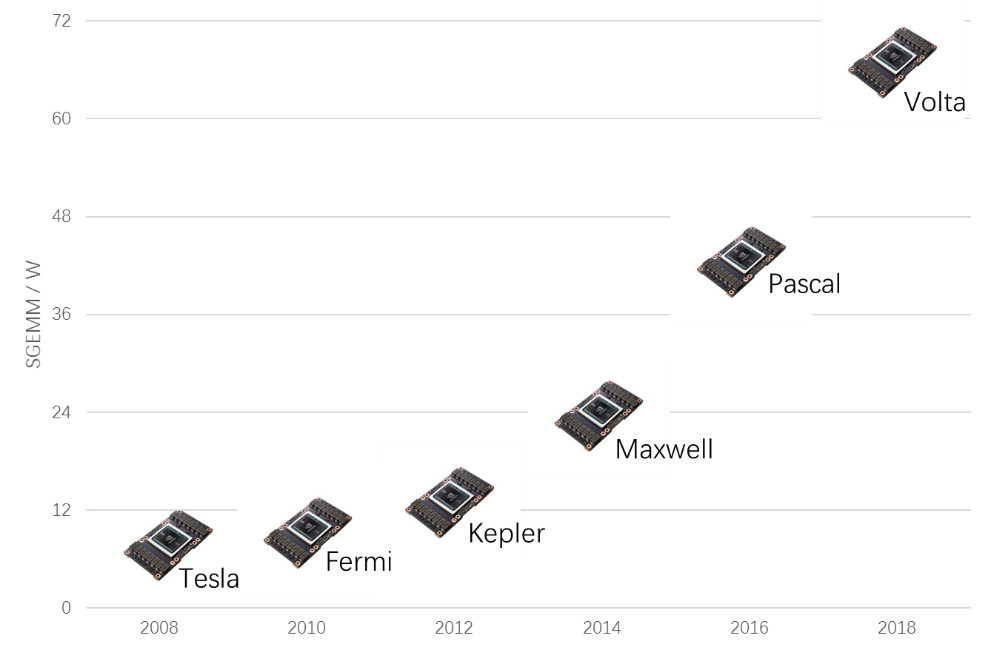
\includegraphics[width=0.40\textwidth]{nvidia_roadmap}
	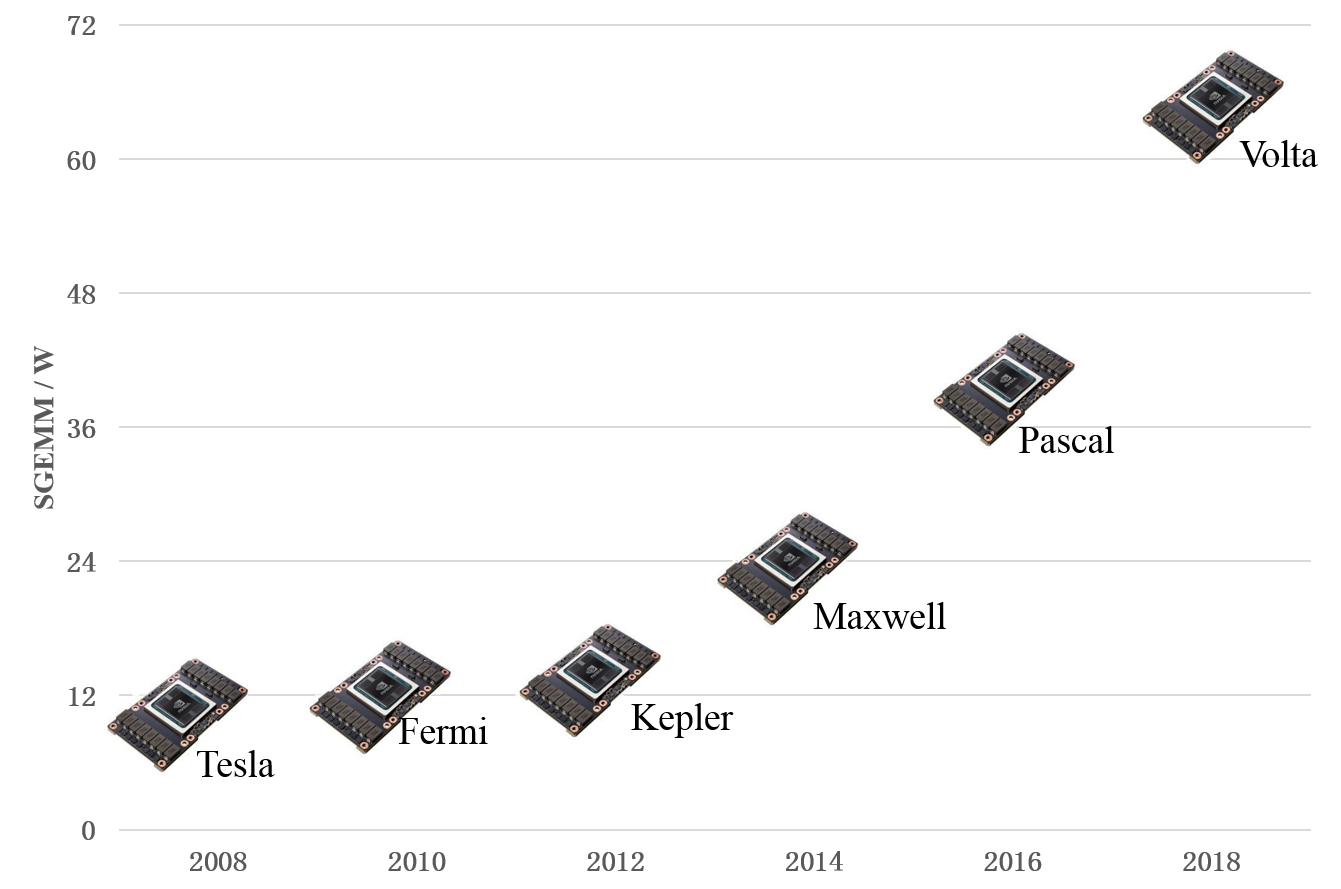
\includegraphics[width=0.60\textwidth]{nvidia_gpu_roadmap}
	\bicaption{NVIDIA GPU架构演进图}{NVIDIA GPU Architecture Evolution}
	\label{fig:nvidia_gpu_roadmap}
\end{figure}

AMD提出的GCN(Graphic Core Next)相较之前提出的VLIW架构是一个分水岭。AMD GPU历经了Polaris,Vega,Navi架构的演进(如图\ref{fig:amd_roadmap})。这几种系列的产品都采用了GCN架构。GCN架构具有灵活的可编程性,较好的编译工具链的支持,可极大发挥出GPU的计算能力。
\begin{figure}[!htbp]
	\centering
	%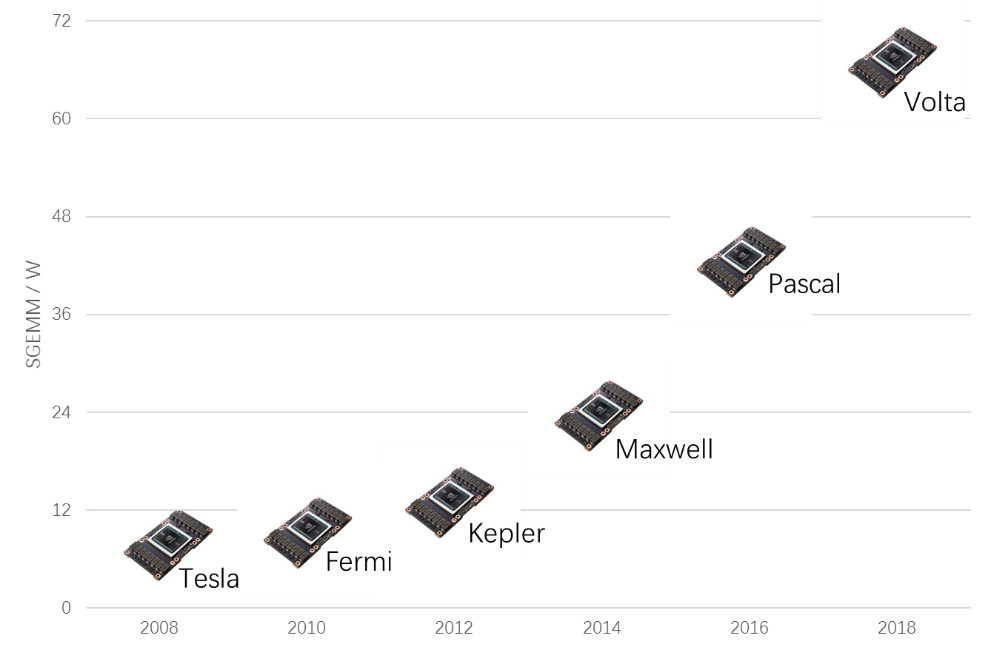
\includegraphics[width=0.40\textwidth]{nvidia_roadmap}
	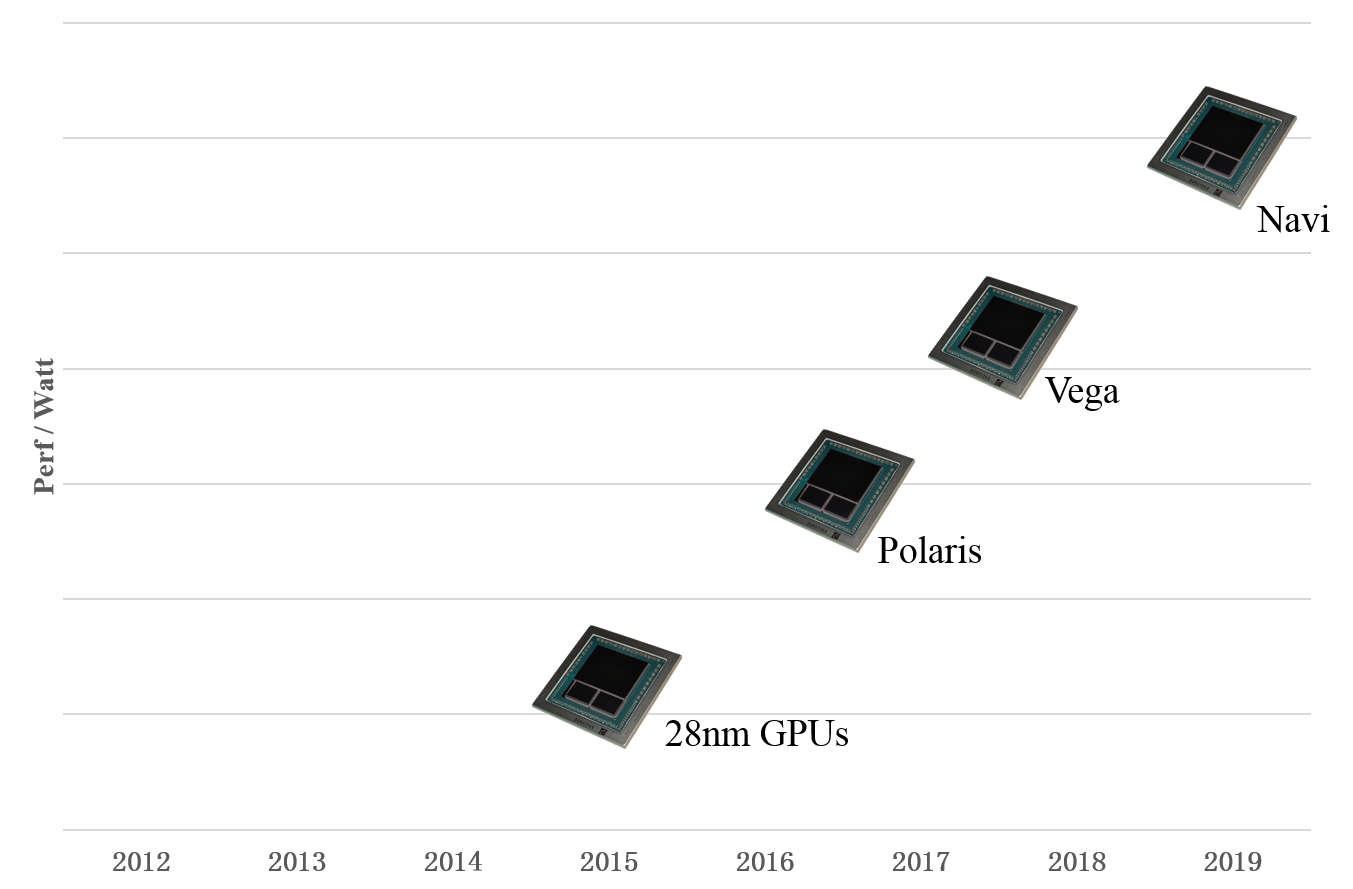
\includegraphics[width=0.60\textwidth]{amd_roadmap}
	\bicaption{AMD GPU架构演进图}{AMD GPU Architecture Evolution}
	\label{fig:amd_roadmap}
\end{figure}

\section{并行计算技术概述}
计算可分为串行计算和并行计算。为了引出并行计算的概念,我们先从串行计算开始介绍。在计算机发展的早期,程序编制人员编写的通常是串行软件。串行软件有这几个特点:(1) 将要处理的问题分解为一系列的指令,(2) 这些指令按照顺序一条一条执行,(3) 所运行的处理器只有一个核心,(4) 在同一时刻只能有一条指令在执行(如图\ref{fig:serialprogram})

\begin{figure}[!htbp]
	\centering
	%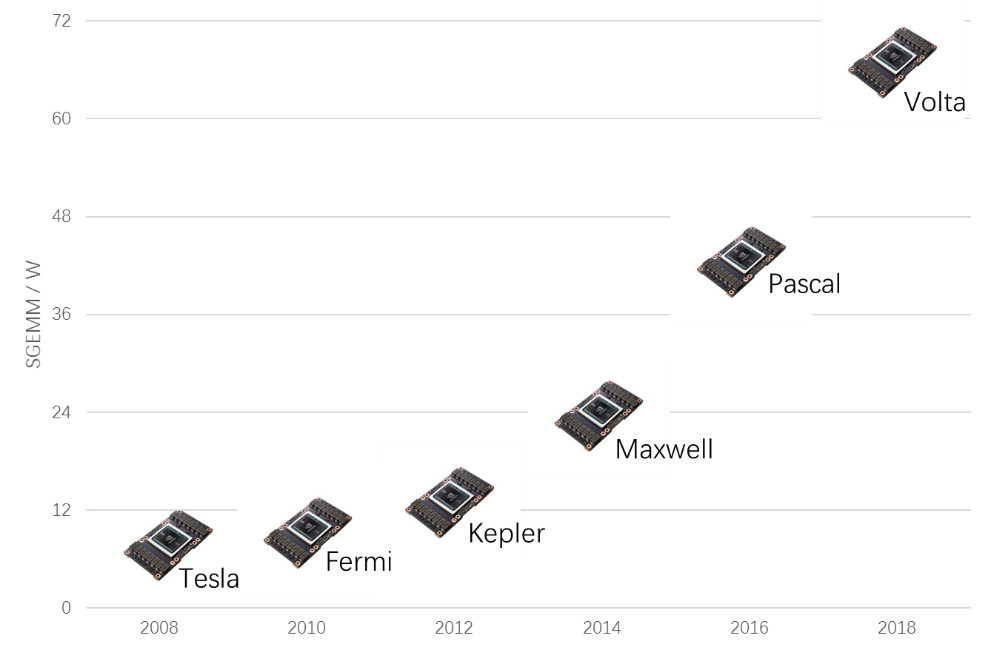
\includegraphics[width=0.40\textwidth]{nvidia_roadmap}
	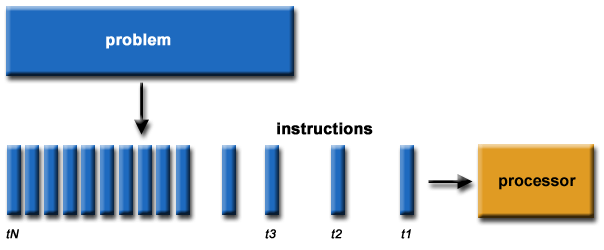
\includegraphics[width=0.60\textwidth]{serialprogram}
	\bicaption{串行程序执行示意图}{Serial program execution diagram}
	\label{fig:serialprogram}
\end{figure}

接下来引入并行计算的概念。从简单意义上来讲,并行计算是同时使用多个计算资源来解决计算问题。并行计算具有如下几个特点:(1) 将一个问题分解成可以同时求解的几个子问题,(2) 每个子问题同时在不同的处理器上计算,(3) 有一个总的控制协调机制(如图\ref{fig:parallelprogram})

\begin{figure}[!htbp]
	\centering
	%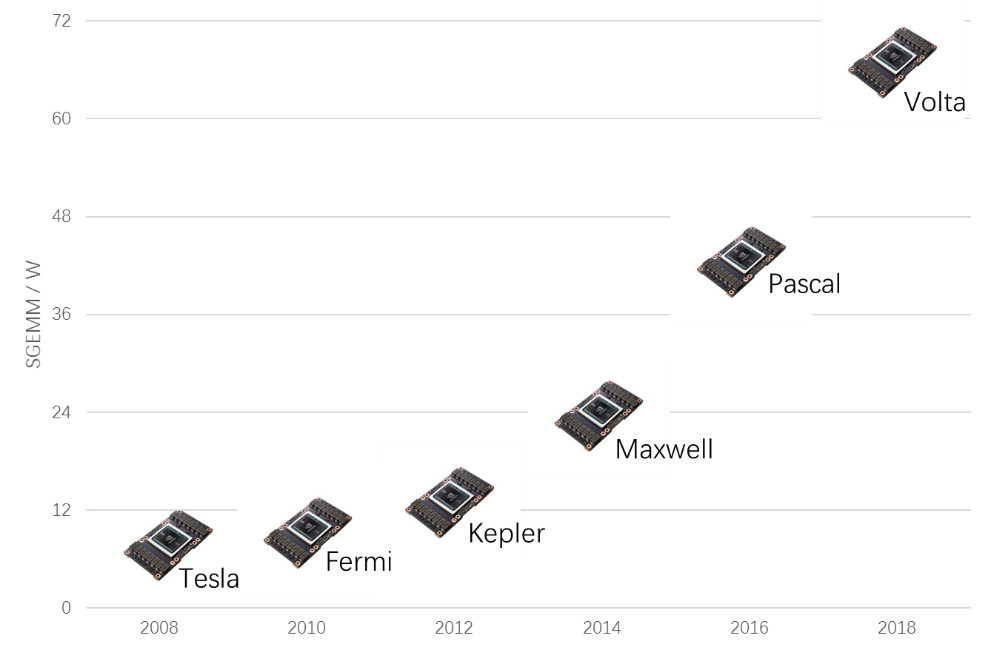
\includegraphics[width=0.40\textwidth]{nvidia_roadmap}
	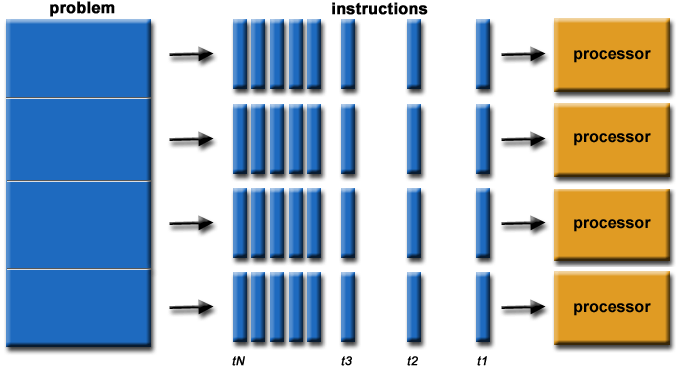
\includegraphics[width=0.60\textwidth]{parallelprogram}
	\bicaption{并行程序执行示意图}{Parallel program execution diagram}
	\label{fig:parallelprogram}
\end{figure}

并行计算的主要目标是通过提高计算资源的利用率来使得应用程序运行的更快。通常情况下,并行计算的基础设施可以是服务器机架上的一个多个处理器或者许多单独的服务器通过网络连接在一起的服务器集群。将计算任务划分成一个个子任务,Server端将每个子任务的计算请求发送到每个处理器(线程),每个处理器(线程)执行自己的子任务,最后Server端合并计算的结果。并行计算可以分为指令集并行,数据并行和任务并行。


\section{研究动机述}
矩阵乘是BLAS(Basic Liner Algebra Subprogram) Level3标准中定义的数学计算,是BLAS库的核心子程序之一。虽然BLAS规范是通用的,但是BLAS库的实现通常都针对特定硬件进行着专门的优化,使得BLAS库具有显著的性能优势。BLAS库在实现上利用特殊的浮点硬件(如向量寄存器,SIMD指令等)来提高计算速度。BLAS库的例子包括:AMD核心数学库(ACML),ATLAS,英特尔数学核心库(MKL)和OpenBLAS。ATLAS是一个可自动调优的,适用于任意硬件架构的可移植库。MKL是英特尔官方提供的针对英特尔处理器进行了专门优化的数据库。OpenBLAS是一个开源库,针对许多主流的体系结构进行了手工优化。LINPACK程序的跑分在很大程度上依赖于BLAS库中DGEMM的子程序的性能。BLAS库被广泛应用于高性能计算领域,近几年兴起的深度学习,其核心计算也依赖于BLAS库的性能。

矩阵乘的计算复杂度为$O(N^3)$,访存复杂度为$O(N^2)$,这种计算密集型的特点非常适合用GPU来加速\citepns{nath2010improved}。然而由于GPU独有的并行结构需要高度调优的kernel来达到性能峰值\citepns{kurzak2012autotuning}。当前GPU架构仍在持续演进,GPU应用的领域越来越广泛,人们对应用程序性能的极致追求推动着GPU程序调优工作的进行\citepns{cui2010auto}。

矩阵乘的效率通常可以展示一个计算机系统实际可达的最高计算性能。通过对矩阵乘性能的调优和性能分析,可以深入理解现代多核处理器体系结构的方方面面。同时,也将提高BLAS库Level3的计算性能,从而提高基于BLAS库的应用的计算速度。

DNN(Deep Neural Network)是深度学习的一个主要方向。由于DNN的强大的表达能力,使得人们可以使用其解决各种领域里的问题。当前的DNN几乎代表了机器学习的主要发展方向。在DNN网络中,有大量的参数,使得做训练和推理的过程变得非常耗时。特别是,全连接和卷积层的矩阵乘(Matrix Multiplication)计算成为了DNN计算的瓶颈。计算机科学家和工程师们花费了很多年来研究如何提高DNN的计算效率。

在GPUs出现之后,DNN开始流行起来。因为相比于CPU,GPUs可以将矩阵乘的计算速度提升几十到几百倍。在此期间,NVIDIA开发出了专门用于DNN训练和推理的数学库cuDNN\citepns{chetlur2014cudnn},由于该库的鲁棒性和高性能,cuDNN已经成为了当前的工业标准。cuDNN中矩阵乘的实现对于各种输入尺寸,在不同的GPUs架构上都可以获得较高的性能。另外,cuDNN作为后端,已经广泛用于各种DNN框架中,例如caffe、pytorch、tensorflow和mxnet。所以,提高矩阵乘的效率,可加速DNN的训练和推理过程。


\section{本文主要贡献}
本文工作是基于AMD GPU平台,实现了面向GPU体系结构的通用矩阵乘优化,以解决当下AMD GPU矩阵乘效率低的问题,并且对AMD GPU矩阵乘进行了性能分析,为优化AMD GPU其他应用程序提供了性能分析方法。论文的主要工作如下:

% (1) 深入理解AMD GPU体系结构,比较了NVIDIA GPU和AMD GPU在架构设计上和程序执行模型上的异同。
%
% (2) 分析了NVIDIA GPU矩阵乘的效率,总结出NVIDIA GPU矩阵乘的优化手法。

% (1) 基于对NVIDIA GPU矩阵乘算法以及优化方法的理解,将该方法结合AMD新一代GPU Fiji和Vega10架构的特点,提出AMD GPU矩阵乘算法以及调优方法。

 (1) 针对新一代AMD GPU体系结构的特点,设计出一套AMD GPU微基准测试程序,并探测出AMD GPU浮点指令的通量和内存带宽。

 (2) 实现了面向AMD GPU体系结构的通用矩阵乘计算,通过对AMD GPU架构的理解,利用指令预取、双缓冲、bank冲突消除、指令重排等调优方法,提高了AMD GPU矩阵乘的效率。

 (3) 通过对矩阵乘主循环中浮点指令和访存指令在不同百分比下指令通量的测试,分析了矩阵乘的性能上界,并将Roofline模型应用到AMD GPU矩阵乘的性能分析中。


\section{本文组织结构}
本文总共分为七章。

第一章概述了课题的研究背景。讲述GPU体系结构的发展历程以及当前主流应用对并行计算的需求,凸显本课题的研究动机和意义,并介绍了研究内容和主要贡献。

第二章介绍了技术背景和相关研究。首先对矩阵乘的几种常用算法进行描述,对每种算法的优缺点和使用场景进行简单概述。然后介绍目前已有的矩阵乘优化加速工作,分析其方法的优点以及存在的问题。

第三章对主流的多核和并行处理器体系结构的原理进行详细介绍,分析多核体系结构对程序性能的影响,为后文讲述矩阵乘算法在AMD GPU平台上的实现进行铺垫。

第四章介绍了GPU体系结构的特点,GPU程序的组织和执行模式。包括了GPU的内存层次结构,GPU的计算单元的组织方式,GPU的硬件计算单元如何与软件线程关联起来,GPU的编程模型,程序的执行模式。其中核心的概念是GPU的SIMD(或SIMT)执行方式。NVIDIA和AMD GPU在设计上都采用这种执行方式。

第五章讲述了矩阵乘GPU实现的算法和具体实现步骤。描述了矩阵乘外积法的执行过程,并分析了外积法相比于內积法的优势。通过三个步骤讲述了外积法矩阵乘计算过程中,数据的搬运和计算的执行过程。为下一章节讲述矩阵乘调优过程做铺垫。

第六章以AMD Fiji和Vega10 GPU为实验平台,进行了AMD GPU矩阵乘算法的设计和调优。进行矩阵乘性能测试,分析AMD GPU矩阵乘性能上界。

第七章对全文进行总结,并提出未来可能的研究方向。




\chapter{背景及相关研究}\label{chap:background}
本章首先概述GPU体系结构的相关知识和研究人员在不同GPU架构上实现的矩阵乘算法,引出AMD GPU矩阵乘相关的背景知识。然后介绍目前国内外对GPU矩阵乘的调优工作。最后一小节介绍本文工作所采用的AMD GPU体系结构的相关知识,以帮助理解本文中使用的矩阵乘调优方法。

\section{GPU架构概述}

GPU(Graphics Processing Units)设计之初是为了做图形渲染。在图像渲染中,大部分工作是在进行顶点和像素的处理,由于顶点和像素处理具有天然的并行性,所以GPU的发展方向就是大量“轻型”线程,可以快速进行任务切换。由于具有大量并行“轻量”线程的特点,以及复杂的硬件动态调度,是的GPU具有很好的延迟容忍特性。

从线程的概念上,GPU的线程由应用程序,驱动,运行时库和硬件调度器进行控制。GPU的线程更为底层,接近硬件。CPU端的线程更为上层,由操作系统控制线程的创建,调度和回收等工作。

从应用场景上,GPU可以分为移动端,桌面端和服务器级GPU。移动端GPU的特点是要做到功耗,同时也要具有较高计算性能。桌面端和服务器级GPU则追求更高计算性能,对功耗则没有非常苛刻的要求。为了实现高访存带宽,GPU的大量引脚被用来连接内存,并且使用GDDR5高带宽访存协议。

在计算单元的设计上,AMD和NVIDIA GPU的计算单元都采用了SIMD(Single Instruction Multiple Data)(或者SIMT Single Instruction Mulitiple Thread)架构。在术语上,AMD称其为SIMD,NVIDIA称其为SIMT或SPMD(Single Program Multiple Data)。AMD GPU由很多CU(Compute Units)组成,NVIDIA GPU由很多SM(Streaming Multi-processors)或SMX组成。对于AMD Redeon Vega10架构,每个CU有4个SIMD部件,每个SIMD的宽度为16。通过向量流水线的方式用4个时钟周期来执行宽度为64的向量操作。对于NVIDIA GTX780,其设计为Kepler架构,每个SMX有12个SIMD,每个SIMD的宽度为16。通过2个时钟周期来执行宽度为32的向量操作。

对于AMD GPU GCN架构,每个CU包含一个标量部件和4个SIMD部件,每个SIMD最多可以有10个向量线程(AMD称为wavefronts)in flight,向量线程的宽度为64。一个SIMD在每个指令发射周期选择一个向量线程来执行。所以,一个CU最多可以运行40个向量线程。NVIDIA GPU在设计上也与之类似。但实际可运行的向量线程数受很多因素限制,这里包括寄存器数量,局部共享内存的大小等。

对于AMD GPU和NVIDIA GPU体系结构,采用了SIMD的编程模型,每个线程是SIMD中的一项。NVIDIA称之为“SIMT(Single Instruction, Multiple Thread)”或者“SPMD(Single Program, Multiple Data)”。对于AMD GPU,一个wavefront有一个程序计数器,指令的分支由专门的寄存器做掩码来标记,控制每个线程的行为。

通过上面的比较,可以看出,AMD GPU和NVIDIA GPU都采用了SIMD结构,不同的是AMD GPU所计算的向量的宽度为64,NVIDIA GPU所计算的向量宽度为32。由此可以窥见SIMD结构代表着现代GPU的主流设计方向。




\section{GPU线程执行模型}
本文旨在基于AMD GPU平台,对矩阵乘算法进行实现和优化。为了实现更高效的矩阵乘,编程人员必须深入分析GPU体系结构的组织方式和GPU程序的编程和执行模型。

GPU程序的逻辑调度和执行单元是block,在术语上,NVIDIA称为thread block或block,AMD称为work-group。一个block中的所有线程共享一个shared memory。在硬件上,一个block执行时位于某一个SMX(CU)中。Block的执行不能跨SMX(CU)。一个block包含一到多个warp(wavefront)。一到多个block组成一个grid(NDRange)。如图\ref{fig:thread_model}展示了AMD GPU线程的组织方式。一个warp有32个线程,wavefront有64个线程,OpenCL中称为work-item。

\begin{figure}[htbp]
	\centering
	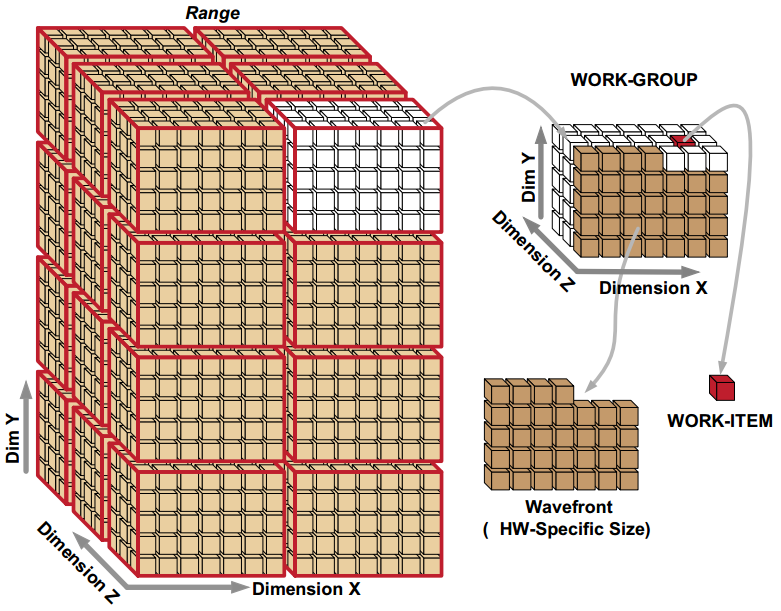
\includegraphics[width=0.50\textwidth]{thread_model}
	\bicaption{work-item,wavefront和NDRange之间的关系}{The relationship between work-item, wavefront and NDRange}
	\label{fig:thread_model}
\end{figure}

在线程执行模式上,NVIDIA GPU以warp为单元调度和执行,一个warp有32个线程,一个warp中的线程协作执行(如图\ref{fig:warp_model})。AMD GPU以wavefront为单元调度,一个wavefront有64个线程。在warp(wavefront)执行过程中,遇到分支时,在时间上来看,是“串行”执行的(如图\ref{fig:if_else},\ref{fig:warp_if_else})。

\begin{figure}[htbp]
	\centering
	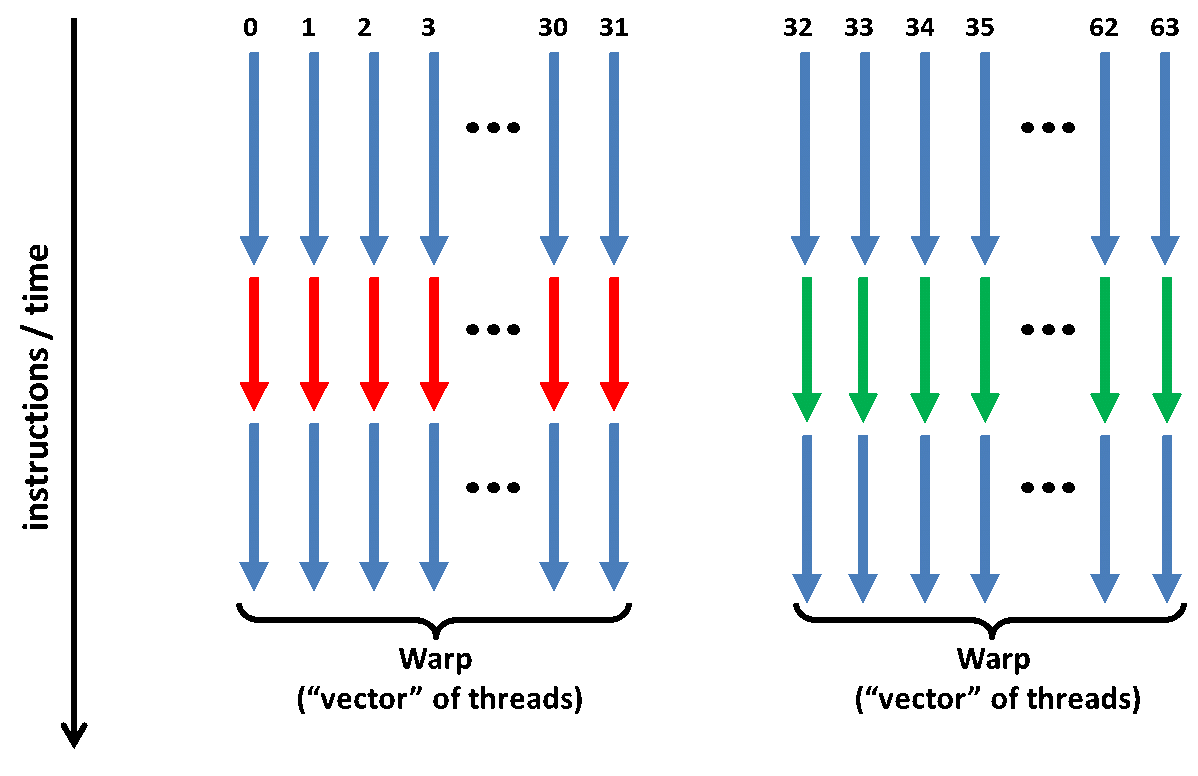
\includegraphics[width=0.50\textwidth]{warp_model}
	\bicaption{NVIDIA warp执行模式}{NVIDIA warp execution model}
	\label{fig:warp_model}
\end{figure}


\begin{figure}[htbp]
	\centering
	%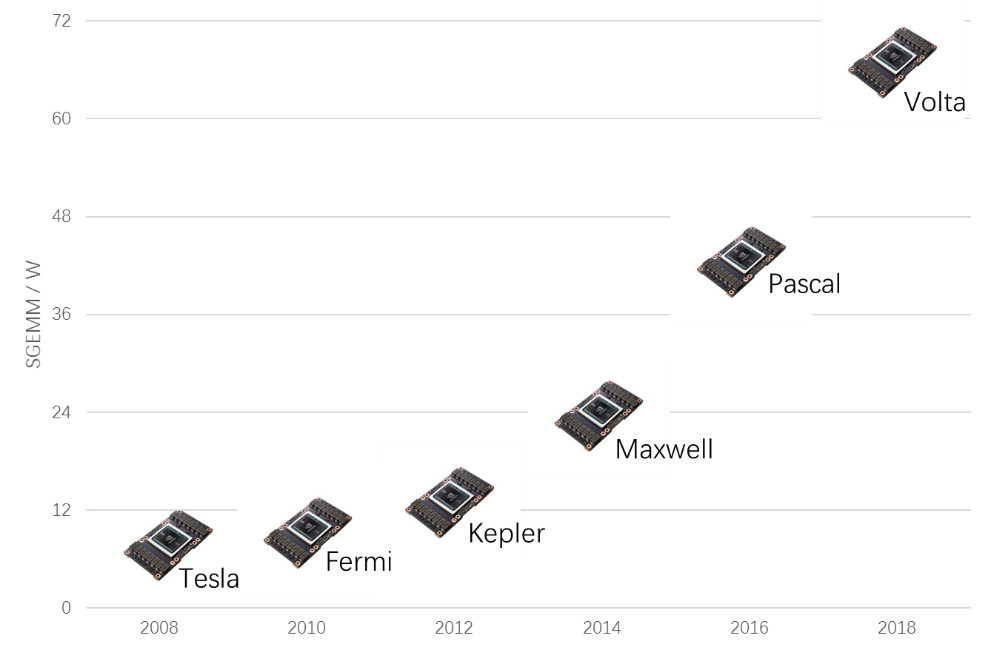
\includegraphics[width=0.40\textwidth]{nvidia_roadmap}
	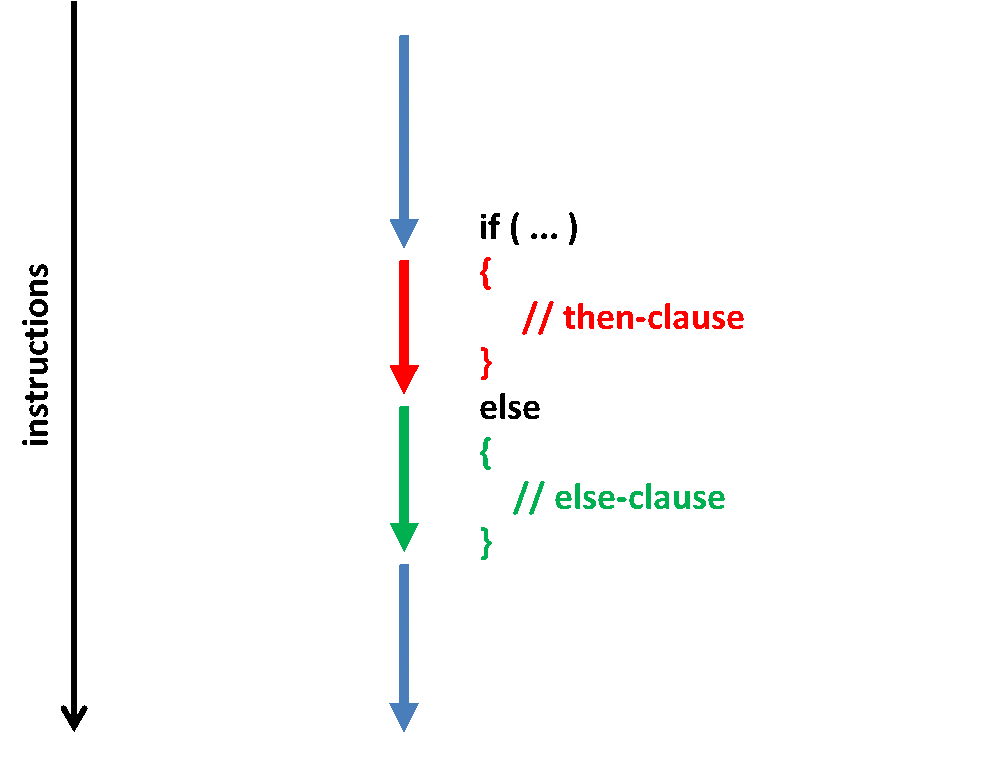
\includegraphics[width=0.50\textwidth]{if_else}
	\bicaption{if-else分支控制流}{If-else branch control flow}
	\label{fig:if_else}
\end{figure}

\begin{figure}[htbp]
	\centering
	%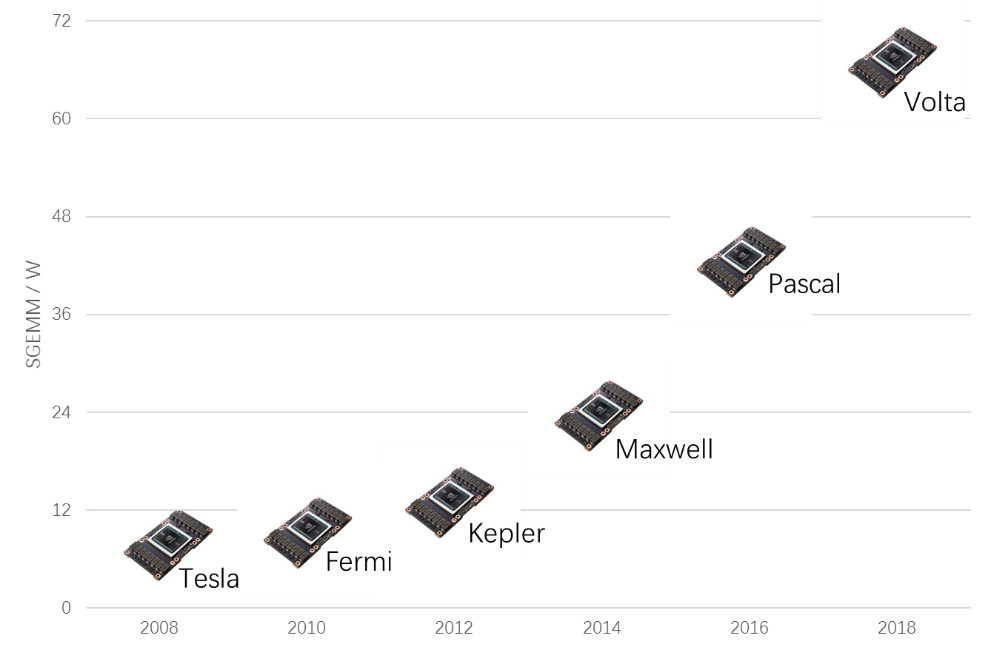
\includegraphics[width=0.40\textwidth]{nvidia_roadmap}
	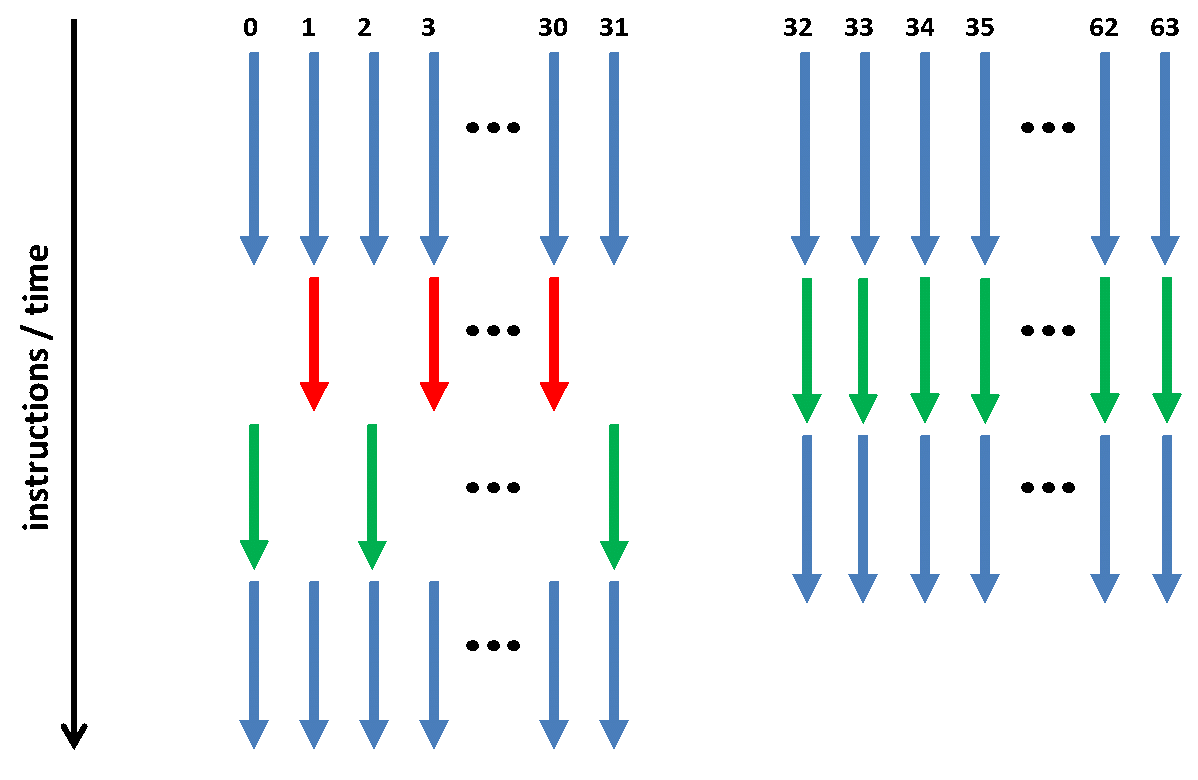
\includegraphics[width=0.50\textwidth]{warp_if_else}
	\bicaption{warp(wavefront)执行if-else分支流图}{Warp(wavefront) executes if-else branch flow graph}
	\label{fig:warp_if_else}
\end{figure}

由此,可以看出在设计GPU程序时,尽量减少指令分支。因为分支将导致程序“串行”执行,极大降低了执行速度。在接下来的章节里,将讨论如何设计GPU程序,以使线程的执行步调尽可能一致。从而提高执行速度。

\section{现有矩阵乘调优工作}
在本小节中,首先给出矩阵乘的标准数学表达,然后介绍现有矩阵乘在多核处理器上的研究工作。

\subsection{矩阵乘数学定义}
矩阵乘(GEMM General Matrix Multiply)数学表达为

\begin{equation}
	C:= \alpha op(A)*op(B) + \beta C
\end{equation}

其中A,B,C为矩阵,$\alpha$,$\beta$ 为标量。op 表示矩阵是否转置,即op(X) = X 或 op(X) = $\mathbf{X}^\mathrm{T}$。

\subsection{矩阵乘在多核处理器上的研究介绍}
目前国内外对矩阵乘的调优工作主要集中在NVIDIA GPU和各种主流CPU。NVIDIA在2010年设计出了第一款Fermi架构GPU。Fermi架构也影响着此后NVIDIA GPU架构的演变。Volkov\citepns{volkov2008benchmarking}通过benchmark的方法做了8系列,9系列和200系列NVIDIA GPU矩阵乘调优工作。

Junjie Lai\citepns{lai2013performance}在Fermi和Kepler架构上通过SGEMM(Single-precision General Matrix Multiply)算法性能分析和汇编级的微基准程序测试,提出了一套分析GPUs应用程序性能上界的方法。Junjie Lai通过分析发现,Fermi(Kepler)指令集自身的特点和调度器有限的发射通量是限制SGEMM通向理论峰值的两个主要因素。Lai评估了SGEMM的性能上界在GTX580 Fermi GPU为理论峰值的82.5\%,在GTX680 Kepler GPU为理论峰值的57.6\%。

Scott实现了第一个NVIDIA Maxwell架构开源汇编器MaxAs\citepns{grayassembler}。基于该汇编器,手写了非常高效的矩阵乘和卷积kernel。其实现的SGEMM在Maxwell架构上达到理论吞吐量的98\%,比NVIDIA官方库cuBLAS\citepns{nvidia2008cublas}汇编矩阵乘要快4.8\%。并写了一个微基准测试框架,为指令调度做铺垫。在开始这项工作之前,Scott仔细研究了cuBLAS在Kepler和Maxwell架构上的矩阵乘实现。Maxas SGEMM是Junjie Lai工作的一个扩展,针对Maxwell架构做了汇编级的调优。相比于Lai的工作,Scott破解的了Maxwell架构汇编控制码的含义,为实现更细粒度指令调度提供了可能。Scott在64线程的矩阵乘实现中,计算得出的矩阵乘性能上界为98.5\%(表\ref{tab:maxwellFFMA})。
\begin{table}[htbp]
	\bicaption{矩阵乘主循环指令构成}{GEMM main loop instructions}
	\label{tab:maxwellFFMA}
	\begin{center}
		\begin{tabular}{ | l | p{3cm} |}
			\hline
			Operation & Count \\ \hline
			FFMA & 512  \\ \hline
			LDS.128 & 32 dual issue \\ \hline
			STS.128 & 4 dual issue \\ \hline
			TLD.128 & 4 dual issue \\ \hline
			IADD & 4 \\ \hline
			XOR & 3 \\ \hline
			SETP & 1 \\ \hline
			BAR & 1 dual issue \\ \hline
			BRA & 1 daul issue \\
			\hline
		\end{tabular}
	\end{center}	
\end{table}

FFMA通量为512/(512+4+3+1)=512/520 = 98.5\%。其他指令是双发射的,不计入计算中。其中,指令的双发射由控制码进行控制。

Zhang\citepns{zhang2017understanding}实现了Kepler架构第一个开源汇编器KeplerAs\citepns{xiuxiaassembler},填补了Kepler GPU无可用汇编器的现状。Zhang在Scott和Lai工作的基础上,破解了Kepler K20 GPU架构的控制码,探测出Kepler GPU寄存器bank分布。利用Kepler架构独有的FFMA双发射,在NVIDIA kepler K20m上实现了更快的SGEMM,性能为3.1Tflop/s,达到88\%的计算效率,高出cuBLAS7.0 15\%。优化的卷积高出cuDNN4.0 39\%$\sim$62\%。

德州大学奥斯汀分校的Goto等人在2005年编写了基本线性代数库GotoBLAS。在BLAS Level-3中针对GEMM(General Matrix Multiply)做了优化\citepns{goto2008anatomy}。GotoBLAS作者在2010年去了微软工作,之后GotoBLAS停止了更新和维护。在2011年中科院软件所张先轶等人基于GotoBLAS发起了OpenBLAS\citepns{xianyi2012openblas}项目,OpenBLAS在各种主流CPU上都获得了比较高的性能。以OpenBLAS库为核心技术的彭峰科技取得了商业上的成功。但OpenBLAS主要针对CPU端做了十分细致的优化,而在GPU上做的优化工作则比较少。

实现GPU (Graphic Processing Units)上的快速通用矩阵乘一直以来都是自动调优工具和kernel编写人员所追求的目标。在本篇文章中,我们尝试提供一种GPUs上算法性能上界的方法,并做出汇编级的基准测试。Meng等人\citepns{meng2011grophecy}提出了GPU性能预测框架,该框架基于标注代码框架。Hong和Kim提出了MWP-CWP\citepns{hong2009analytical}模型来预测CUDA应用程序性能,该模型基于NVIDIA PTX。Sim\citepns{sim2012performance}等人在2012年将MWP-CWP模型进行了扩展,使用汇编编写kernel预测程序性能。Zhang和Owen\citepns{zhang2011quantitative}基于汇编程序提出了GPU定量分析模型。由于关于GPU微架构的资料非常少,我们无法针对新一代GPU架构做出精确的GPU模拟器。但我们通过上面这些分析方法可以十分近似的预测GPU程序的性能。Roofline\citepns{williams2009roofline}模型是应用最广的用来评估优化效果的模型,本文将采用该模型对SGEMM做性能分析。

\section{本章小结}
本章首先概述GPU体系结构的相关知识和研究人员在不同GPU架构上实现的矩阵乘算法,引出AMD GPU矩阵乘相关的背景知识。然后介绍矩阵乘的数学定义,目前国内外GPU矩阵乘的调优工作。最后一小节介绍本文工作所采用的AMD GPU体系结构的相关知识,以帮助理解本文中使用的矩阵乘调优方法。





\chapter{并行处理器架构分析}\label{chap:parallelArch}
在计算机发展的早期,CPU的主频呈上升趋势。程序的性能随着处理器主频的提升而得到相应提升。但2007年之后,由于功耗和散热的限制,处理器的主频无法继续得以提升。单核性能无法再得以提升。处理器开始往多核方向发展。如何提升程序在多核处理器性能成为了软件编程人员所面临的问题。在实际应用程序中,大多数情况下,随着CPU核数的增加,程序性能并不是线性提升,多核的利用率非常低。编程人员开始思考如何程序在多核处理器上的性能,从而充分发挥多核处理器的计算能力,提高程序的执行速度。

\section{并行计算介绍}
在2007年以前,CPU的主频呈上升趋势。我们程序的性能随着处理器主频的提升而得到相应提升(如图\ref{fig:cpu_trend})。但在此之后,由于功耗和散热的限制,处理器的主频无法继续得以提升。这个主要原因是,处理器的功耗和频率是非线性关系。
\begin{figure}[htbp]
	\centering
	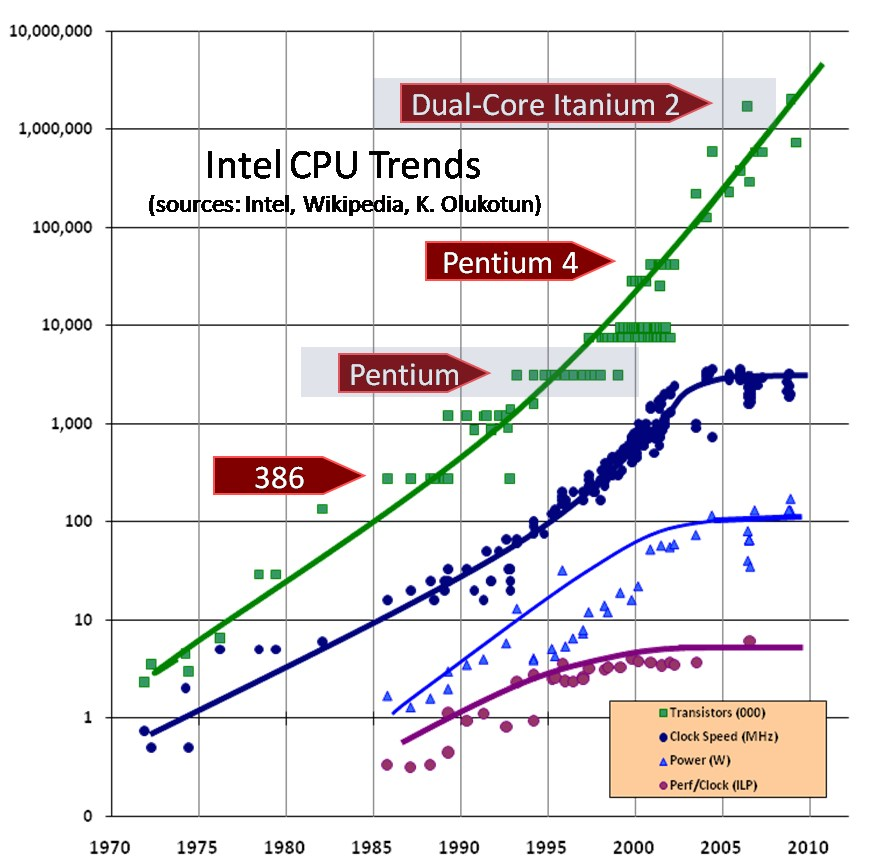
\includegraphics[width=0.50\textwidth]{cpu_trend}
	\bicaption{Intel CPU发展趋势}{Intel CPU trends}
	\label{fig:cpu_trend}
\end{figure}
为了具体说明主频和功耗之间的关系,下面给出CMOS功耗的计算公式。CMOS的处理器内部的基本半导体元件。
CMOS(互补金属氧化物半导体)的功耗公式:
\begin{equation}
	\label{eq:power}
	P=ACV^{2}F+VI_{leak}
\end{equation}

其中,P表示CMOS的功耗,A表示活动因子,C表示电容,V表示电压,F表示开关频率,$I_{leak}$表示漏电流。公式的前半部分表示动态功耗,后半部分表示静态功耗。从上面的公式看起来功耗与频率成线性关系。但实际上,要提升频率,就要增加电压,同时增加了动态功耗和静态功耗。所以,频率的一点点提升,都会带来功耗的巨大增加。

从另外一个方面来考虑,随着处理器主频的提升,处理器的计算速度和访存的速度差距进一步拉大。此时,我们需要考虑增大访存带宽,或者增大L1、L2 Cache来减小这种鸿沟。为了获得更强的计算性能,处理器开始朝着多核、众核方向发展。

从编程人员的角度,我们习惯于编写串行的程序。一个任务做完后,开始做下一个任务,这样依次做下去。随着多核、众核处理器的发展,并行程序的编制需求越来越多。但并行程序难以编写和调试的特点很大程度上影响了并行软件的开发速度。为了开发出高效的并行程序,一般要求编程人员不仅有并行程序的编写和调试经验,也要深入理解处理器架构的细节。

GPU在设计上是一种并行处理器,数据并行计算任务可充分发挥出GPU的计算能力。矩阵乘是一种典型的并行计算任务,研究GPU矩阵乘的实现和调优不仅可以了解GPU微架构,同时也能极大加速基于矩阵乘的上层应用。



\section{并行处理器架构}
早期的处理器设计者和应用软件开发人员都认为像SIMD这种结构的处理器只是在特定应用场景下可以获得极大的性能提升,但在其他场景下获得的性能提升极为有限。所以,在并行处理器(如GPU)出现以前,多核处理器一直朝着提高单线程的计算能力的方向发展。设计高性能处理器的一个总目标是,提高每个时钟周期可以执行的计算操作的数目。

\subsection{超标量和VLIW}
在CPU设计的很长一段时间,已经出现了超标量、乱序执行。在设计上,处理器自动分析和保存指令流内部依赖关系,生成一张DAG图(有向无环图)。彼此没有依赖的指令可以同时发射,存在依赖关系的指令按序发射。这样可以在一个时钟周期发射多条指令。最后对执行完的指令进行重排,然后顺序提交。通过这种方式可以提高处理器的整体利用效率。现代的CPU大多是超标量处理器,也有部分GPU具有超标量处理的能力。

VLIW(Very Long Instruction Word)处理器与超标量处理器的区别在于,超标量处理器的多发射是由硬件调度的,而VLIW处理器的多发射是由编译器在做的。编译器将没有依赖的指令打包成一个VLIW,形成VLIW的指令流。交由硬件来执行。每个时钟周期发射一个VLIW指令。从控制逻辑上,VLIW处理器比超标量处理器简单,不需要从硬件层面上动态分析指令依赖图。

VLIW处理器的效率依赖于编译器和具体的指令流。如果实际的指令流可以很好的吻合VLIW的硬件结构,并且编译器也可以很好地将指令流打包成一个个VLIW,那么就可以充分发挥出VLIW处理器的性能。否则,就无法有效利用VLIW处理器。


\subsection{GPU的SIMD结构}
SIMD(Single Instruction Multiple Data)即单指令多数据流,SIMD结构的处理器直接在一条指令中对多个数据做相同的并行操作。所以SIMD结构的处理器是一种数据并行处理器。SIMD指令按序执行,一次执行一个向量指令。向量的长度为SIMD处理器的宽度。

尽管SIMD执行是顺序发射的,但我们也可以做到像超标量处理器或者VLIW处理器那样的多发射。

SIMD可以在一个时钟周期对多个数据做相同的操作,很大程度提高了每个时钟周期的计算操作。SIMD结构的处理器也有它的缺点,我们前面给出的示例都是恰好可以组装成向量的指令,但在工业场景下,很多代码并不是可数据并行的,所以也很难将这些代码编译成向量指令来发射。在其他情况下,让编译器对串行代码编译成向量指令也十分困难。如果我们不能对指令进行向量化,那么就不能充分利用处理器的SIMD部件,造成计算资源的浪费。

向量处理器最先出现在超算领域。但SIMD技术已经广泛应用在各种处理器中。例如x86 CPU中的SSE(Streaming SIMD Extensions)和AVX(Advanced Vector eXtensions)指令,Power处理器的AltiVec扩展,和ARM的NEON指令。

GPU体系结构从历史上的演变中就包含了SIMD部件,来支持像素的向量化操作。很多现代GPU的设计也都采用SIMD结构。事实上,我们可以称这种处理器为向量处理器,因为在很多情况下,这种向量是一种逻辑的概念。例如AMD的GCN架构处理器,其向量部件的逻辑宽度为64,在实际实现上,是通过宽度为16的SIMD部件,经过4个时钟周期发射一个宽度为64的向量操作。

\subsection{GPU时分多线程技术}
在指令并行和数据并行之外,的第三种并行方式是多线程并行。即并发的执行多个独立的指令流。在大型并行计算机中大量采用了多线程并行技术,同时多线程并行技术在单核CPU上也是十分有用的。我们之前讨论过,无论在硬件层面还是编译器层面,从指令流中提取无依赖的指令进行并行都是十分困难的,甚至在有些情况下是不可能的任务。然而,从两个独立的线程中提取可并行的指令就变得非常容易,因为它们本身就是无依赖的。实现硬件多线程的困难是,我们需要设计额外的部件,来保存多个线程的寄存器,cache等状态信息。

硬件多线程有两种,一种是同时多线程(SMT),另一种是时分多线程。SMT技术是,将多个线程在处理器上交替地占用计算资源,每种线程看上去都是超标量的执行方式。可以认为是一种多线程超标量的执行方式。

SMT设计的目标是尽可能地将可用计算资源都利用起来。SMT方法带来的代价是需要更多资源来保存每个线程的状态,分析指令间的依赖和调度逻辑也变得更加复杂,因为现在要保存和维护多个线程的状态。
另一种多线程技术是时分多线程。这种技术是,将线程的执行按时间片来划分。用轮询的方式进行调度。

时分多线程的好处是,指令的调度逻辑相对简单、可以通过调度更多的线程来掩盖流水线延迟、单个线程由于cache不命中,分支跳转等带来的停顿可以通过调度更多的线程来掩盖流水线延迟。

当问题扩展到更复杂的情形时,时分多线程就变得非常有用。现代的计算机都可以运行非常多的线程。当一个线程在执行过程中,由于某种原因阻塞了,那么该线程就从就绪队列移到阻塞队列。调度器再从就绪队列的队首取出一个线程执行。一旦阻塞的线程所等待的资源已经获得,该线程就可以从阻塞队列取出,放回到就绪队列中。这种方式就已经非常类似现代操作系统调度线程的方式了。时分多线程的执行方式,尽管单个线程的执行时间会比乱序执行慢很多,但对于整个机器而言,可以保持较高的吞吐量。并且对计算机资源的利用率较为稳定,不需要过分复杂的控制逻辑。考虑线程数不断增加时,处理器需要调度非常多的线程,让处理器充分“繁忙”起来,我们称这种为高通量计算。因为首要考虑的是提高整个处理器的吞吐量。

这两种硬件多线程技术都十分常见。在Tera公司设计的超级计算机MTA(Multi-Threading Architecture)中,就采用了经典的时分多线程技术。但MTA的设计遇到了工艺制造上的困难,随后,Cray设计了MTA-2超级计算机,在设计上,每个CPU拥有128个寄存器,可以实现多线程之间的快速切换,并且在切换时,可以跳过阻塞的线程。Cray公司采用AMD皓龙(Opteron)系列多线程处理器设计了XMT(Explicit Multi-Threading)超级计算机。Sun公司研发的代号为Niagara系列处理器采用了多核,多线程技术,每个核心能同时执行8个线程,用以在数据中心这样的负载中降低功耗和提高吞吐量。Sun的Niagara并不是第一个采用多核,也不是第一个采用多线程技术的芯片,但它比来自于Cray、AMD等公司的芯片更同时注重这两种技术。Intel的Pentium 4、Nehalem以及后续处理器的设计,实现了一种形式的SMT技术,称为超线程(hyperthreading)。现代GPU的设计采用时分多线程技术,可以同时运行大量的线程。实际可运行的最大线程数受到GPU资源的限制(包括寄存器,片上内存等)。对于AMD当前的GPUs而言,每个核心通常可以运行8-16个线程,来掩盖线程停顿和指令延迟。

\subsection{GPU多核结构}
我们至少从概念上认为,提高每个时钟周期执行的任务数最直观的一种方法是在同一个芯片上将单个CPU核简单地“拷贝”多次,做成多核芯片。考虑最简单的情况,每个CPU核的运行都相当独立,通过内存系统来共享数据,通常是通过Cache一致性协议来实现。多核处理器可以看成是经典多套接字服务器对称多处理系统的缩小版。多套接字服务器对称多处理系统是计算机科学家和工程师们在过去十多年追求计算机极致性能所采用的技术体系。

然而,多核系统有不同的表现形式。如何定义一个“核心”,也开始变得困难起来。例如,现在的主流的高端CPU通常包含各种各样的功能区块,这个功能块是独立于计算核心的,如内存控制器,barring接口逻辑等。但我们通常不把这些不讲称为“核心”。然而,这些功能部件和核心之间的界限也可能变模糊。例如,AMD的高功率CPU Steamroller,在两个整数计算核心之间共享一个浮点功能部件(\ref{fig:amd_cpu_core})。
\begin{figure}[htbp]
	\centering
	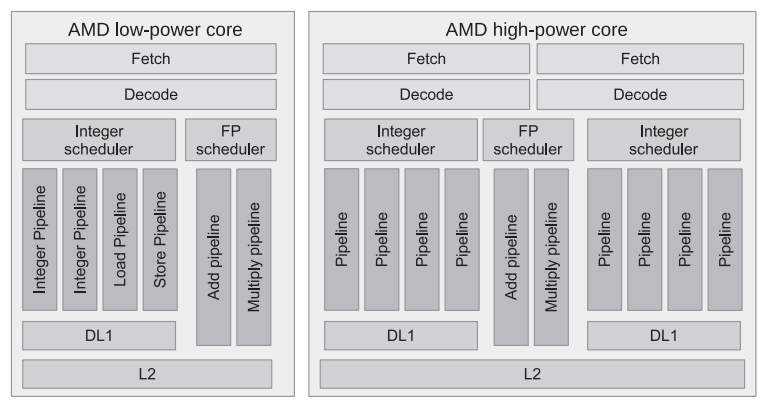
\includegraphics[width=0.50\textwidth]{amd_cpu_core}
	\bicaption{AMD Puma和steamroller架构}{AMD Puma and streamroller architecture}
	\label{fig:amd_cpu_core}
\end{figure}

但AMD低功率CPU Puma则是传统的一个整数计算核心和一个浮点计算核心。单线程在steamroller上执行时,还是按照传统的方式在一个核心执行。但在硬件调度上,两个核心会交替使用浮点计算部件。这种设计的初衷是尽可能提高浮点部件的利用率。

NVIDIA的kepler架构GPU的设计就和Steamroller设计有异曲同工之妙。NVIDIA kepler GPU的SM(Streaming Multi-proccessor)在两个CUDA核心之间共享一个FFMA部件。可以FFMA双发射。

与CPU类似,GPU对“核心”也有不同的定义。现代GPU一般有几十个“核心”。不同架构的高端GPU,其“核心”由32到64不等。许多GPU的设计,如AMD GCN GPUs和NVIDIA的Fermi、Kepler GPUs,都在很大程度上参照CPU的设计风格。例如,AMD Radeon HD6970 GPU,拥有24个SIMD核心。和传统CPU相比,每个SIMD相当于一组ALU,可以做整数和浮点操作,通过wave调度器进行指令的调度,解码和分发(\ref{fig:amd_gpu_core})。
\begin{figure}[htbp]
	\centering
	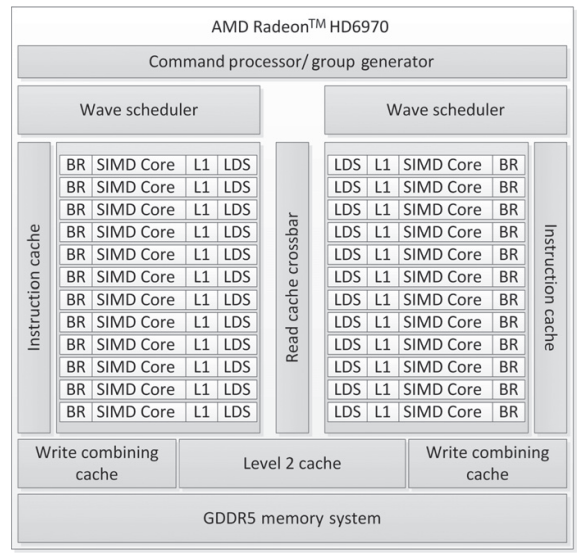
\includegraphics[width=0.50\textwidth]{amd_gpu_core}
	\bicaption{AMD HD6970架构}{AMD HD6970 architecture}
	\label{fig:amd_gpu_core}
\end{figure}

在嵌入式系统中,大多数情况是异构的。既有CPU,也有FPGA、DSP、GPU等加速部件。嵌入式系统的一般特点是,定制化,计算资源受限。追求低成本,低功耗,可长期稳定工作。为了实现低功耗,嵌入式系统开发人员通常会将各种组件放到一块芯片上,做成片上系统(SoC System on Chip)。嵌入式系统在人们的生活中广泛存在。例如,人们使用的手机,智能手环等设备,我们都称之为嵌入式设备。如高通骁龙SoC和德州仪器的OMAP处理器都是典型的嵌入式系统。这种系统一般包含一个ARM处理器,一个移动端GPU,内存控制器和各种无线,多媒体处理组件。现在随着深度学习应用越来越广泛,在移动端做高性能计算的需求也越来越多。其中矩阵乘是深度学习数学库的核心计算。如何在移动端做高效的矩阵乘也成为了一个新的挑战。

对于传统的桌面及服务器端处理器,AMD和Intel各自研发了CPU-GPU的SoC芯片,AMD称之为APU。这种设计的初衷是追求低功耗,低价格和高性能。

\subsection{Cache层次结构和内存系统}
在早期的计算机中,一开始并没有加入Cache。对于早期的超级计算机而言,CPU主频并不高,内存的带宽和延迟和CPU的主频相匹配。当CPU处理数据时,总可以取到它想要的数据而不需要等待很长时间。随着时间的推移,CPU的处理速度和内存的读写速度差异逐步扩大。对于当前的计算机系统,CPU从内存读取数据通常需要几百到几千个时钟周期。对于当前的CPU,其乱序执行的方式使得延迟的隐藏变得非常复杂。

通常,数据的访存模式并不是毫无规律的,而是呈现一定的局部性。这里包含两个方面:

时间局部性:时间局部性描述的是,当前访问的数据在一个很近的将来会再次被访问到。

空间局部性:空间局部性描述的是,在一个小的时间窗口中,会多次访问一段临近的内存地址。

根据这两种局部性,我们可以得出这样一个结论:如果我们在读/写时,可以将一块临近的内存数据“暂存”起来,那么当我们再次读/写时,数据就可以重用。为了利用局部性,CPU的设计者们设计出十分复杂的多级缓存系统,来提升CPU的性能。多级缓存在出现,填补了CPU和内存在速度上的鸿沟。

Cache设计的目的就是减小访存延迟。为了实现这一目标,CPU设计者设计复杂的缓存系统来尽可能将数据“搬到”靠近CPU的算术逻辑单元。因为越靠近算术逻辑单元,CPU读/写数据所需时钟周期数就会越少。另外,从寄存器读/写数据也比从全局内存读/写数据的功耗要低。

对于,面向通量计算的处理器,其对访存的延迟容忍度更高。因为有大量的线程会同时在通量处理器上运行,可以通过线程调度来掩盖从数据请求到结果返回这段延迟时间。现代的GPU可以看成是一种面向通量计算的处理器。对于基于SIMD的编程模型,我们的设计目标是尽可能实现合并访存,来提高单次内存访问的效率。

在现代GPU的设计上,包括了一个可显式编程控制的片上内存空间,其速度和Cache接近。在编写程序时,通过小心合理地使用片上内存,可以使我们的程序获得非常高的性能。同时也比编写其他程序更为复杂。



\section{现有并行处理器和专用加速器介绍}
在工业界,我们并没有看到非常多的处理器类别,来让我们将其完美划分到上面提到的某种类型的处理器种类中。其中的一个主要原因是,现实的应用场景纷繁复杂,每种应用的工作负载都不尽相同。在实际设计处理器时,会尽可能考虑处理器的通用性,以使其可以工作在尽可能多的应用场景中。但这种情况也在近几年慢慢发生变化。随着云计算、深度学习等应用越来越广泛,使得通用处理器已经越来越难以有效地处理这样的工作负载。我们开始转向专用芯片来寻求新的解决方案,ASIC芯片应运产生。例如,谷歌针对自己的Tensorflow框架和数据中心而设计的TPU(Tensor Processing Units)芯片,用以替代CPU和价格高昂NVIDIA GPU。微软针对自己的数据中心设计FPGA芯片。寒武纪针对深度学习应用设计神经网络处理器。

事实上,计算机体系结构有着非常大的设计余地,在每个方向上都有值得深入挖掘的特性。在设计上,ALU,调度器,控制器,Cache,内存的设计在很多方面并不是非此即彼,而是有着很多的权衡。

GPU体系结构的设计有很多权衡。GPU最初开始是为了做图形渲染。做顶点和像素的处理具有天然的并行性。所以,GPU的发展方向就是大量“轻”线程,可快速做任务切换。由于大量并行轻量线程的特点,以及复杂的硬件动态调度,使得GPU具有很好的延迟容忍特性。GPU的线程由硬件进行控制,而不是像CPU那样由操作系统控制。

移动端GPU与桌面端和服务器级GPU相比,移动端GPU一方面要追求较高计算性能,另一方面要做到低功耗。桌面端和服务器级GPU则更加追求高性能,对功耗则没有那么苛刻的要求。为了实现高访存带宽,GPU的大量引脚被用来连接内存,并且使用GDDR5这样的高带宽访存协议。

AMD GPU和NVIDIA GPU的计算单元的设计都采用SIMD架构。在AMD Radeon Vega10架构上,每个CU有4个SIMD,每个SIMD的宽度为16。通过向量流水线的方式用4个时钟周期来执行宽度为64的向量操作。在NVIDIA GeForce GTX780上,其设计上为Kepler架构,每个SMX(Streaming Multiprocessor)由12个SIMD,每个SIMD的宽度为16。通过2个时钟周期来执行宽度为32的向量操作。通过这种比较,我们可以看出,AMD GPU和NVIDIA GPU都采用了SIMD架构,不同的是AMD GPU所计算的向量宽度为64,NVIDIA GPU所计算的向量宽度为32。也可以由此窥见SIMD结构代表着现代GPU的主流设计方向。

对于AMD GPU GCN架构,每个CU包含一个标量部件和4个SIMD部件,每个SIMD最多可以有10个向量线程(AMD称为wavefronts)in flight,向量线程的宽度为64。一个SIMD在每个指令发射周期选择一个向量线程来执行。所以,一个CU最多可以运行40个向量线程。NVIDIA GPU在设计上也与之类似。但实际可运行的向量线程数受很多因素限制,这里包括寄存器数量,局部共享内存的大小等。
对于AMD GPU和NVIDIA GPU体系结构,采用SIMD的编程模型,每个线程是SIMD中的一项。英伟达称之为“SIMT(Single Instruction, Multiple Thread)”或者“SPMD(Single Program, Multiple Data)”。对于AMD GPU,一个wavefront有一个程序计数器,指令的分支由专门的寄存器做掩码来标记。

GPU上的指令级并行。对于AMD GPU每个时钟周期可发射多条向量指令,每个向量指令将被分发到不同的向量单元。AMD GPU的指令可以超标量执行,在同一个CU上,可以同时执行访存指令,计算指令和其他占用不同部件的操作。这样可以提高GPU执行指令的通量。AMD Radeon R9 290X有44个CUs,每个CU包含4个向量单元,共176个向量单元。NVIDIA GeForce GTX 780有12个SMX,每个SMX有12个向量单元,共144个向量单元。这两种GPU都有高速片上内存,在OpenCL的术语中,称之为局部内存。以一个线程块(work-group)为单位进行分配。

相比于CPU中线程的概念,GPU中的线程非常轻量级,可以做非常快速的线程切换。GPU大量轻量级线程的特点,使其可多任务快速切换和实现高吞吐量。线程的运行上,GPU会简单很多,是顺序发射,没有CPU中线程的多发射和乱序执行。由于GPU有大量向量部件,通过产生大量轻型线程来充分利用这些部件。所以,GPU是面向通量计算的处理器。
\begin{figure}[htbp]
	\centering
	%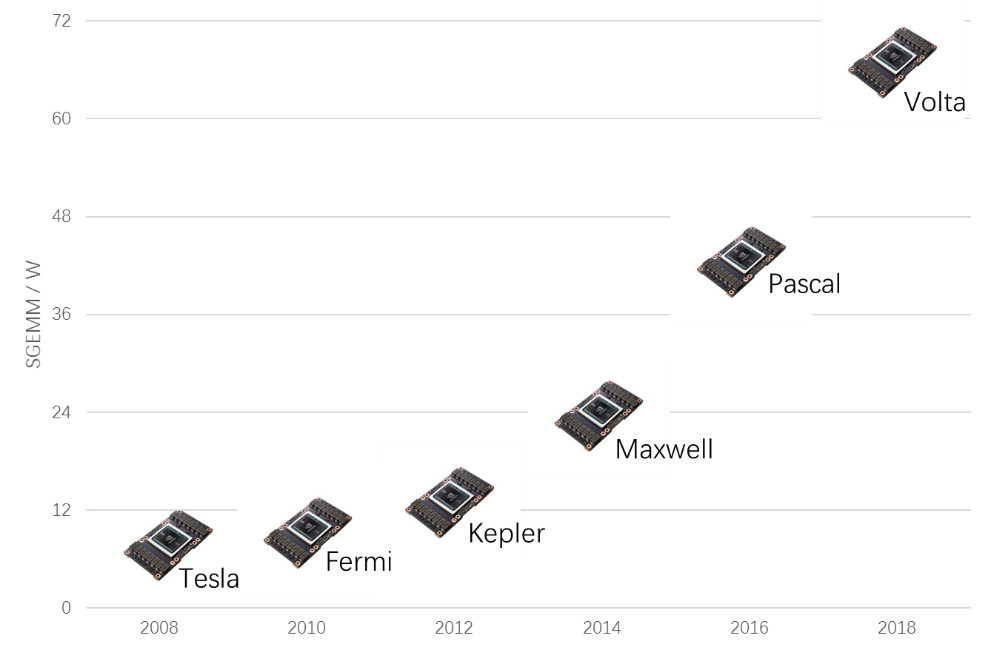
\includegraphics[width=0.40\textwidth]{nvidia_roadmap}
	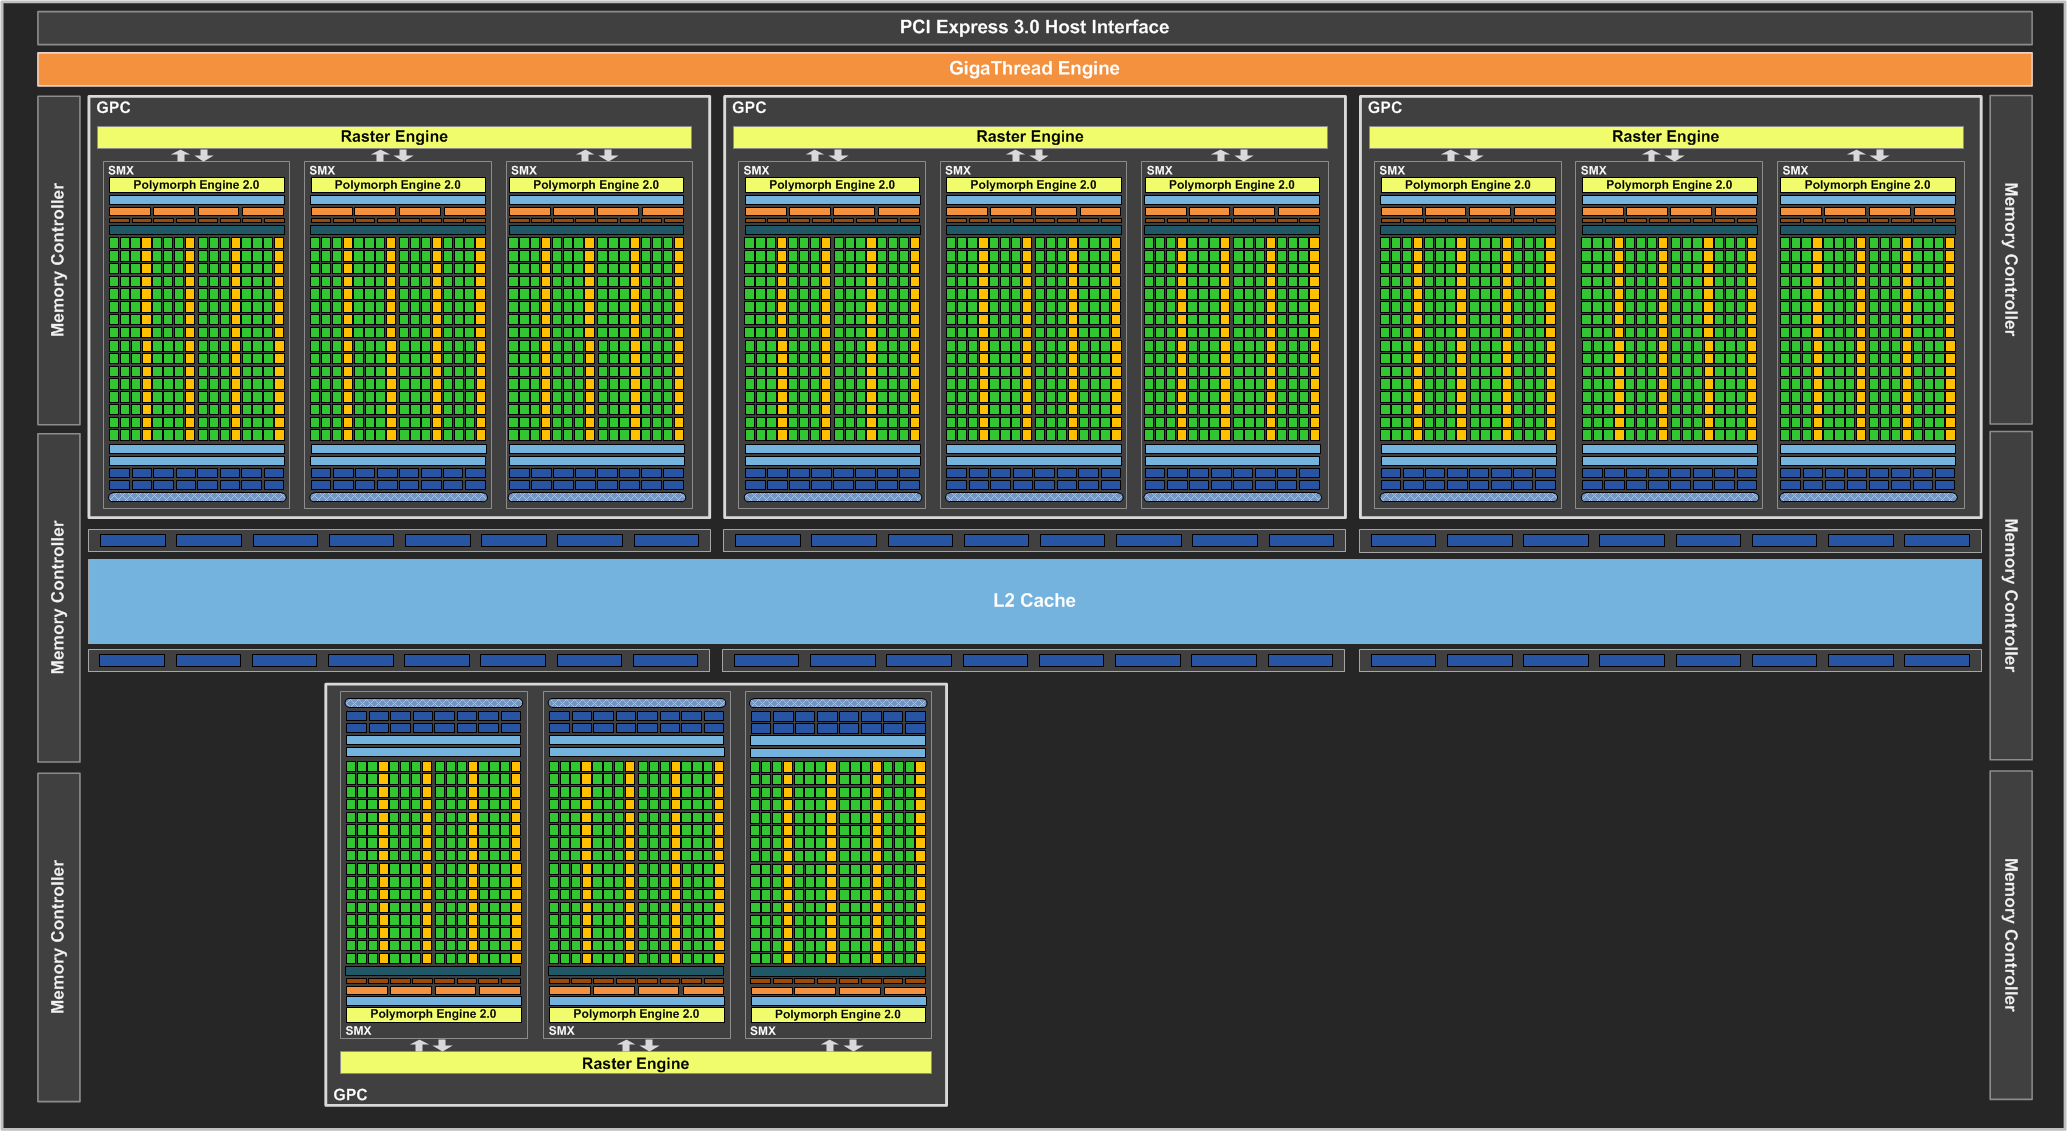
\includegraphics[width=0.50\textwidth]{nvidia_gtx780}
	\bicaption{NVIDIA GeForce GTX 780结构图}{NVIDIA GTX780 architecture}
	\label{fig:nvidia_gtx780}
\end{figure}

\begin{figure}[htbp]
	\centering
	%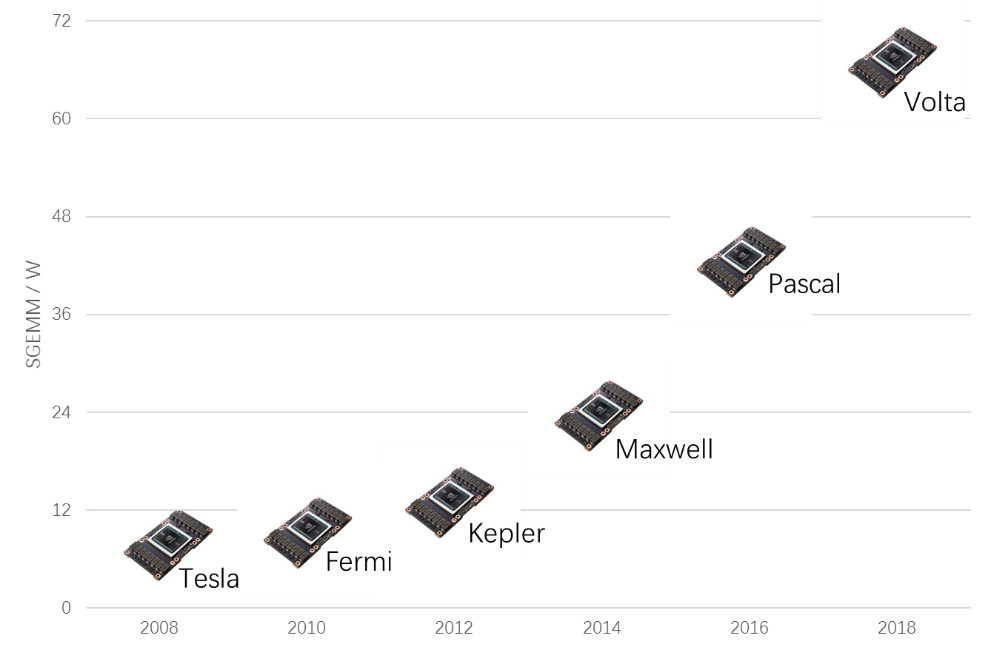
\includegraphics[width=0.40\textwidth]{nvidia_roadmap}
	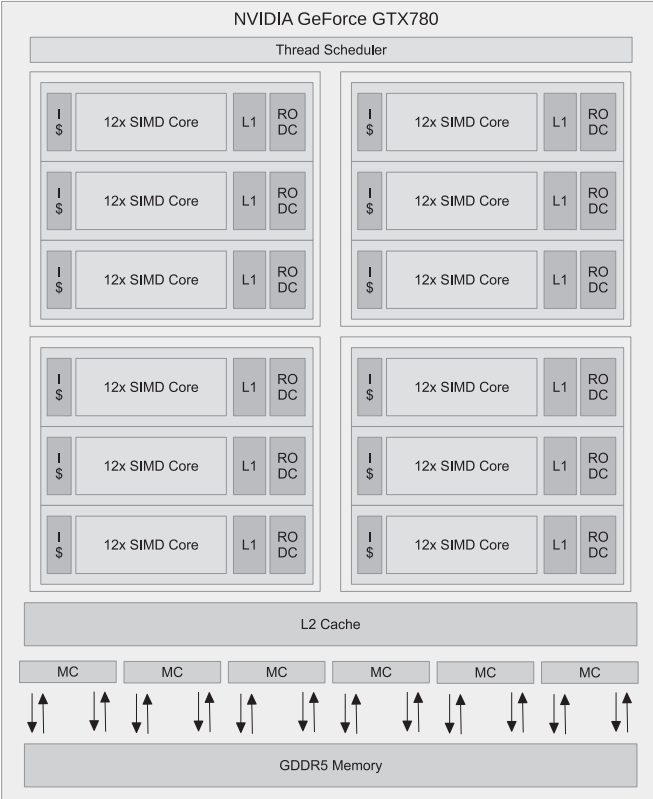
\includegraphics[width=0.50\textwidth]{nvidia_gtx780_simd}
	\bicaption{SIMD的角度看的GTX780结构图}{Structure of GTX780 from the perspective of SIMD}
	\label{fig:nvidia_gtx780_simd}
\end{figure}

SoCs在嵌入式领域已经应用了很多年,如数码相机,机顶盒和智能手机等应用场景。当前,SoCs开始走向桌面端。这种SoCs通常包含CPU和GPU,外加视频解码器,加密电路等部件。这种融合处理器广泛应用在笔记本,网络本和桌面端市场。AMD称这种SoCs为APU。可以看出,SOCs的出现是为了在满足性能要求的条件下,尽可能做到更低功耗和更低成本。将CPU和GPU融合在一个芯片的另外一个好处是,可以提高数据在CPU和GPU之间的周转速度,合适运行CPU和GPU之间通信为瓶颈的算法。


\section{本章小结}
本章主要讨论了各种处理器体系结构的发展史,以及在体系结构设计时的各种权衡。现代的GPU架构也是从这些结构中一步步发展而来。像超标量,VLIW结构都是早期大型计算机中处理器设计所采用的技术。早期的AMD GPU也是采用VLIW结构。CPU也从单核发展为多核处理器。为了追求更高的性能,指令的执行方式从简单的顺序执行发展为流水线,超标量,多发射和乱序执行。为了增加GPU的可编程性,GPU从专用的做图形渲染发展成GPGPU。可以做通用计算。AMD和NVIDA在GPU设计上都采用了SIMD这种灵活的结构。我们可以称之为向量处理器。这种结构非常适合现在的面向通量的计算。其中深度学习计算时一个典型的面向通量计算的场景。因此,随着云计算和深度学习的应用越来越广泛,GPGPU将会有非常大市场。


\chapter{GPU微体系结构研究}\label{chap:GPUArch}
\section{OpenCL编程模型}

\subsection{OpenCL程序语言介绍}
OpenCL是一种异构并行编程语言,OpenCL标准最初由苹果公司提出,同时参与的公司有AMD,IBM,Qualcomm,Intel和NVIDIA。最后由Khronos Group进行标准化和发布。Khronos Group在2008年发布了OpenCL标准的第一版,OpenCL 1.0。OpenCL 1.0定义了主机端的编程接口和设备端的编写kernel的语言。OpenCL语言基于C语言发展而来。随后发布的OpenCL 1.1和1.2标准增加了OpenCL与OpenGL的互操作性。在2013年,正式发布了OpenCL 2.0标准。新标准在一定程度上简化了并行程序的开发。OpenCL的API在设计上就做的尽可能通用,以使其可以运行在不同的平台上;并且也足够底层,以使其可以在不同的平台上都可以获得较高的性能。

OpenCL程序在不同的平台具有可移植性,按照OpenCL标准编写的程序,可以在不同的硬件平台上运行。

用OpenCL C语言编写在OpenCL设备上运行程序。OpenCL C在C99的基础上发展而来。其设计的目标是可在不同的OpenCL硬件平台(如GPU、FPGA、DSP等)上编写并执行可数据并行的程序。同时OpenCL C也实现了一组原子和同步操作。虽然OpenCL API本身是基于C的API,但也可以绑定到其他语言,例如Python,C++,Java等。另外,很多专用的库如数学库,计算机视觉库)也都集成了OpenCL的实现,来提升异构系统的计算性能。

所以,我们可以看到OpenCL的目标是做通用并行计算。
OpenCL 标准包含4部分,分别是平台模型,执行模型,kernel编程模型和内存模型。

平台模型:在OpenCL平台模型中,有一个主机端和一到多个设备端。主机端用来协调OpenCL代码的执行,设备端执行kernel代码。平台模型提供了一个抽象的硬件设备模型。

执行模型:执行模型定义了主机端OpenCL环境的配置和kernel的调用。这里包括OpenCL执行环境的配置,主机端与设备端的交互配置和kernel并发模型的配置。并发模型定义了如何kernel的执行分解到的线程和线程块这样的并行粒度。

Kernel编程模型:描述了如何将并发模型映射到具体的物理设备
内存模型:描述了kernel执行时使用的抽象内存层次结构,而不管具体的物理内存结构。

一个x86 CPU和GPU构成了常见的OpenCL硬件环境。其中CPU作为主机端,GPU作为加速器。使用执行模型,我们在主机端对 kernel进行配置,指定kernel执行时的并行粒度,并向GPU发出执行kernel的命令。我们在给GPU端的数据分配内存时,按照内存模型中的抽象内存层次来进行分配。OpenCL运行时和驱动将抽象的内存区域映射到具体的物理内存层次中。最后,使用kernel编程模型,GPU创建硬件线程来执行kernel;GPU进行调度时,线程会映射到具体的计算单元来执行。

一个通用的OpenCL设备包含多个CUs(Compute Units),每个CU每个最终由多个ALUs构成。一个线程(或者SPMD(单程序多数据)kernel的一个执行实例)最终会执行在一个ALU上。

对于AMD Radeon Instinct MI25(Vega10)和AMD Radeon Instinct MI8(Fiji)架构的GPU,每颗芯片有64个CUs,对于AMD Radeon Instinct MI6(Polaris)架构,每颗芯片有32个CUs。其中,每个CU包含一个标量单元和四个向量单元。每个向量单元是一个宽度为16的向量ALU。这四个向量单元以SIMD的方式执行指令。在单个CU上可以同时执行多个wavefronts。
\begin{figure}[htbp]
	\centering
	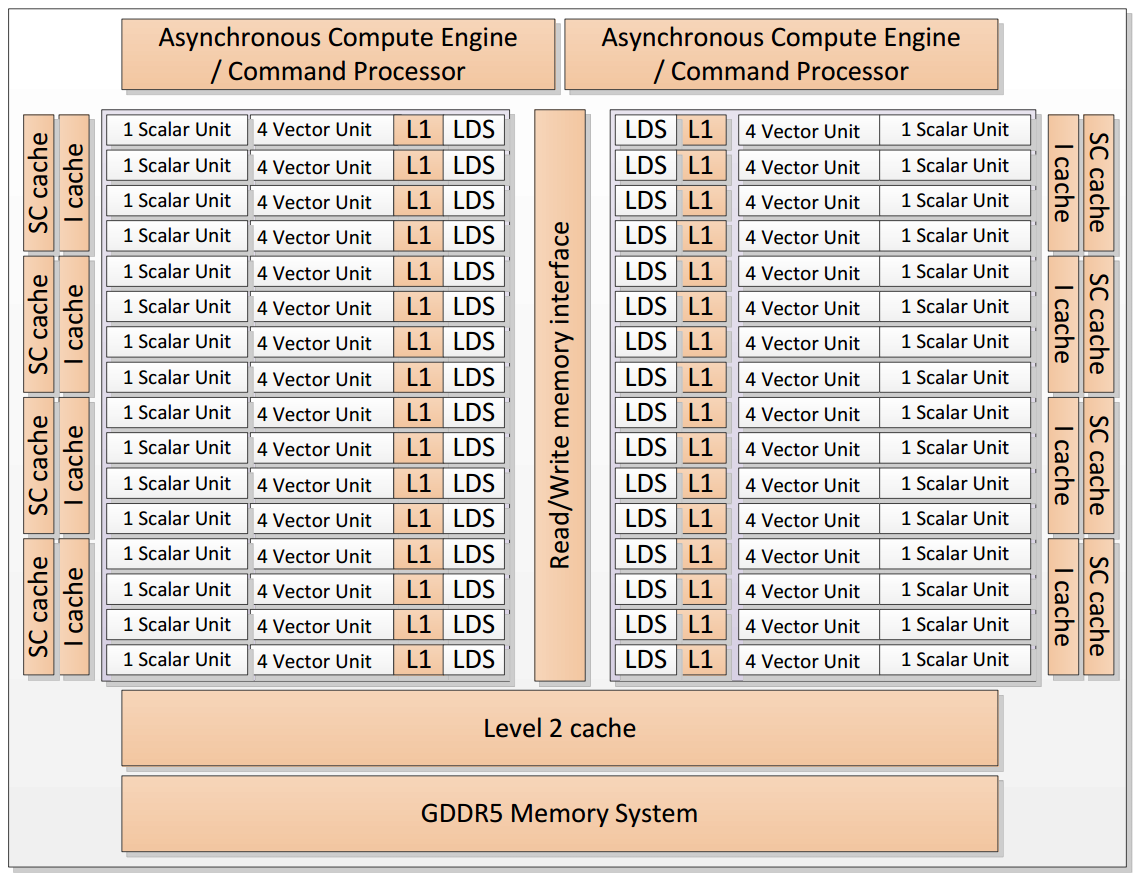
\includegraphics[width=0.50\textwidth]{gcn_gpu}
	\bicaption{GCN GPU结构图}{GCN GPU architecture}
	\label{fig:gcn_gpu}
\end{figure}
在AMD GCN架构中,一个CU包含一个标量单元和四个向量单元,一个L1 cache和一个LDS(Local Data Share)。在程序指令流中,既有标量指令也有向量指令。在每个时钟周期,指令调度器会选择一个标量指令和一个向量指令(或者访存指令,分支指令),分别发射到标量单元和向量单元。


\subsection{AMD ROCm软硬件系统}
本文主要针对AMD GPU架构做分析和性能调优。所以,我们就介绍AMD GPU的OpenCL实现。AMD APP(Accelerated Parallel Processing)是AMD最先提出的并行加速处理概念。AMD APP利用AMD GPU强大的处理能力来做高性能计算和数据并行处理。AMD ROCm系统包含AMD GPU、AMD多核CPU和与之相关的软件栈。

下图是AMD ROCm编译工具链。
\begin{figure}[htbp]
	\centering
	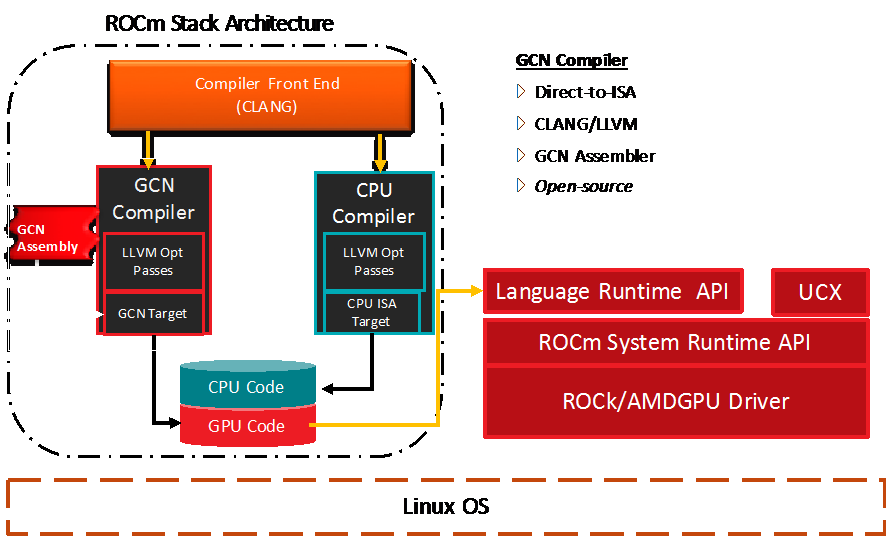
\includegraphics[width=0.50\textwidth]{rocm_llvm}
	\bicaption{AMD ROCm编译工具链}{AMD ROCm Compilation Tool Chain}
	\label{fig:rocm_llvm}
\end{figure}

AMD ROCm软件栈为用户和软件开发人员提供完整,灵活的软件开发工具来提升AMD GPU处理器的计算性能。AMD ROCm软件栈是一个开放的系统和一个标准的平台。AMD ROCm开放平台的策略让AMD的技术合作伙伴可以开发和提供第三方开发工具。

AMD ROCm提供的工具包括:
(1)  OpenCL编译器和运行时

(2)  调试和性能分析工具----AMD CodeXL

(3)  高性能数学库(rocBLAS, Tensile)---AMD加速并行处理数学库,用于优化NDRange特定算法

最新的AMD GPUs使用同一着色器架构可以在相同的硬件上交替运行不同的kernel。可编程GPU可以执行不同的用户程序,这些程序对图形编程人员称之为shaders,对于做通用计算的人称之为kernels。这些GPUs计算设备可以使用数据并行编程模型做通用计算,而不做图形渲染。AMD ROCM的编程模型将一组数据存放在内存中,这些数据可以被大量的计算单元(Compute Units)所访问。

\subsection{OpenCL线程模型}
Kernel的每个实例运行在Compute Unit(以下简称CU)上,称为work-item。work-items被映射到一个N维的索引空间,称为NDRange。
下面是AMD OpenCL线程模型和线程到CU的映射关系图示:
\begin{figure}[htbp]
	\centering
	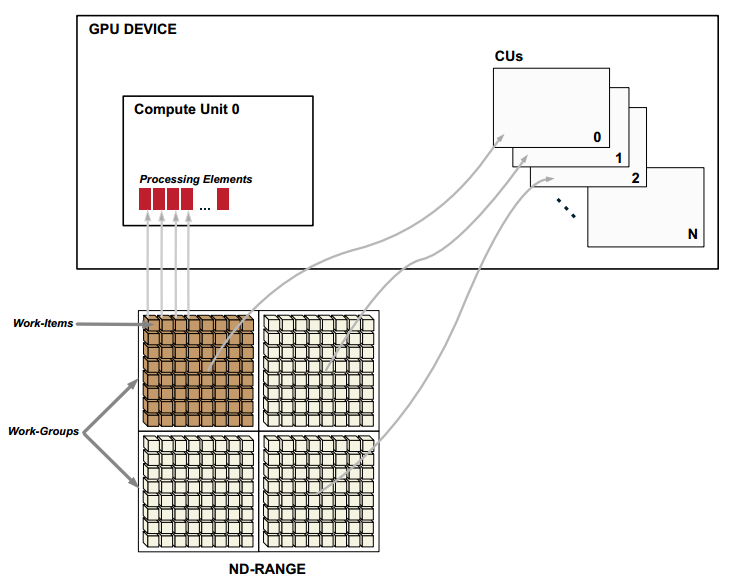
\includegraphics[width=0.50\textwidth]{opencl_thread_model}
	\bicaption{AMD OpenCL线程模型}{AMD OpenCL thread model}
	\label{fig:opencl_thread_model}
\end{figure}

一个work-group被分发到某一个CU上。Work-group中的work-item被一个CU中PE(Processing Element)所处理。一个PE在同一时刻只能处理一个work-item;但一个CU可以处理多个work-group。

OpenCL将所有要发射的线程映射到一个N维的索引空间。软件开发人员可以设定如何将work-items划分到work-group中。AMD GPU硬件调度的基本单元是wavefront,一个wavefront有64个线程(work-items)。一个work-group由整数倍个wavefront构成。

下面是work-item,wavefront和NDRange之间的映射关系图示:
\begin{figure}[htbp]
	\centering
	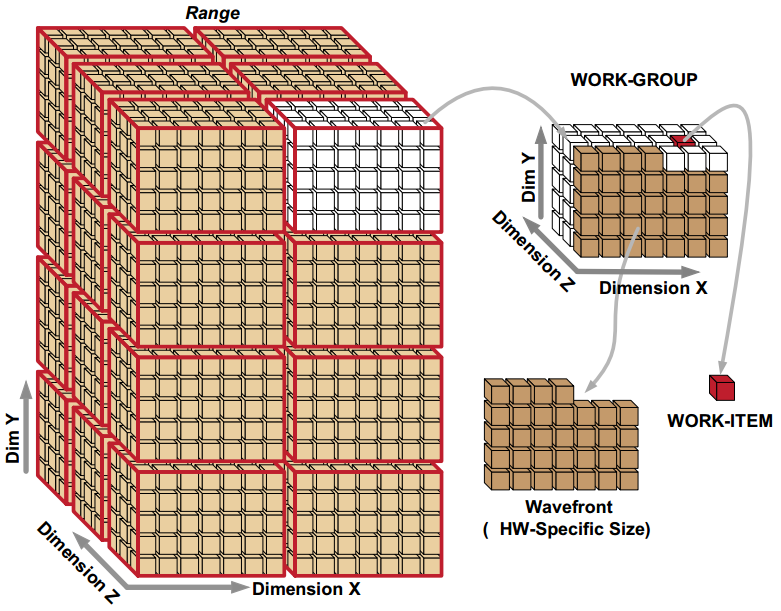
\includegraphics[width=0.50\textwidth]{thread_model}
	\bicaption{OpenCL线程组织方式}{OpenCL thread organization}
	\label{fig:thread_model}
\end{figure}

其中,wavefront是硬件上的概念,即AMD GPU硬件设计上的64个线程为一个基本调度单元。Work-group和NDRange是编写程序时的逻辑概念。

一个work-item在每个时钟周期会发射一条指令。多个work-item构成一个wavefront,作为一个基本调度单元。一个wavefront中至多有4个work-item组成流水线执行,来隐藏访存和计算延迟。例如,AMD GCN架构的GPU的实际处理宽度是16。每4个时钟周期发射一个宽度为64的指令。

wavefront拥有的线程数在不同系列的GPUs上会有不同。例如,一些低端GPUs,如AMD Radeon HD54XX系列的GPU,一个wavefront有32个线程。在更新的高端GPUs上,一个wavefront有64个线程。

每个CU的执行相互独立。所以,在不同的CU上,可以执行不同的指令。

下面讨论一下wavefront和work-group的关系。编程人员定义一个work-group,可以包含一到多个wavefronts。一个wavefront有自己的程序计数器(PC),所以每个wavefront都有自己的程序控制流。一个work-group包含的wavefront中的线程是线性排序的。例如,在64线程wavefront的GPUs上,线程0~63映射到wavefront0,线程64~127映射到wavefront1,按这样的顺序映射下去。为了充分利用硬件资源,我们要计算的数据个数最好是64的整数倍。

对于每个work-group,GPU会在单个CU上产生该work-group所需的wavefronts个数。如果一个wavefront中有非活跃的线程,那么这些线程所映射的GPU硬件计算核心将会空闲。出现这种情况的一个例子是我们的work-group的大小不是wavefront大小的整数倍。例如,如果一个work-group的大小是32,只使用了wavefront中的一半线程,那么就会有另外32个线程空闲。

在一个wavefront中,如果程序出现分支。Wavefront将会把有所的情况组合起来,顺序的执行。例如,一个wavefront中的一个分支包含两条路径,那么wavefront会先执行第一条路径,接下来执行第二条路径。分支的总执行时间是每个路径的执行时间的累加。例如,程序中有一个二分支结构,分支A和B,每个分支单独执行所需的时间都是t。只要wavefront中有一个线程在分支处和其他线程不同,那么整个wavefront执行完这段分支的时间就是2t。我们再举一个循环的例子,如果一个循环的单次执行时间是t。在一个wavefront中,有63个线程只执行这个循环的一次,另外一个线程执行该循环100次。那么整个wavefront执行完该循环的时间为100t。

编译和运行OpenCL程序,OpenCL编译工具链提供了一个可以同时编译CPUs和GPUs代码的通用框架。CPUs和GPUs代码共用编译器前端和部分高级的编译转换。编译器后端则针对不同的设备(CPU或GPU)做了专门的优化。

对于CPU,OpenCL运行时使用LLVM AS将代码编译成x86二进制代码。OpenCL运行时会自动确定CPU的核心数,并将OpenCL kernel交由核心执行。

对于GPU,OpenCL运行时对不完整的AMD IL做后处理,变成完整的AMD IL。这个过程会从宏定义库中添加针对特定GPU的宏定义。之后,OpenCL运行时会移除不必要的函数,将完整的IL代码交由着色器编译器,编译成针对特定GPU的二进制代码。
平台模型:

OpenCL平台包含一个主机端和一到多个OpenCL设备。一个OpenCL设备包含一到多个CUs(Compute Units),一个CU包含一到多个PEs(Processing Elements)。

平台模型是开发可在不同硬件平台上运行的程序的一个关键。在一个系统中,可能同时包含AMD GPU和NVIDIA GPU。

编程人员可以使用平台模型API来选择平台和计算设备。平台模型提供了一个抽象的设备体系结构,编程人员可以根据这个抽象体系结构来编写kernel。硬件厂商会将这个抽象体系结构映射到具体的物理硬件上。平台模型将设备定义为一组CUs(Compute Units),每个CU相对独立。每个CU由一组PEs(Processing Elements)组成。我们以2017年AMD新出Vega10架构为例,Vega10计算卡包含64个CUs,每个CU包含4个宽度为16的SIMD部件,所以一个CU的硬件向量宽度为64。我们可以计算出一张Vega10计算卡可以一次总共执行64x16x4=4096个指令。再根据Vega10的计算时钟频率最大为1.5GHz,每个时钟周期可以做2个浮点操作,我们可以计算出Vega10的理论单精度浮点峰值为64x16x4x2x1.5GHz=12288.0 Gflop/s。
获取平台和设备信息:

我们可以调用clGetPlatformIDs()函数来获取系统的平台信息。

获取了每个平台的ID号之后,我们通过调用clGetPlatformInfo()函数来获取每个平台的硬件厂商信息。

当我们选好平台后,接下来就可以调用clGetDeviceIDs()选择该平台的一个具体设备。

在本次实验中,我们的一个CPU连接两个AMD vega10 GPU。

我们接下来就可以选择在该平台每个设备的ID号后,可以通过调用clGetDeviceInfo()获取该平台每个设备的信息。

本次实验使用的是AMD vega10 GPU,又称gfx900。

对于vega10 GPU,有64个CUs。

更多信息在此就不一一列举。

前面部分主要介绍了如何获取选择平台和平台上的设备,并获取平台和该平台上设备的信息。虽然看起来很冗长,但对我们理解OpenCL的平台模型很有帮助。

执行模型:
为了主机端可以向设备发送命令和数据,我们要创建一个context。

Context介绍:

在OpenCL中,context是一个抽象环境。在这个抽象环境中,我们可以协调kernel的执行和管理kernel的内存。并且可以对kernel的执行进行跟踪。

OpenCL运行时(runtime)使用contexts来管理各种对象,例如命令队列(command queues),内存,程序(program)和kernel等对象;并且使用contexts中指定的设备来运行kernel。

在OpenCL中,查询平台和设备信息,创建context的过程看起来很冗长。然而,当我们写好这些代码后,我们就可以在之后的项目中重用这部分代码。

命令队列(command-queues):

设备端执行任务的方式是,主机端向设备端发送命令(commands),设备根据该命令来执行任务。这里的命令(commands)包括执行kernel,数据传输,同步操作。

主机端请求设备端执行任务,需要通过命令队列(command-queues)这种通信机制。当我们选定设备,并且创建了与选定设备关联的context之后,我们需要针对选定的每一个设备创建一个与之对应的命令队列(command-queues)。每个命令队列只能和一个设备关联。因为一个context中可能关联多个设备。在当前的context中,主机端向具体某一个设备发送命令时,就需要一个与该设备关联的命令队列。
当主机端需要某一个设备执行某种操作时,主机端需要将相应的命令提交到对应的命令队列中。

事件(Events):

OpenCL中的事件是与命令的状态相关联的对象。命令队列中的命令会产生事件,其他命令在执行之前需要等待某个事件。
设备端队列(device-side enqueuing):

从另一个角度来看我们的异构计算平台。我们可以将之看成master-worker模型。在该模型中,主机端(master)发送命令给设备端(worker)。通过master-worker模型,主机端和设备端可以协作工作。然而,在很多情况下,特别是在运行有前后依赖的算法时,主机端并不能静态的确定向设备端分发的任务数。例如在组合优化中,搜索区域的大小可能会决定下次work-groups的数目。然而,搜索区域的大小只能从上一次的迭代中获知。在之前的OpenCL版本中,为了给下一次运行的kernel设置合适的并行粒度,需要设备端和主机端进行通信来确定。为了去除这样的通信要求和提高系统性能,OpenCL 2.0在执行模型中增加了设备端队列(device-side enqueuing)。
在设备端正在执行的kernel可以将另外一个kernel放入该设备端队列。在这种情形下,我们称正在执行的kernel为父kernel,放入设备端的kernel为子kernel。当父kernel和所有子kernel都已执行完,父kernel在被标记为已完成。但父kernel和子kernel的执行可以是异步的。

Kernels和OpenCL编程模型:

前面介绍的执行模型是为了管理OpenCL命令的执行。OpenCL命令用来描述数据的传输和kernel的执行。OpenCL kernel是OpenCL应用中实际在设备上执行的那部分程序。和CPU上的许多并发模型类似,OpenCL kernel在语法上看起来和标准的C函数类似。这里的主要区别是OpenCL kernel有一组额外的关键字和OpenCL kernels所实现的并发模型。   
当使用操作系统提供的线程接口编写并发程序时,我们需要考虑实际的可用物理资源(如CPU物理核数)。当我们创建的线程超过CPU硬件线程数时,就需要考虑线程创建、线程间切换所带来的开销。而当使用OpenCL编写并发程序时,我们经常需要考虑如何采用最好的并行粒度来编写并行程序。

在OpenCL中,并发的最小粒度是work-item。每个work-item执行kernel函数。在向量加这个例子中,我们将循环的每一次映射到一个work-item。然后,让OpenCL运行时(runtime)来产生要计算的元素一样多的work-items。OpenCL运行时将work-items映射到GPU具体硬件计算单元上。从概念上来看,这种并行方式非常类似于MapReduce中的map操作。Map操作具有其天然的并行性。也类似于OpenMP中对for循环进行数据并行。

下图是NDRange,work-group,work-item之间的对应关系
\begin{figure}[htbp]
	\centering
	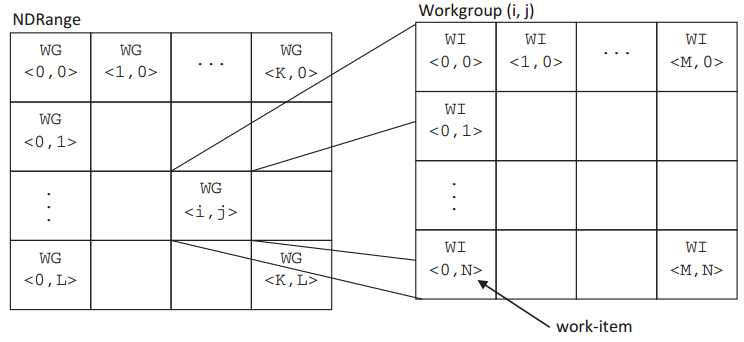
\includegraphics[width=0.50\textwidth]{thread_map}
	\bicaption{NDRange,work-group,work-item对应关系}{Relationship between NDRange, work-group and work-item}
	\label{fig:thread_map}
\end{figure}

在实际计算时,我们通常将NDRange映射到输入数据或者输出数据。在本文的矩阵乘实现中,我们将NDRange映射到输出数据,即C矩阵。

编译和参数处理:

一个OpenCL程序可能由多个OpenCL C kernel组成。例如,在代数求解器应用中,在一个OpenCL程序中可能包含向量加,矩阵乘和矩阵转置这几个kernel。在运行时(runtime)通过一系列API调用对OpenCL源程序进行编译。运行时(runtime)编译给系统提供了针对特定计算设备进行OpenCL kernel优化的可能,也让OpenCL kernel在之前未知的OpenCL兼容的设备上运行成为可能。由于OpenCL程序运行时(runtime)编译的特性,如果我们的OpenCL程序要在AMD,NVIDIA,Intel等这些硬件厂商提供的设备上运行时,我们不需要预先针对不同硬件平台进行预编译。

创建kernel的过程:

1.	OpenCL C源程序被存储在一个字符数组中。如果源程序存放在磁盘的文件中,则将其从磁盘读取到内存,并存放在一个字符数组中。

2.	通过调用clCreateProgramWithSource(),将OpenCL C源程序转化为程序对象 cl\_program 。

3.	通过调用clBuildProgram(),编译程序对象。

4.	通过调用clCreateKernel(),创建kernel对象cl\_kernel。

OpenCL kernel对象的具体二进制表示是和硬件厂商相关的。对于AMD运行时(runtime),主要有两种设备:x86CPU和GPUs。对于x86CPU,clBuildProgram()产生可以直接在x86CPU上执行的x86指令。对于GPU,则产生AMD GPU的中间表示语言,之后用just-in-time技术将中间语言编译成具体GPU指令集体系结构的二进制代码。

下图展示了OpenCL各种模型之间的关系。
\begin{figure}[htbp]
	\centering
	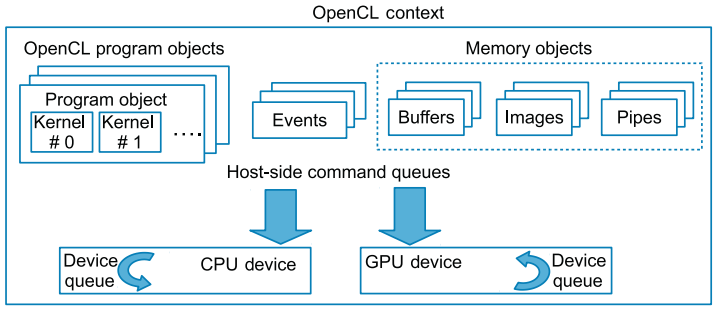
\includegraphics[width=0.50\textwidth]{opencl_model_relation}
	\bicaption{OpenCL模型之间的关系}{Relationship between OpenCL models}
	\label{fig:opencl_model_relation}
\end{figure}

NVIDIA也采用了类似的方法,将kernel代码首先编译成PTX(Parallel Thread eXecution)这种中间表示。这种中间表示的好处是可以让GPU ISA这样一代代演进,而不用考虑向后兼容的问题。因为GPU体系结构还处在一个非常快速的发展时期。

OpenCL内存模型:

不同计算设备的内存子系统会有很大不同。为了使得OpenCL代码具有可移植性,OpenCL定义了一个抽象的内存模型。编程人员可以基于该抽象内存模型来编写程序。不同的硬件厂商将此抽象内存模型映射到其具体设备的内存层次结构上。

对于OpenCL kernel来说,通常我们需要向kernel传入一些参数,kernel会输出一些参数。在kernel执行前,我们要将输入数据从主机端内存拷贝到设备端内存。为了将数据从主机端拷贝到设备端,我们需要将其封装成一个内存对象。同样,对于输出数据,我们也需要将其封装成一个内存对象。OpenCL定义了三种内存对象:buffer,images和pipes。在本文的矩阵乘中,用到buffers对象,所以我们主要介绍buffer内存对象。Buffer内存对象等价于C语言中我们用malloc()分配的数组空间。

OpenCL将内存分为两部分:主机端内存和设备端内存。主机端内存和设备端内存间的数据移动通过调用相应OpenCL API完成。

OpenCL设备端将内存分为4个区域。整个kernel可以访问的全局内存(Global memory)和常量内存(Constant memory),一个线程块可以访问的局部内存(Local memory),一个线程可以访问的私有内存(Private memory)。这几个内存区域在逻辑上是分离的,kernel开发人员可以显式的控制数据在这几个内存区域移动。

当我们将数据从主机端拷贝到设备端时,数据就拷贝到了设备端的全局内存。也只有设备端全局内存的数据的才可拷贝回主机端的主存。

局部内存通常映射到片上内存。片上内存相比全局内存延迟更低,带宽更高。每个线程的私有内存通常映射到寄存器中。

\begin{figure}[htbp]
	\centering
	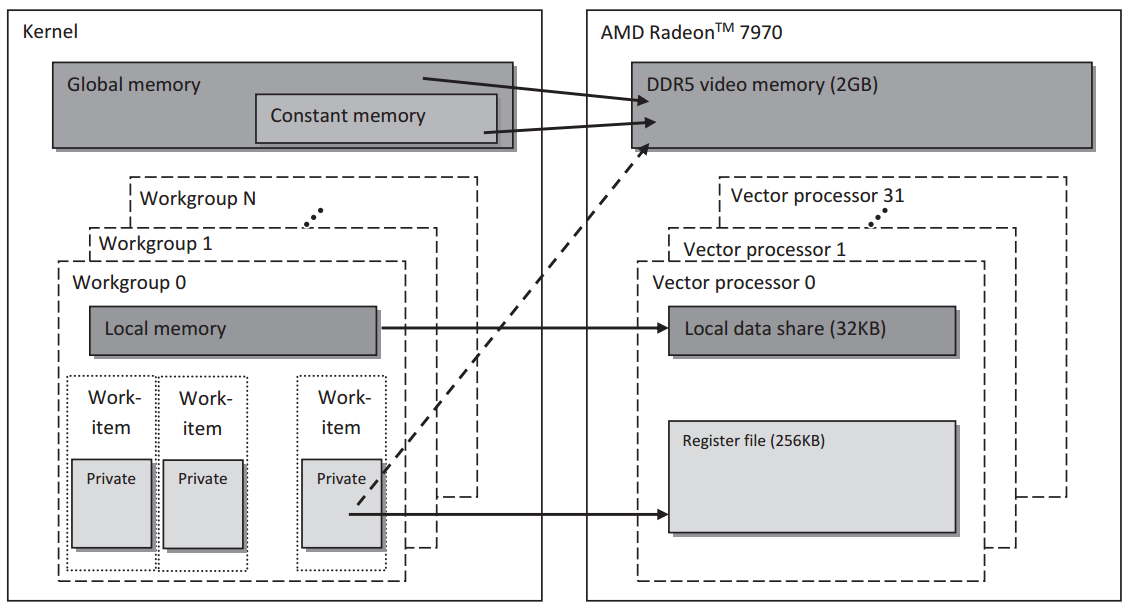
\includegraphics[width=0.50\textwidth]{opencl_memory_gpu}
	\bicaption{OpenCL模型中4种内存类型与AMD GPU内存的关系}{The relationship between four memory types in the OpenCL model and AMD GPU memory}
	\label{fig:opencl_memory_gpu}
\end{figure}

图中的虚线表示大部分情况下OpenCL中的线程私有内存对应到AMD GPU的寄存器。但也存在一些私有内存在溢出的情况下会对应到AMD GPU的片外内存。


\section{OpenCL程序在AMD GCN GPUs上的性能和调优}
我们现在来讨论AMD GCN(Graphics Core Next)架构GPUs上的程序性能和调优方法。AMD GCN架构的GPUs包括Fiji,Vega10和Vega20等。

\subsection{优化全局访存}
首先,我们先介绍一下GPU的组成结构。AMD GCN GPU由多个CU构成。每个CU包含局部内存(片上内存),L1 cache,寄存器和4个SIMD单元。每个SIMD包含16个计算核心。一个线程会在一个计算核心上执行,一个CU会运行一到多个work-groups。在GPUs上,硬件调度以wavefront 64个线程为基本调度单元,一个wavefront中64个线程执行相同的指令,但操作不同的数据。是一种典型的SIMD执行方式。

每个CU包含64KB的片上内存,16KB的读/写L1 cache,4个向量单元和1个标量单元。每个work-group可以最大分配32KB片上内存。每一个向量单元包含512个标量寄存器(SGPRs),用以处理一个wavefront中的分支,常量等操作。每个标量单元包含256个向量寄存器(VGPRs)。向量寄存器本质上也是标量寄存器,只是每个寄存器在长度上由1扩展到64。每个向量单元包含16个计算核心。

每个CU的L1 Cache为16KB,所以总的L1 Cache大小为15KB*(\# of CUs)。对于AMD Radeon HB7970 GPU,包含32个CUs,总共有512KB的L1 Cache。我们可以计算出L1的带宽为:

L1峰值带宽 = 

\#CUs*(4threads/clock)*(128 bits/thread)*(1byte/8bits)*Engine Clock

对于AMD Radeon HD7970 GPU,其理论峰值约为$\sim$1.9TB/s。

如果两个访存请求指向同一个内存控制器,在硬件上这两个请求会顺序执行。我们成为channel冲突。与之类似,如果两个访存请求映射到同一个内存bank,那么这两个请求也会顺序执行,我们称之为bank冲突。从软件开发人员的角度来看,channel冲突和bank冲突没有太大区别。如果数据请求的步长是2的幂次方的一个较大的数,那么往往会发生channel冲突。发生冲突的步长依赖于具体的芯片。如果一个步长在有8个channel的芯片上发生channel冲突,那么这个步长也可能会在有4个bank的芯片上导致bank冲突。

在本论文中,我们用bank冲突来统一指代channel冲突或bank冲突。

Channel冲突:

我们刚才讨论到,如果访存步长是一个较大的2的幂次方的一个数。那么往往会发生channel冲突。对于CPU来说,也会遇到同样的问题,访存步长为较大的2的幂次方的一个数,会使得访问的数据落在较少的Cache lines中,产生较多的cache不命中。

对于很多kernels来说,channel冲突对性能影响非常大。这时,我们就很有必要理解并解决channel冲突。

在GPU程序编写中,最好的方式是安排相邻的线程来读/写相邻的内存地址。这时一种避免channel冲突的方法。

当应用程序可以完全控制数据的访存模式时,软件开发人员就需要合理的组织数据结构,使得bank冲突最小化。

硬件地址字节分布:

\begin{figure}[htbp]
	\centering
	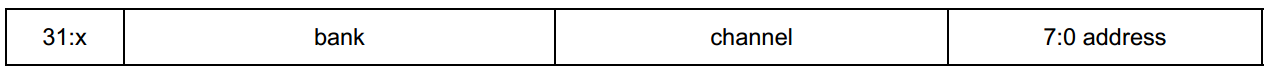
\includegraphics[width=0.50\textwidth]{gpu_addr}
	\bicaption{硬件地址字节分布}{Hardware address byte distribution}
	\label{fig:gpu_addr}
\end{figure}
Channel的计算方式:

if (({ row, bank} \%3) == 1)
channel\_within\_quadrant = 1

else

channel\_within\_quadrant = 2 * pipe[0]

下图是内存channel分布:
\begin{figure}[htbp]
	\centering
	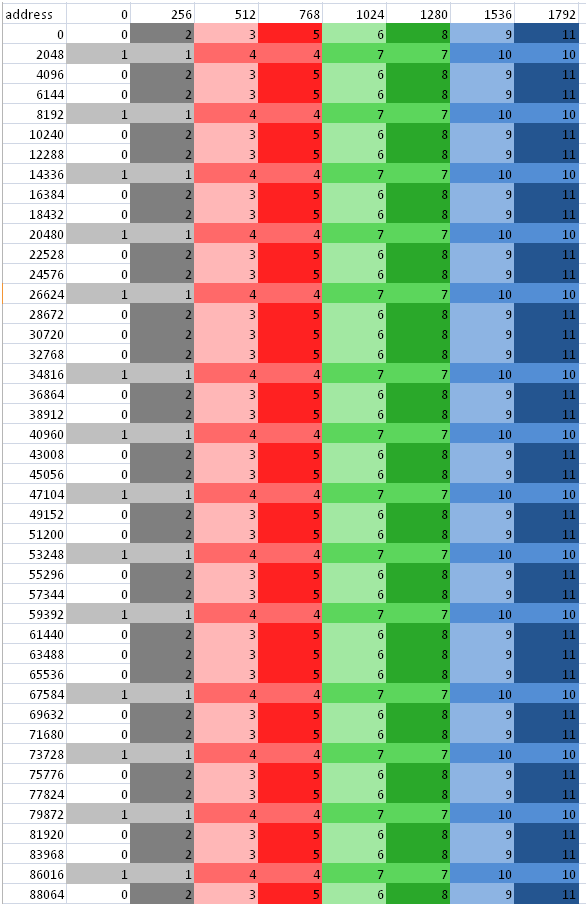
\includegraphics[width=0.50\textwidth]{gpu_mem_channel}
	\bicaption{AMD GPU channel分布}{AMD GPU memoyr channel distribution}
	\label{fig:gpu_mem_channel}
\end{figure}

我们可以从上图得到,如果我们访存步长是2048,那么我们将会有1/3的概率会访问到相同的channel;如果我们的访存步长是256,那么将会有1/6的概率访问相同的channel。

\section{GPU微体系结构}
\subsection{NVIDIA GPU架构}
NVIDIA GPUs由许多SMs(Streaming Multiprocessor)构成。每个SM包含多个SPs(Streaming Processor)(每个SP是基本的计算单元),调度器,和SFUs(Specital Functional Unit),LD/ST(Load/Store)单元,寄存器文件和统一共享内存/L1 cache。一个SM中的SPs共享寄存器文件和shared memory。NVIDIA GTX280,GTX580和GTX680三代GPU的比较(如图\ref{fig:nvidia_3_gpus})
\begin{figure}[htbp]
	\centering
	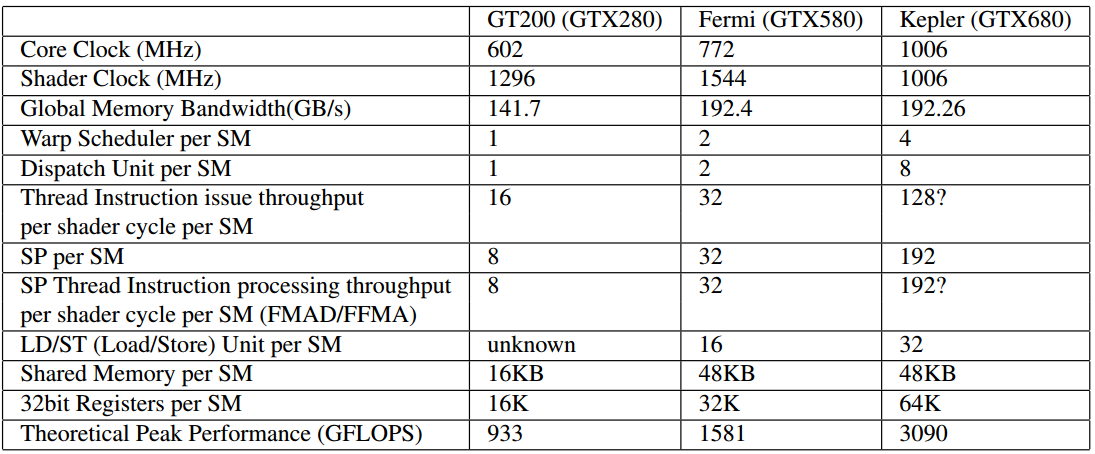
\includegraphics[width=0.50\textwidth]{nvidia_3_gpus}
	\bicaption{NVIDIA三代GPU的比较}{Comparison of NVIDIA Three Gen. GPUs}
	\label{fig:nvidia_3_gpus}
\end{figure}
从GT200到Kepler,SP(Streaming Processor)的数量急剧增长。从240(GTX280,65nm)到1536(GTX680,28nm)。然而,当我们从一个SP的角度来看,每个SP拥有的寄存器和shared memory这样的片上内存资源其实在变少。在Kepler(GTX680)之前的GPU,每个SM有两个时钟域:调度器的时钟core clock和SPs的时钟shader clock。Shader clock的频率大致是core clock的两倍。Kepler(GK104)之后,去掉了shader clock,一个SM的所有功能单元使用同一个时钟。为了便于比较不同的GPU架构,我们在Kepler GPU仍然沿用shader clock术语。

一个典型的CUDA程序通常会创建几千个并发线程来掩盖访存延迟和流水线延迟。线程的组织方式为,多个线程组成一个block,多个block再组成一个grid。一个Warp由32个线程组成,是SM上基本的执行和调度单元。我们将一个warp中所有线程执行的指令称为warp指令,将单个线程执行的指令称为thread指令。所以,一个warp指令包含32个thread指令。

在一个SM中,只有有限个线程可以并发的执行,称为active线程。一方面,一个SM中SPs越多,我们就需要更多的active线程来掩盖延迟。但另一方面,SM中的寄存器的数量和shared memory的大小等硬件资源又会限制SM中active线程的数量。从Fermi GPU到Kepler GPU每个SP可用的寄存器数量和shared memory大小在变少,因此单个SP支持的active线程数在减少。对于Fermi和Kepler GK104指令级,每个线程可用63个寄存器。因为在指令编码中,编码寄存器的段为6 bit。

\subsection{AMD GPU微架构}
 AMD GPU计算部件由多个Compute Unit(计算单元)组成,对应于NVIDIA的SM(Streaming Multi-processor), (从SIMD0~SIMD3)四个SIMD构成一个Compute Unit。每个SIMD有自己40-bit的程序计数器,和10个wavefronts(对应NVIDIA的warp)的指令缓存。一个Compute Unit(计算单元)可以最多可同时运行40个wavefronts,每个SIMD最多有10个wavefronts。Vega10 GPU增加了半精度浮点运算部件。



\subsubsection{AMD GCN Data Parellel Processor阵列结构}
 AMD GCN处理器实现了并行微架构,不仅为计算机图形应用提供了一个优秀的平台,而且也为通用数据并行应用提供了一个极好的平台。 任何需要高带宽或计算密集型的数据密集型应用程序都可以在AMD GCN处理器上运行。
GCN架构包括数据并行处理器(DPP)阵列,命令处理器,存储器控制器和其他逻辑。 GCN命令处理器读取主机写入系统内存地址空间中的内存映射GCN寄存器的命令。 当命令完成时,命令处理器将硬件生成的中断发送给主机。 GCN内存控制器可直接访问所有GCN设备内存和系统内存的主机指定区域。 为了满足读取和写入请求,存储器控制器执行直接存储器存取(DMA)控制器的功能,包括基于存储器中所请求数据的格式计算存储器地址偏移量。 在GCN环境中,一个完整的应用程序包括两部分:(1)在主处理器上运行的程序,以及(2)在GCN处理器上运行的程序,称为kernel。
下图展示了AMD Vega GPU内部结构
\begin{figure}[htbp]
	\centering
	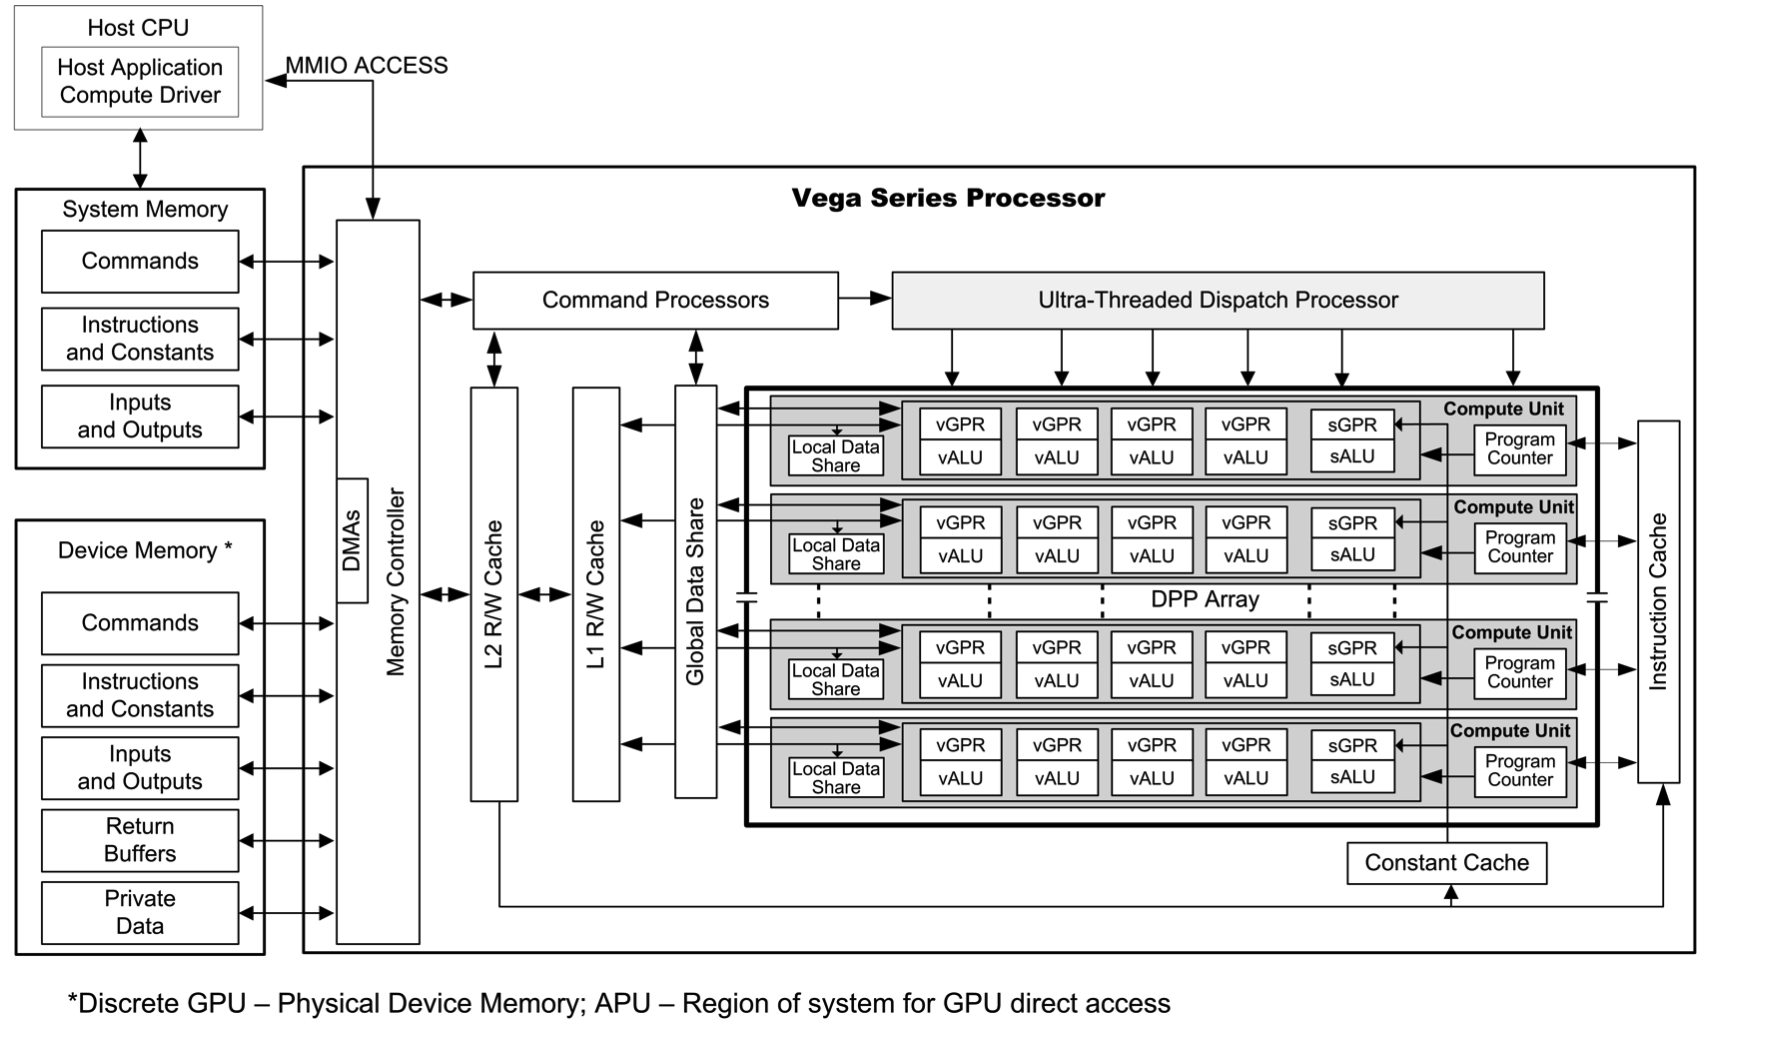
\includegraphics[width=0.50\textwidth]{amd_vega_arch}
	\bicaption{AMD VEGA GPU结构图}{AMD VEGA architecture}
	\label{fig:amd_vega_arch}
\end{figure}

GCN程序由主机命令控制,包括

(1)设置GCN内部基址和其他配置寄存器,

(2)指定GCN GPU要在其上运行的数据域,

(3)发送命令让GCN GPU开始执行程序。

GCN驱动程序在主机上运行。

DPP阵列是GCN处理器的核心。 该数组被组织为一组计算单元流水线,每个流水线独立于其他计算单元流水线,并行运行在浮点数据或整数数据流上。 计算单元流水线可以处理数据,或通过内存控制器将数据传输到内存或从内存传输数据。当DPP接收到一个请求时,计算单元管道从内存加载指令和数据,开始执行,直到内核结束。 内核正在运行时,GCN硬件会自动将指令从内存提取到片上高速缓存中; GCN软件在这方面没有任何作用。 GCN内核可以将数据从片外存储器加载到片上通用寄存器(GPR)和高速缓存中。

AMD GCN硬件可以检测浮点异常并生成中断。 特别是,他们在硬件中检测IEEE浮点异常; 这些可以被记录用于执行后分析。 上图中从命令处理器到主机的软件中断代表硬件生成的用于信号命令完成和相关管理功能的中断。GCN处理器通过跟踪潜在的数百个work-item的不同执行阶段,以及将计算操作与内存访问操作进行重叠来隐藏内存延迟。

下图显示了GCN应用程序的数据流。
\begin{figure}[htbp]
	\centering
	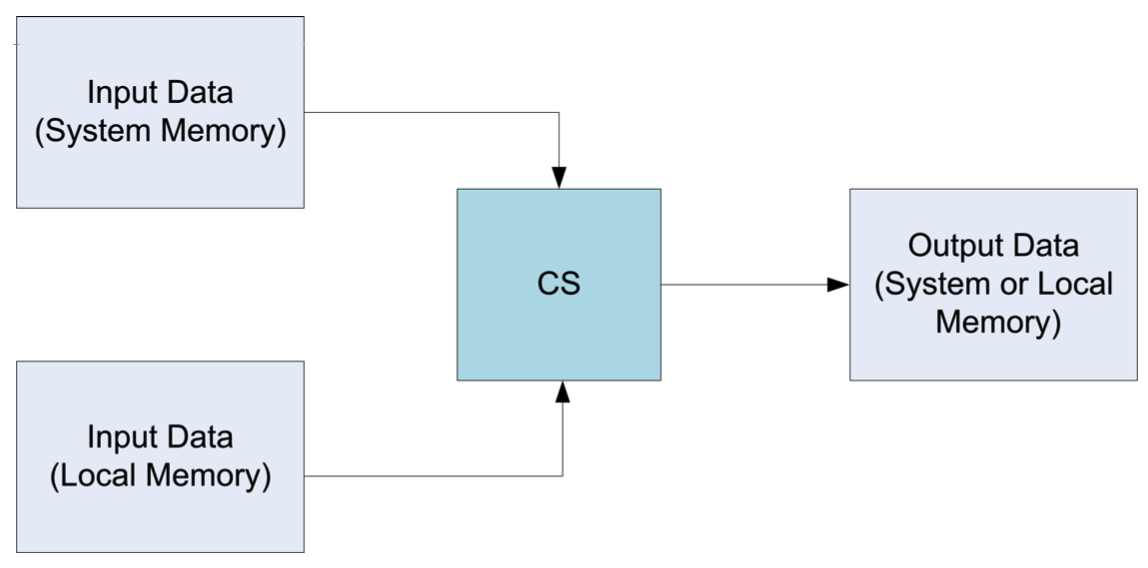
\includegraphics[width=0.50\textwidth]{amd_cs}
	\bicaption{GCN GPU程序数据流图}{GCN GPU program data flow diagram}
	\label{fig:amd_cs}
\end{figure}

GCN kernel是由GCN处理器执行的程序。从概念上讲,kernel在每个work-item上都是独立执行的,但实际上GCN处理器将64个work-item分组到一个wavefront中,wavefront一次执行所有64个work-itme上的kernel。

GCN处理器由以下部分组成:

•	一个标量ALU,对每个wavefront操作一个值(对所有work-itme通用)。

•	矢量ALU,它对每个work-item的唯一值进行操作。

•	Local Data Share允许workgroup中的work-itme进行通信和共享数据。

•	标量访存,可以通过Cache在SGPR和内存之间传输数据。

•	向量访存,可以在VGPR和存储器之间传输数据

所有内核控制流都使用标量ALU指令处理。这包括if / else,分支和循环。标量ALU(SALU)和访存指令适用于整个wavefront。向量访存和ALU指令一次对wavefront的所有work-itme进行操作。为了支持分支和条件执行,每个wavefront都有一个EXECUTE掩码,用于确定哪些work-item在当时处于活动状态,哪些处于休眠状态。活动的work-item执行矢量指令,休眠的工作项将该指令视为NOP。可以随时通过Scalar ALU指令更改EXEC掩码。向量访存指令在VGPR和存储器之间传输数据。每个work-item都提供自己的内存地址并提供或接收唯一的数据。这些也受到EXEC掩码的约束。

\subsubsection{AMD GPU内存层次结构}
AMD GCN流处理器可以在不同的work-item之间共享数据。 数据共享可以显着提升性能。下图展示了AMD GCN处理器内存层次结构。
\begin{figure}[htbp]
	\centering
	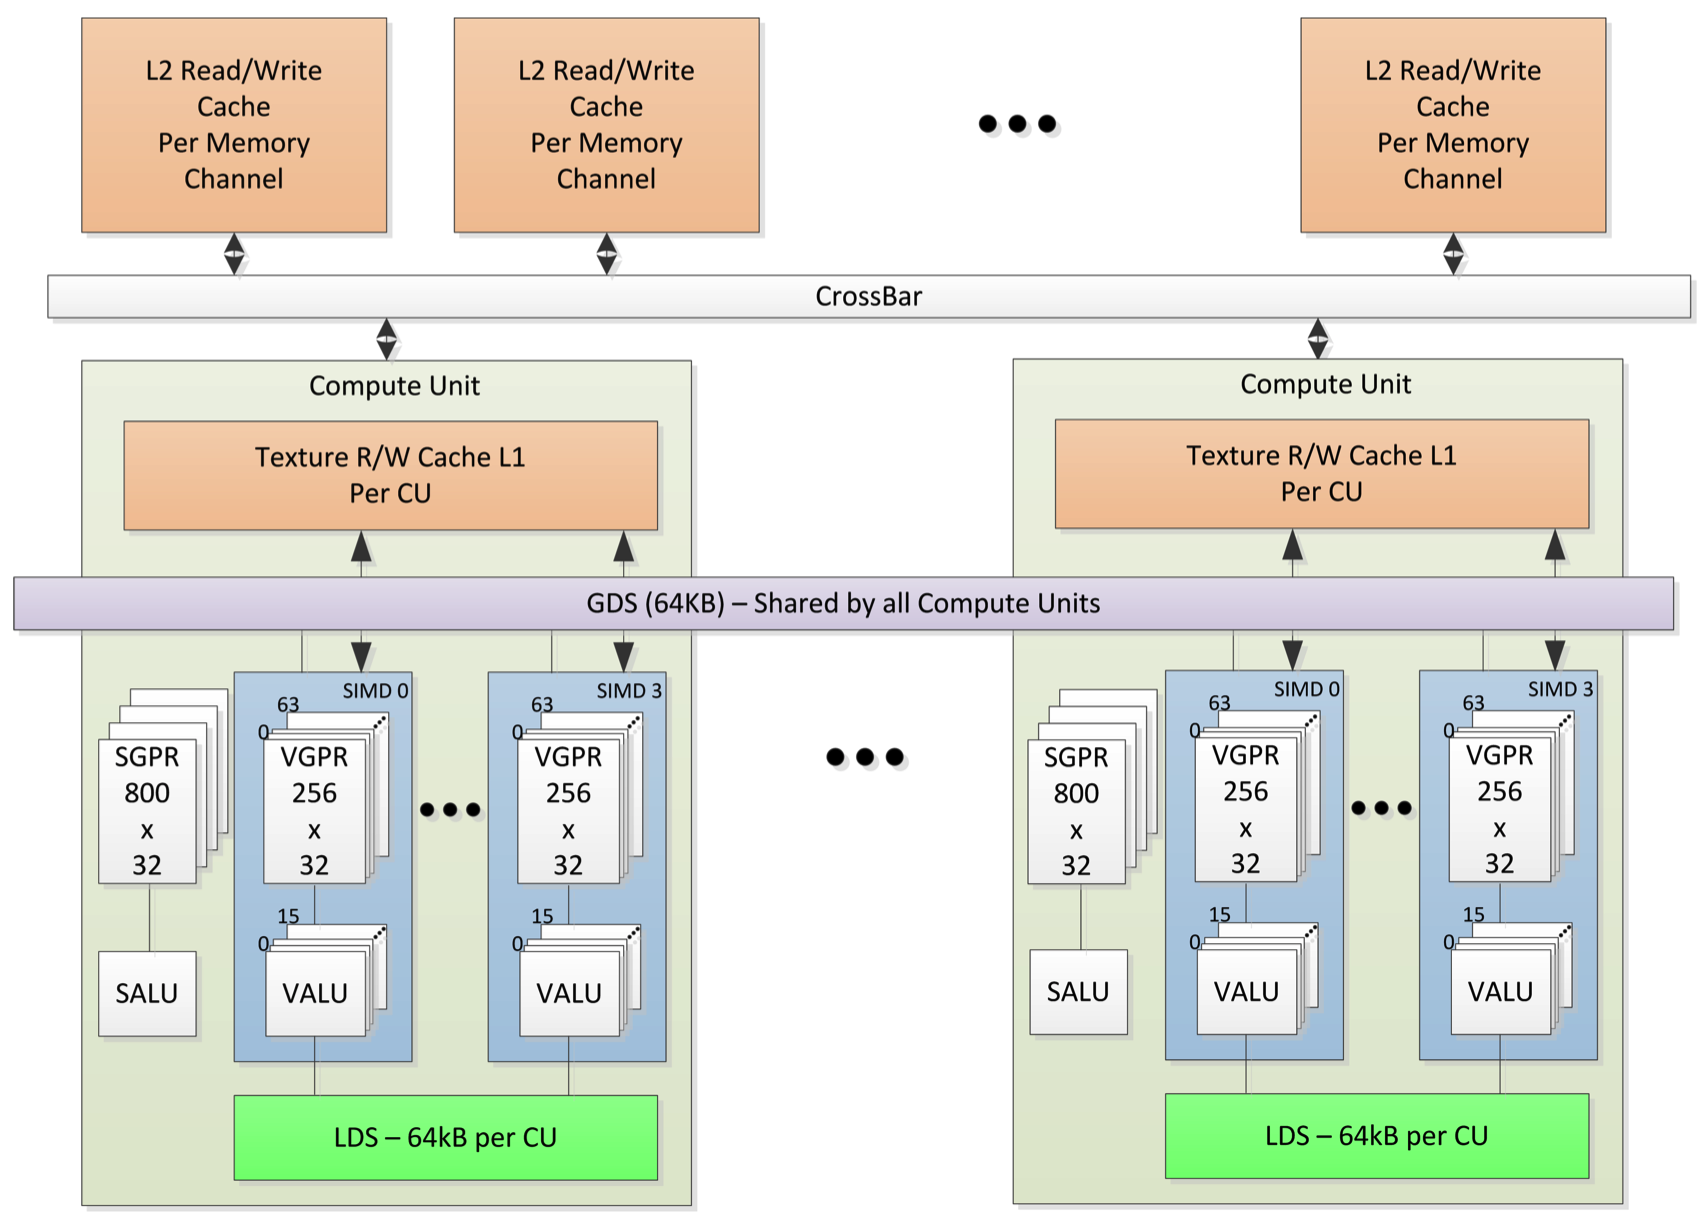
\includegraphics[width=0.50\textwidth]{amd_gpu_memory}
	\bicaption{AMD GPU内存层次结构}{AMD GPU memory hierarchy}
	\label{fig:amd_gpu_memory}
\end{figure}
每个CU都有一个64 kB的片上内存LDS(Local Data Share),可以实现一个work-group中不同work-item或一个wavefront中不同work-item之间的低延迟通信。每个LDS有32个banks,每个bank具有4个字节的512个条目。AMD GCN处理器为每个CU有64kB LDS; 这为CU提供了64kB的低延迟带宽。


\subsection{AMD GPU和NVIDIA GPU架构的比较}
在计算单元的设计上,AMD和NVIDIA GPU的计算单元都采用了SIMD(Single Instruction Multiple Data)或者SIMT(Single Instruction Mulitiple Thread)架构。在术语上,AMD称其为SIMD,NVIDIA称其为SIMT或SPMD(Single Program Multiple Data)。AMD GPU由很多CU(Compute Units)组成,NVIDIA GPU由很多SM(Streaming Multi-processors)或SMX组成。对于AMD Redeon Vega10架构,每个CU有4个SIMD部件,每个SIMD的宽度为16。通过向量流水线的方式用4个时钟周期来执行宽度为64的向量操作。对于NVIDIA GTX780,其设计为Kepler架构,每个SMX有12个SIMD,每个SIMD的宽度为16。通过2个时钟周期来执行宽度为32的向量操作。

对于AMD GPU GCN架构,每个CU包含一个标量部件和4个SIMD部件,每个SIMD最多可以有10个向量线程(AMD称为wavefronts)in flight,向量线程的宽度为64。一个SIMD在每个指令发射周期选择一个向量线程来执行。所以,一个CU最多可以运行40个向量线程。NVIDIA GPU在设计上也与之类似。但实际可运行的向量线程数受很多因素限制,这里包括寄存器数量,局部共享内存的大小等。

对于AMD GPU和NVIDIA GPU体系结构,采用了SIMD的编程模型,每个线程是SIMD中的一项。NVIDIA称之为“SIMT(Single Instruction, Multiple Thread)”或者“SPMD(Single Program, Multiple Data)”。对于AMD GPU,一个wavefront有一个程序计数器,指令的分支由专门的寄存器做掩码来标记,控制每个线程的行为。

通过上面的比较,我们可以看出,AMD GPU和NVIDIA GPU都采用了SIMD结构,不同的是AMD GPU所计算的向量的宽度为64,NVIDIA GPU所计算的向量宽度为32。由此可以窥见SIMD结构代表着现代GPU的主流设计方向。

对于AMD GPU GCN架构,每个CU包含一个标量部件和4个SIMD部件,每个SIMD最多可以有10个向量线程(AMD称为wavefronts)in flight,向量线程的宽度为64。一个SIMD在每个指令发射周期选择一个向量线程来执行。所以,一个CU最多可以运行40个向量线程。NVIDIA GPU在设计上也与之类似。但实际可运行的向量线程数受很多因素限制,这里包括寄存器数量,局部共享内存的大小等。

GPU上的指令级并行。对于AMD GPU每个时钟周期可发射多条向量指令,每个向量指令将被分发到不同的向量单元。AMD GPU的指令可以超标量执行,在同一个CU上,可以同时执行访存指令,计算指令和其他占用不同部件的操作。这样可以提高GPU执行指令的通量。AMD Radeon R9 290X有44个CUs,每个CU包含4个向量单元,共176个向量单元。NVIDIA GeForce GTX 780有12个SMX,每个SMX有12个向量单元,共144个向量单元。这两种GPU都有高速片上内存,在OpenCL的术语中,称之为局部内存。以一个线程块(work-group)为单位进行分配。

相比于CPU中线程的概念,GPU中的线程非常轻量级,可以做非常快速的线程切换。GPU大量轻量级线程的特点,使其可多任务快速切换和实现高吞吐量。线程的运行上,GPU会简单很多,是顺序发射,没有CPU中线程的多发射和乱序执行。由于GPU有大量向量部件,通过产生大量轻型线程来充分利用这些部件。所以,GPU是面向通量计算的处理器。




\section{AMD GPU微基准测试}
通过设计微基准测试程序,我们可以探测AMD GPU的指令通量和带宽。


\subsubsection{AMD GPU指令通量和带宽探测}
\begin{figure}[htbp]
	\centering
	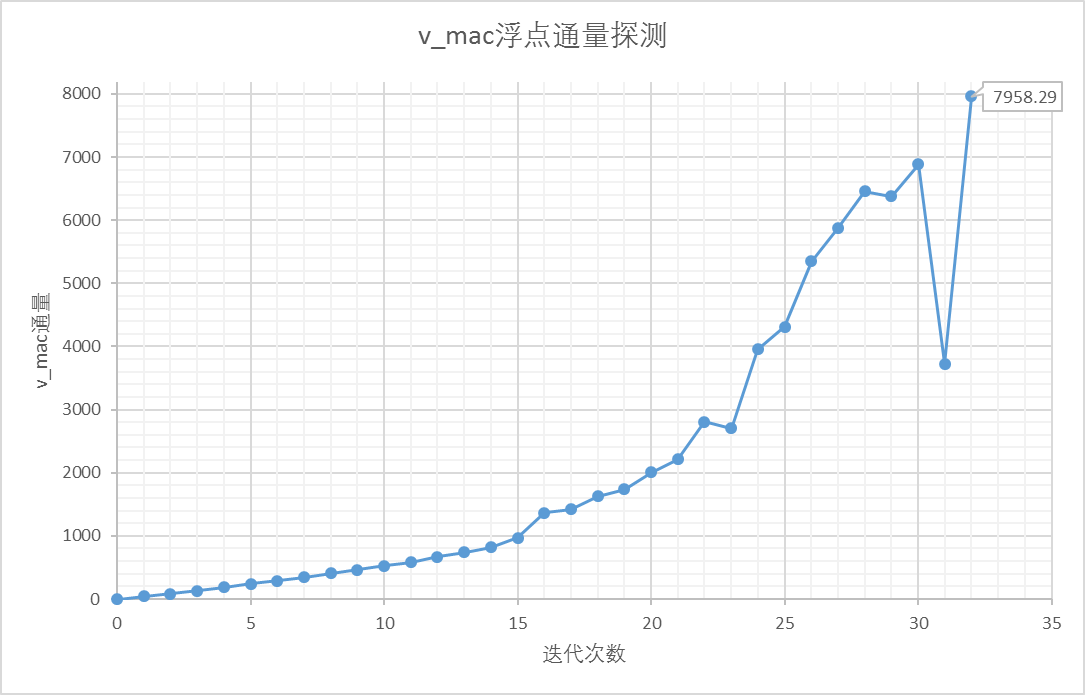
\includegraphics[width=0.50\textwidth]{v_mac_throughput}
	\bicaption{AMD Fiji GPU浮点通量测试}{AMD GPU memory hierarchy}
	\label{fig:v_mac_throughput}
\end{figure}

我们探测得的AMD Fiji R9 Nano GPU的浮点通量为7958.29gflop/s。Fiji GPU的理论浮点峰值为8192gflop/s,所以实测浮点性能为7958.29/8192 = 97.15\%。

\begin{figure}[htbp]
	\centering
	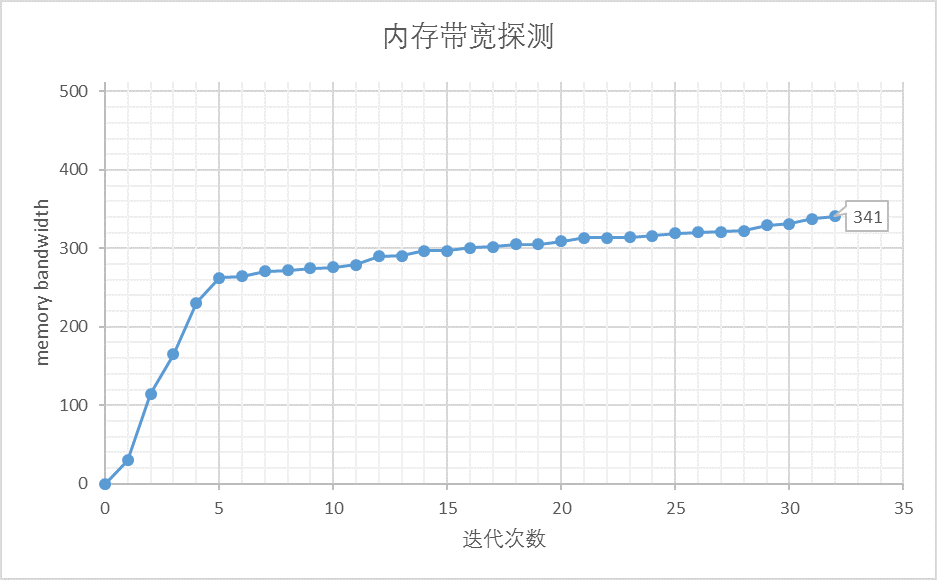
\includegraphics[width=0.50\textwidth]{mem_bandwidth}
	\bicaption{AMD Fiji GPU内存带宽测试}{AMD GPU memory hierarchy}
	\label{fig:mem_bandwidth}
\end{figure}

我们探测得的AMD Fiji R9 Nano GPU的内存带宽为341GB/s。Fiji GPU的理论内存带宽为512GB/s,所以实测浮点性能为341/512 = 66.6\%。



\section{本章小结}
本章从GPU体系结构和OpenCL编程模型两方面对GPU架构进行了详细的描述。并探测了AMD GPU的浮点指令通量和内存带宽,为后面矩阵乘GPU调优做铺垫。



\chapter{矩阵乘GPU实现}\label{chap:GEMMGPU}

%我们使用外积(outer product)法计算矩阵乘。因为外积法比內积法(inner product)在GPU上的并行性好。例如,我们要计算下面的矩阵乘法C=AxB。使用內积法,我们需要按照下面的公式计算:
本文使用外积(outer product)法计算矩阵乘。因为外积法比內积法(inner product)在GPU上的并行性好。例如,要计算下面的矩阵乘矩阵$C=A \times B$。使用內积法,需要按照下面的公式计算:

\begin{equation}
\label{eq:innerproduct}
C[i][j]=\sum_{k}A[i][k]B[k][j]
\end{equation}

%我们可以并行的计算所有的乘法,但不能并行的计算加法。即使我们可以使用reduction来快速计算加法,但仍然会产生很多空闲的线程。这样,由于任务划分的不均衡,会使得计算性能大大降低。然而,如果我们用外积法来代替內积法,将会很大程度上缓解负载不均衡带来的性能损失。下面是外积法的计算公式:
采用內积法可以并行的计算所有的乘法,但不能并行地计算加法。即使可以使用reduction来快速计算加法,但仍然会产生很多空闲的线程。这样,由于任务划分的不均衡,会使得计算性能大大降低。然而,如果用外积法来代替內积法,将会很大程度上缓解负载不均衡带来的性能损失。下面是外积法的计算公式:

\begin{equation}
\label{eq:outerproduct}
C^{(k)}=A[:][k]B[k][:], C=\sum_{k}C^{(k)}
\end{equation}

在计算A[:][k]B[k][:]时,每个线程只需负责读取A的一个小块和B的一个小块,来计算对应C的一个小块;每个线程可以独立的将当前计算得到的C的一小块的部分和累加到对应C的一小块上。当C的部分和全部都累加起来时,我们一次性写回C到全局内存。

%在算法设计上,我们采用外积法, A矩阵列优先存储,B矩阵行优先存储, 图\ref{fig:outer_product}为一个block中的线程读取A,B中的数据块, 和对应到C矩阵的输出
在算法设计上,本文采用外积法, A矩阵列优先存储,B矩阵行优先存储, 图\ref{fig:outer_product}为一个block中的线程读取A,B中的数据块, 和对应到C矩阵的输出。

%问题定义: C = A * B, A大小为MxK, B为KxN, C为MxN 
问题定义: $C = A * B$, A大小为$M \times K$, B为$K \times N$, C为$M \times N$

矩阵乘外积法:用A矩阵的一列乘以B矩阵的一行,沿着K方向做累加,可以计算出结果C(图\ref{fig:outer_product})。
\begin{figure}[htbp]
	\centering
	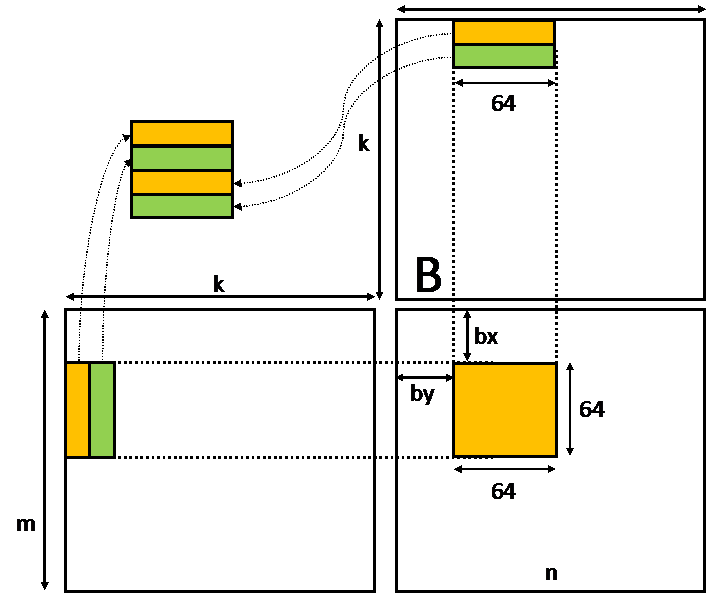
\includegraphics[width=0.50\textwidth]{outer_product}
	\bicaption{矩阵乘外积法图示}{Illustration of Outer-product matrix multiplication method}
	\label{fig:outer_product}
\end{figure}
\section{矩阵乘外积法算法描述}

%\begin{algorithm}[htbp]
%	\small
%	\caption{GEMM algorithm}\label{alg:gemm}
%	\begin{algorithmic}[1]
%		%\Procedure{Euclid}{$a,b$}\Comment{The g.c.d. of a and b}
%		\State preload block of A, B
%		\While{one more valid block of A, B exists}
%		\State load block of A, B from global memory to registers
%		\State store block of A, B from registers to shared memory
%		\State load block of A, B from shared memory to registers
%		\State compute block of C in registers
%		\EndWhile\label{gemmendwhile}
%		\State store C from registers to global memory
%		%\EndProcedure
%	\end{algorithmic}
%\end{algorithm}

\begin{algorithm}[htbp]
	\small
	\caption{GEMM algorithm}\label{alg:gemm}
	\begin{algorithmic}[1]
		%\Procedure{Euclid}{$a,b$}\Comment{The g.c.d. of a and b}
		\State $A, B, C$\Comment{matrix A, B, C}
		\State $regA[task\_size],regB[task\_size],regC[task\_size]$\Comment{Allocate register for compute}
		\State $tileA[tile\_size],tileB[tile\_size]$\Comment{Allocate shared memory for tile of A, B}
		\State $regC \gets 0$
		\While{one more valid block of A, B exists}
%		\State load block of A, B from global memory to registers
%		\State store block of A, B from registers to shared memory
%		\State load block of A, B from shared memory to registers
%		\State compute block of C in registers
        \State $tileA \gets A, tileB \gets B $\Comment{Load tile of A, B from global to shared}
        \State barrier
        \For   {$k = 0$; $k<NUM\_UNROLL$;$++k$}\Comment{Loop Unroll}
        \State $regA \gets tileA, regB \gets tileB$
        \State $regC += regA \cdot regB$
        \EndFor
        \State barrier
		\EndWhile\label{gemmendwhile}
		\State $C \gets regC$\Comment{Store C from registers to global memory}
		%\EndProcedure
	\end{algorithmic}
\end{algorithm}

在算法\ref{alg:gemm}执行上,我们经过下面的步骤:

(1)	数据预取,从全局内存读取A,B矩阵数据块到寄存器。

(2) 循环开始:

\qquad(2.1) 从全局内存读取A,B数据块到寄存器。

\qquad(2.2) 将读取到寄存器的数据写回的共享内存。

\qquad(2.3) 从共享内存读取A,B数据块到寄存器。

\qquad(2.4) 在寄存器中计算结果C。

\qquad 直到所有的A,B数据块都读取完。

(3) 最后把C的结果从寄存器写回到全局内存。


\section{从全局内存读取数据到共享内存}
全局内存是对所有线程可见,共享内存是对一个线程块里的线程是可见的,寄存器是对线程私有的。从全局内存读取数据到寄存器,然后到共享内存,是为了通过数据分享共享内存的数据,减少慢速的全局内存的访问次数,改为共享内存的访问。展示了线程块从矩阵A和B读取数据到共享内存的过程。线程块分别从矩阵A和矩阵B读取bmxbk和bkxbn的数据,然后使用外积法计算。为了隐藏全局访存的延迟,我们采用软流水和共享内存双缓冲机制。共享分块的大小与GPU上的计算资源如寄存器大小和共享内存大小有关。由于指令不能直接从全局访存读取到共享内存,需要寄存器中转,因此需要分两个步骤。

\subsection{线程到数据的映射}

\begin{figure}[htbp]
	\centering
	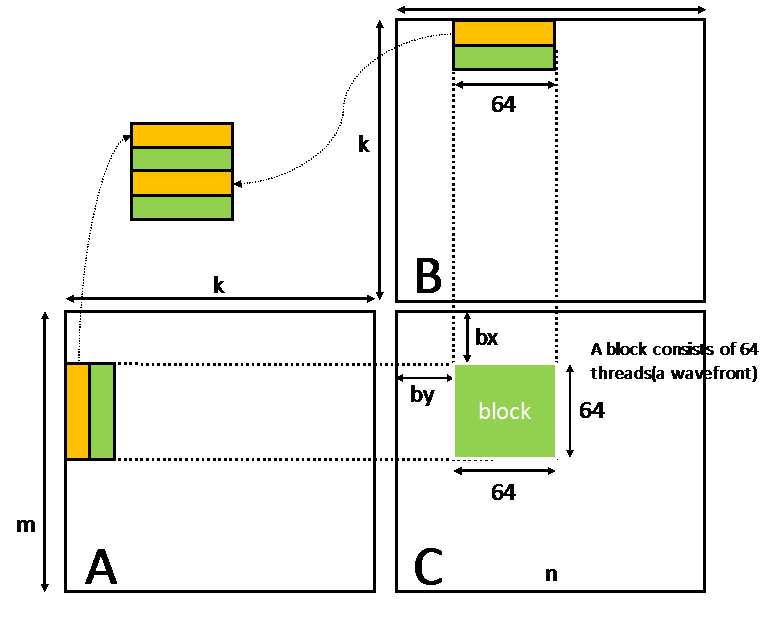
\includegraphics[width=0.50\textwidth]{thread_to_data}
	\bicaption{线程到数据映射}{Thread-to-data mapping}
	\label{fig:thread_to_data}
\end{figure}

64个线程(即一个wavefront)组成一个block,每个线程计算8x8的输出,一个block共计算64x8x8=64x64的输出(如图\ref{fig:thread_to_data})。

\begin{figure}[htbp]
	\centering
	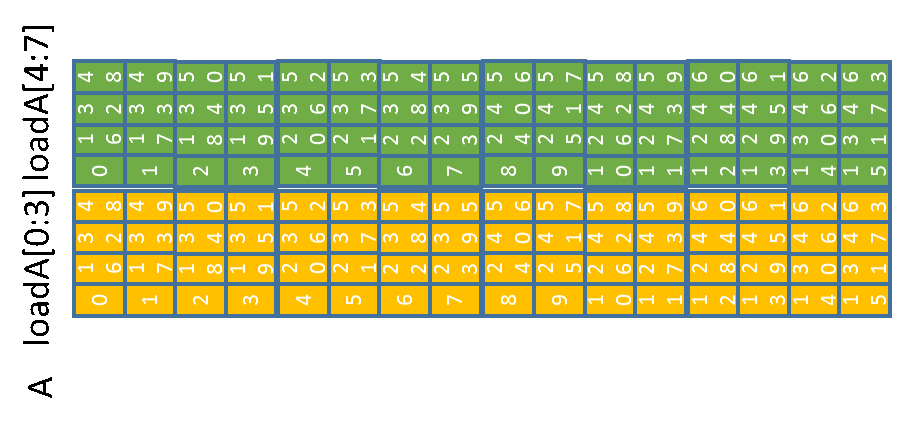
\includegraphics[width=0.50\textwidth]{global_A}
	\bicaption{从全局内存读取A矩阵数据到寄存器}{Read A-matrix data from global memory to registers}
	\label{fig:global_A}
\end{figure}

\begin{figure}[htbp]
	\centering
	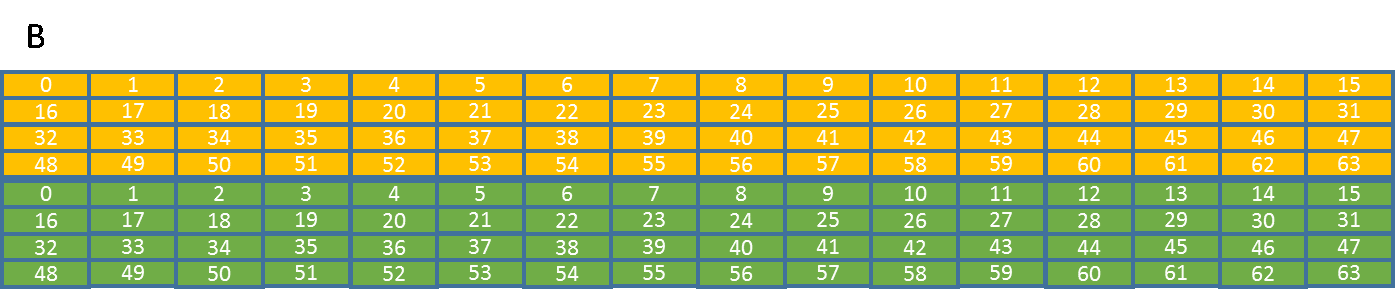
\includegraphics[width=0.50\textwidth]{global_B}
	\bicaption{从全局内存读取B矩阵数据到寄存器}{Read B-matrix data from global memory to registers}
	\label{fig:global_B}
\end{figure}

A(表示保存A矩阵数据的寄存器) : 从全局内存读A数据到寄存器(如图\ref{fig:global_A})

B(表示保存B矩阵数据的寄存器) : 从全局内存读B数据到寄存器(如图\ref{fig:global_B})

图中,小方格中的数字表示threadblock中的线程号。黄色表示已经把全局内存中的数据加载到了寄存器,绿色表示下一次计算需要用到的数据(还没加载好)。黄色和绿色构成寄存器双缓冲。

\begin{figure}[htbp]
	\centering
	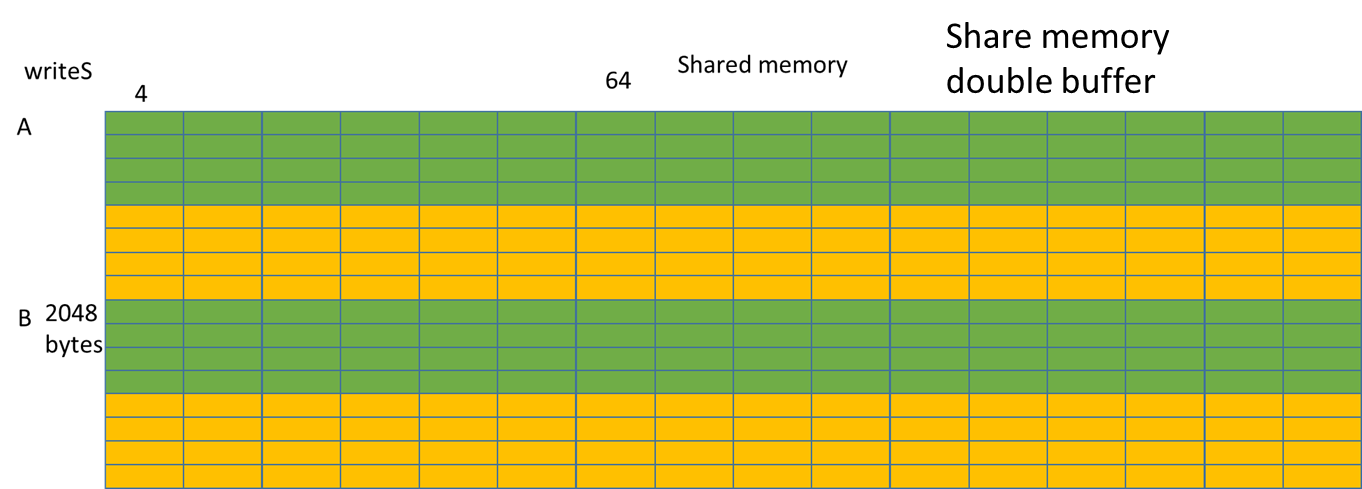
\includegraphics[width=0.50\textwidth]{writeS}
	\bicaption{写回A,B数据到共享内存}{Write A,B to shared memory}
	\label{fig:writeS}
\end{figure}

将寄存器中读好的A,B写回到局部共享内存。图\ref{fig:writeS}中绿色表示正在从寄存器写回数据到局部共享内存,黄色表示下一次要写回到局部共享内存的地址。黄色和绿色构成局部共享内存双缓冲。


\section{从共享内存读取数据到寄存器并计算}
矩阵A,B是否转置只与读取全局内存有关,一旦数据存储到共享内存,访问无关。所以从此步骤之后,论述任务划分时,不再区分矩阵A,B是否转置。
\begin{figure}[htbp]
	\centering
	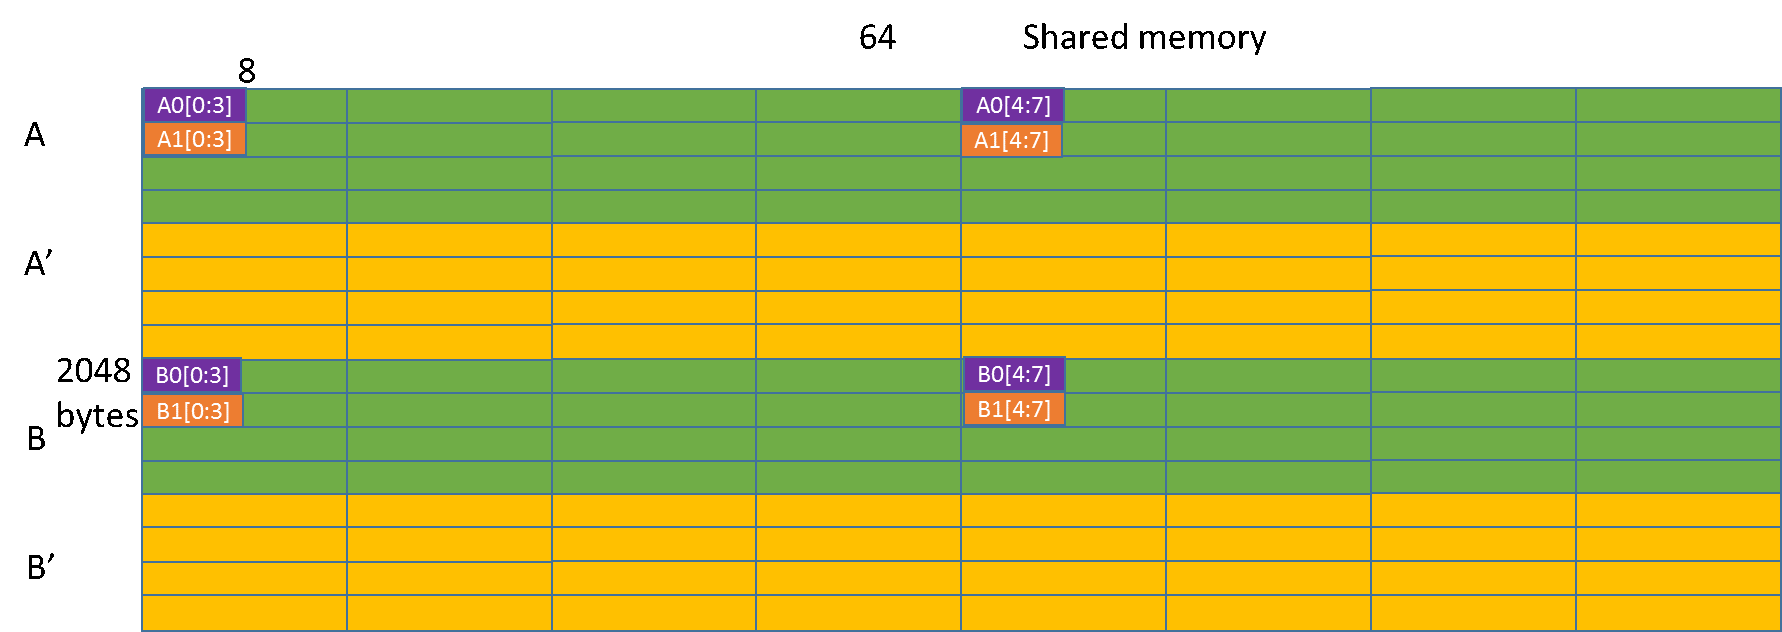
\includegraphics[width=0.50\textwidth]{readS}
	\bicaption{从共享内存读取A,B数据到寄存器}{Read A,B from shared memory to registers}
	\label{fig:readS}
\end{figure}

接下来就可以计算矩阵C了。图\ref{fig:readS}中紫色和橙色表示0号线程从局部共享内存要读取的数据。由于前面讲到了循环展开8次,紫色表示偶数次要读取的数据,橙色表示奇数次读取的数据绿色表示数据已经在共享内存中了,可以直接读取,黄色表示双缓冲的另外一半。

\begin{figure}[htbp]
	\centering
	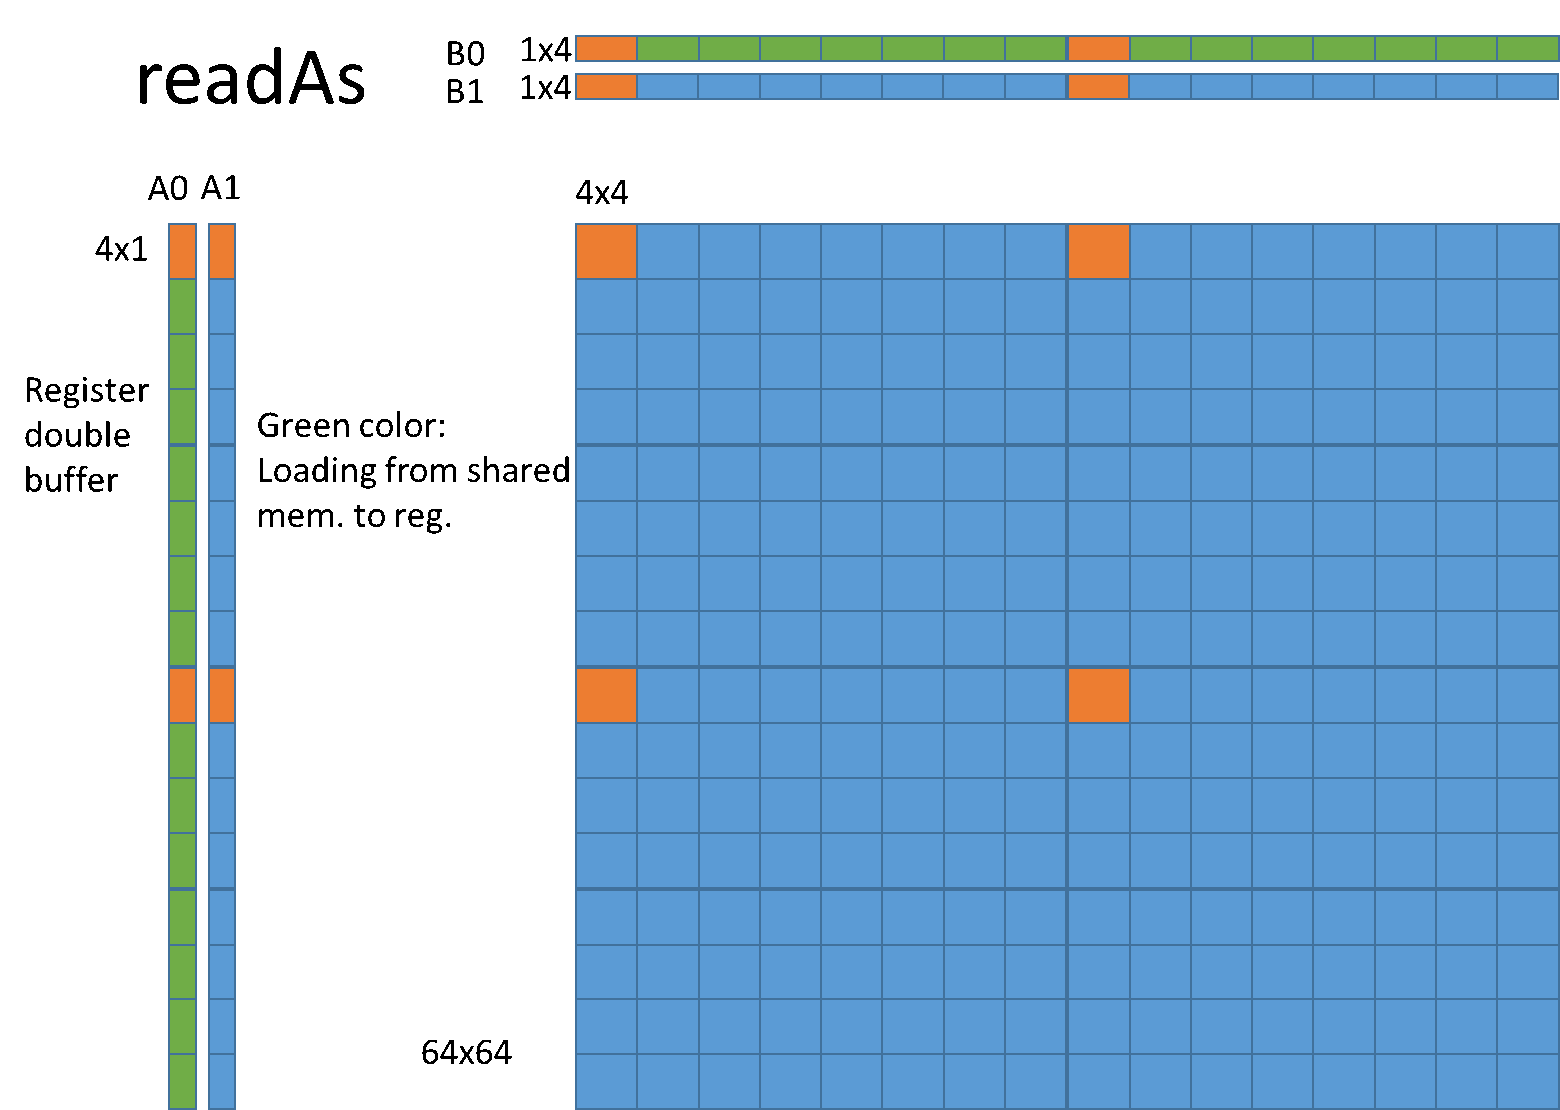
\includegraphics[width=0.50\textwidth]{threadblock}
	\bicaption{一个threadblock中的计算任务}{Computation tasks in a threadblock}
	\label{fig:threadblock}
\end{figure}

从block的角度观察每个线程的计算任务(如图\ref{fig:threadblock})。现在从一个block的角度来观察每个线程计算C的方式,这里一个block由一个wavefront组成,即64个线程, 一个block总共计算64x64个C中元素。图中橙色部分表示0号线程的计算任务,0号线程计算8x8的C,为了线程的负载均衡,这里将8x8分成4个4x4。这里总结一下:我们用了到数据预取,寄存器双缓冲,局部共享内存双缓冲,bank冲突消除,负载均衡,这些优化方法。


\section{将C矩阵从寄存器写回数据到全局内存}
当循环k/64次,每个线程块就可以把每个小块计算完成。此时需要把C存回全局内存。由于寄存器是私有的,每个线程只能存储自己计算的结果到对应的内存。可以做的优化是把C先从寄存器存回到共享内存,此时线程可以访问同一个线程块内的其他线程的计算结果。然后再从共享内存存储到全局访存。由于此时共享内存中的矩阵A和B的值以后将不再使用,所以不用开辟新的空间,直接复用A,B的空间即可。
通过乘加运算得到最终的结果C矩阵后,一般有两种方式将结果写回全局内存。第一种是先将C矩阵从寄存器写回到共性内存,然后再写回到全局内存;第二种是直接将C矩阵从寄存器写回到全局内存。
首先做4个v\_mul操作,将结果乘以系数alpha。然后用指令tbuffer\_store\_format\_xyzw依次写回4个结果。一个block总共需要写回64个元素,每4条v\_mul指令之间插入一条tbuffer\_store\_format\_xyzw指令。所有block并发执行,将整个C矩阵写回到全局内存。


\section{本章小结}
本章主要讲述了矩阵乘GPU实现的算法和具体实现步骤。描述了矩阵乘外积法的执行过程,并对比分析了外积法相比于內积法的优势。通过三个步骤讲述了外积法矩阵乘算法的数据的搬运和计算的执行过程。线程的映射关系,需要考虑全局访存能否联合访存,共享内存是否有bank冲突,如果遇到非分块整数倍的情况,任务能否均衡。根据本章提供的信息,读者可以复现本文的工作。
\chapter{矩阵乘优化与性能评估}\label{chap:GEMMOpt}

\section{实验配置}

本文实验的测试环境包括AMD Fiji服务器和AMD Vega服务器,其中每个服务器都是单节点,所用ROCm平台和操作系统版本相同。每个计算节点的软硬件主要参数如表\ref{tab:hardwareplatform}所示。
\begin{table}[htbp]
	\bicaption{实验平台软硬件主要参数}{Experimental platform hardware main parameters}
	\label{tab:hardwareplatform}
	\begin{center}
		\begin{tabular}{ | l | p{6cm} | p{6cm} |}
			\hline
			服务器 & AMD Fiji服务器 & AMD Vega服务器 \\ \hline
			GPU & Fiji R9 Nano & 2 x Vega10 \\ \hline
			%CPU & Intel(R) Xeon(R) CPU E5-2680 v3 @ 2.50GHz & 2 AMD EPYC 7451 24-Core Processor \\ \hline
			内存 & 251GB DDRM & 251GB DDRM \\ \hline
			操作系统 & Ubuntu16.04 & Ubuntu16.04 \\ \hline
			操作系统内核 & rocm-1.7 & rocm-1.7 \\ \hline
			OpenCL C version & OpenCL C 2.0 & OpenCL C 2.0 \\ \hline
			PCIe version & PCIe Gen3 & PCIe Gen3 \\
			\hline
		\end{tabular}
	\end{center}	
\end{table}


\section{矩阵乘性能调优}

\subsection{寄存器分块对v\_mac指令占比的影响}
\begin{figure}[htbp]
	\centering
	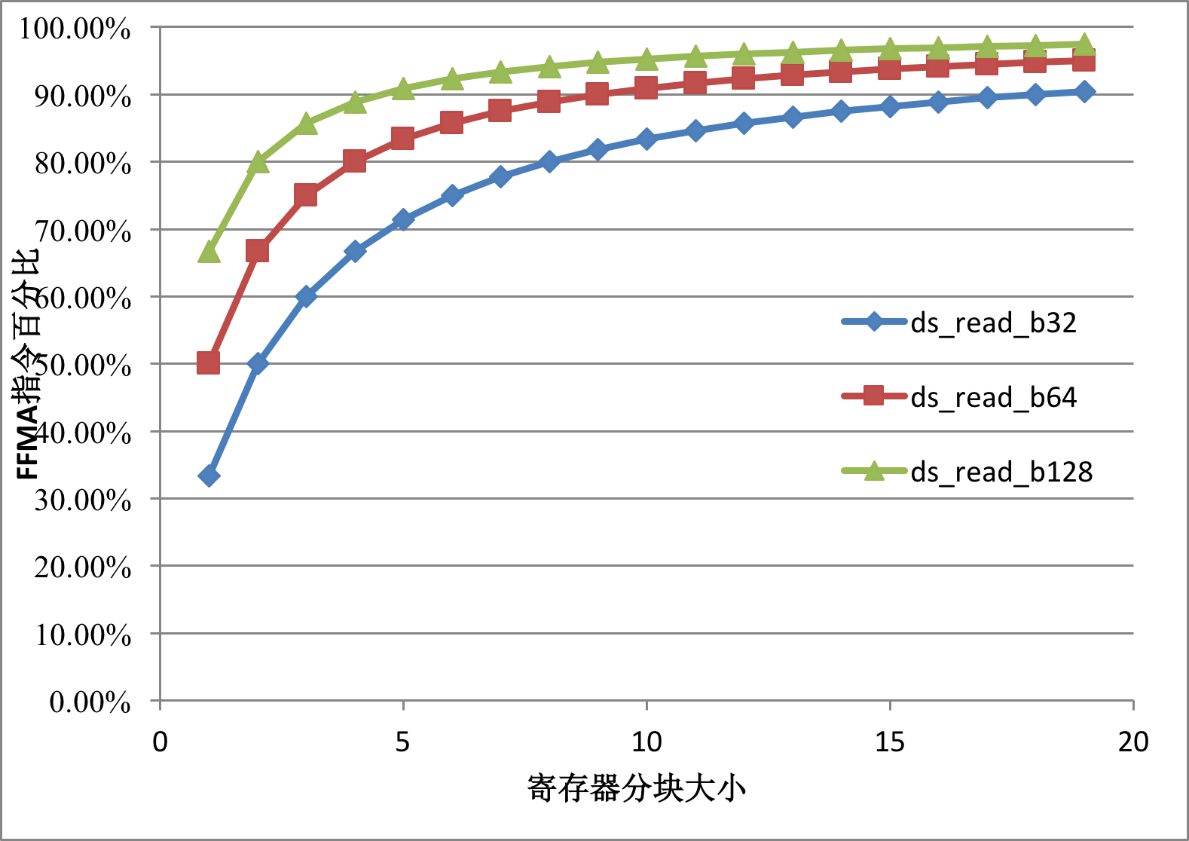
\includegraphics[width=0.60\textwidth]{ffma_percentage}
	\bicaption{v\_mac指令百分比随着寄存器分块大小的变化趋势}{The percentage of v\_mac instruction changes with the size of the register block}
	\label{fig:ffma_percentage}
\end{figure}

从图\ref{fig:ffma_percentage}中可以看出,随着寄存器分块大小增大,v\_mac指令百分比在提高。在寄存器分块大小不变的情况下,ds\_read\_bxx指令的位数宽度越宽,v\_mac指令百分比越高。如果采用的寄存器分块大小为6,则FFMA/DS\_READ\_B32=4:1,FFMA/DS\_READ\_B64=8:1,FFMA/DS\_READ\_B128=16:1。FFMA指令的百分比分别为80\%,88.89\%和94.12\%。

增大寄存器分块可以提高v\_mac指令的百分比,在v\_mac和ds\_read混合指令通量不变的情况下,v\_mac指令的百分比越高,v\_mac指令的通量越高。

\subsubsection{使用更宽的数据读指令}
为了实现更好的性能,在编写矩阵乘程序时,十分有必要将辅助指令的占比减到最小。这里的辅助指令是指非计算指令,尤其是指ds\_read指令。AMD GPU汇编提供了ds\_read\_b32,ds\_read\_b64和ds\_read\_b128指令,分别可从shared memory一次读32bit,64bit和128bit数据。使用更宽的读数据(load)指令可以减少ds\_read指令的数量。

对于AMD Fiji和Vega GPU,每个CU每一个shader cycle的ds\_read指令通量的峰值为32个32-bit。AMD GPU每个CU上每个SIMD有16个LD/ST单元,使用ds\_read\_b64就可以满足通量峰值,所以使用ds\_read\_b128指令不会增加读数据的通量。此时,在ds\_read\_b64和ds\_read\_b128和v\_mac混合指令通量相同的情况下,最好的情况是合理使用ds\_read\_b128指令,使用ds\_read\_b64的通量峰值将是ds\_read\_b32通量峰值的2倍。


\subsection{workgroup大小对访存带宽的影响}
根据workgroup的大小可以计算出所需的全局访存量,一个workgroup的计算任务为$b_m \times b_n$,$A$矩阵的维度为$M \times K$,$B$矩阵的维度为$K \times N$,由此可以计算出全局访存量为
\begin{equation}
\label{eq:globalmem}
\frac{M}{b_m} \times \frac{N}{b_n} \times K \times (b_m + b_n) = M \times N \times K \times (\frac{1}{b_m} + \frac{1}{b_n})
\end{equation}

由公式\ref{eq:globalmem}可知一个workgroup的计算量越多,全局访存量越少,但随着一个workgroup计算量的增多,其所需的局部共享内存也会增多,由于局部共享内存是一个CU上的有限资源,因此一个CU上并发的workgroup数会减少。对GPU而言CU上并发的workgroup数越多,越能隐藏高访存延迟。综上所述,workgroup大小会同时影响全局访存量和访存延迟隐藏。

\begin{table}[htbp]
	\bicaption{一个线程的数据搬移方向和搬移量}{Data movement direction and volume of a thread}
	\label{tab:thread_data_move}
	\begin{center}
		\begin{tabular}{ | l | l | }
			\hline
			Data path & Volume  \\ \hline
			global $\Rightarrow$ register & $\frac{r_x \times r_y}{b_n} \times b_k + \frac{r_x \times r_y}{b_m} \times b_k$  \\ \hline
			register $\Rightarrow$ shared & $\frac{r_x \times r_y}{b_n} \times b_k + \frac{r_x \times r_y}{b_m} \times b_k$  \\ \hline
			shared $\Rightarrow$ register & $r_x \times b_k + r_y \times b_k$ \\
			\hline
		\end{tabular}
	\end{center}	
\end{table}
在最内层循环中,每个线程共$2 \times r_x \times r_y$个浮点操作。表\ref{tab:thread_data_move}列出了主循环过程中一个线程的数据搬移方向和搬移量,包括全局内存到寄存器、寄存器到局部共享内存和局部共享内存再到寄存器。这样做的目的是充分挖局部共享内存和寄存器的数据重用。我们定义局部共享内存的计算密集度(Load data share arithmetic intensity)为浮点操作次数与局部共享内存访存次数的比例,其公式可表达如下\ref{eq:shared_arith_intensity}
\begin{equation}
\label{eq:shared_arith_intensity}
ldsAI = \frac{2 \times r_x \times r_y \times b_k}{r_x \times b_k + r_y \times b_k} = \frac{2}{\frac{1}{r_x} + \frac{1}{r_y}}
\end{equation}

每个线程需要$r_x$、$r_y$和$r_x \times r_y$分别存储A矩阵的一子列、B矩阵的一子行和C子矩阵。为了隐藏局部共享内存的访存延迟,我们使用了寄存器双缓冲。因此需要额外的$r_x$和$r_y$来预取下一次循环的A和B。由于所有寄存器总数不超过256的限制,我们可以得到公式\ref{eq:register_limit}
\begin{equation}
\label{eq:register_limit}
2 \times r_x + 2 \times r_y + r_x \times r_y < 256
\end{equation}
从公式\ref{eq:shared_arith_intensity}可知,寄存器分块越大局部共享内存计算密集度越高,在公式\ref{eq:register_limit}的限制条件下,当$r_x = r_y$时公式\ref{eq:shared_arith_intensity}取到最优值。因此寄存器分块可以选择$4\times 4$、$6\times 6$、$8\times8$、$12\times 12$等。
\section{汇编层次调优}
实际的SGEMM性能不会超过预估的SGEMM性能上界。对性能上界的评估比较理想化,因为这里主要考虑了影响性能的几个主要因素。除了前面考虑到的几个因素,也有其他因素可能会影响性能。实际的性能上界将介于预估性能上界和实际SGEMM性能之间。

根据A,B矩阵是否转置,可将SGEMM kernel可分4种情况,NN,NT,TN,TT(N表示不转置,T表示转置)。这里的分析中,主要考虑了两种类型的指令v\_mac和ds\_read\_bxx。在SGEMM中,还有其他的“辅助”指令对GFLOPS并没有贡献。“辅助”指令包括全局内存地址计算指令,shared memory地址计算指令等。同时,也没有考虑barrier指令对性能的影响。但实际上任何barrier指令都会降低程序性能。

\subsection{汇编调优的必要性}
使用高级语言(如OpenCL,CUDA)编写GPU程序的好处是开发速度快、易维护,但其对指令的控制能力相对较弱,同时程序编制人员对编译器的具体行为无法预测。有时编程人员对OpenCL或CUDA kernel所进行的手工优化可能会被编译器忽略掉,所以有时候编程人员编写的GPU程序性能会取决于编译器是否友好。

通过编写汇编kernel,编程人员可以直接跳过编译器,面向GPU硬件指令编程。这使得编程人员有机会进行更细粒度的程序调优。可以通过数据预取、寄存器双缓冲、shared memory双缓冲、bank冲突消除、指令重排等手法进行矩阵乘调优。其中OpenCL和汇编都可以使用数据预取,寄存器双缓冲和shared memory双缓冲和bank冲突消除这些手法进行程序优化。但只有通过汇编,程序编制人员才能进行细粒度的指令重排。在大量乘加指令之间的合适位置插入访存指令,尽可能用计算掩盖访存延迟,使得矩阵乘主循环中v\_mac指令通量接近v\_mac通量上界。

图\ref{fig:opencl_gemm_1_1_replot}展示了OpenCL实现的矩阵乘不同优化方法的性能比较。

\begin{figure}[htbp]
	\centering
	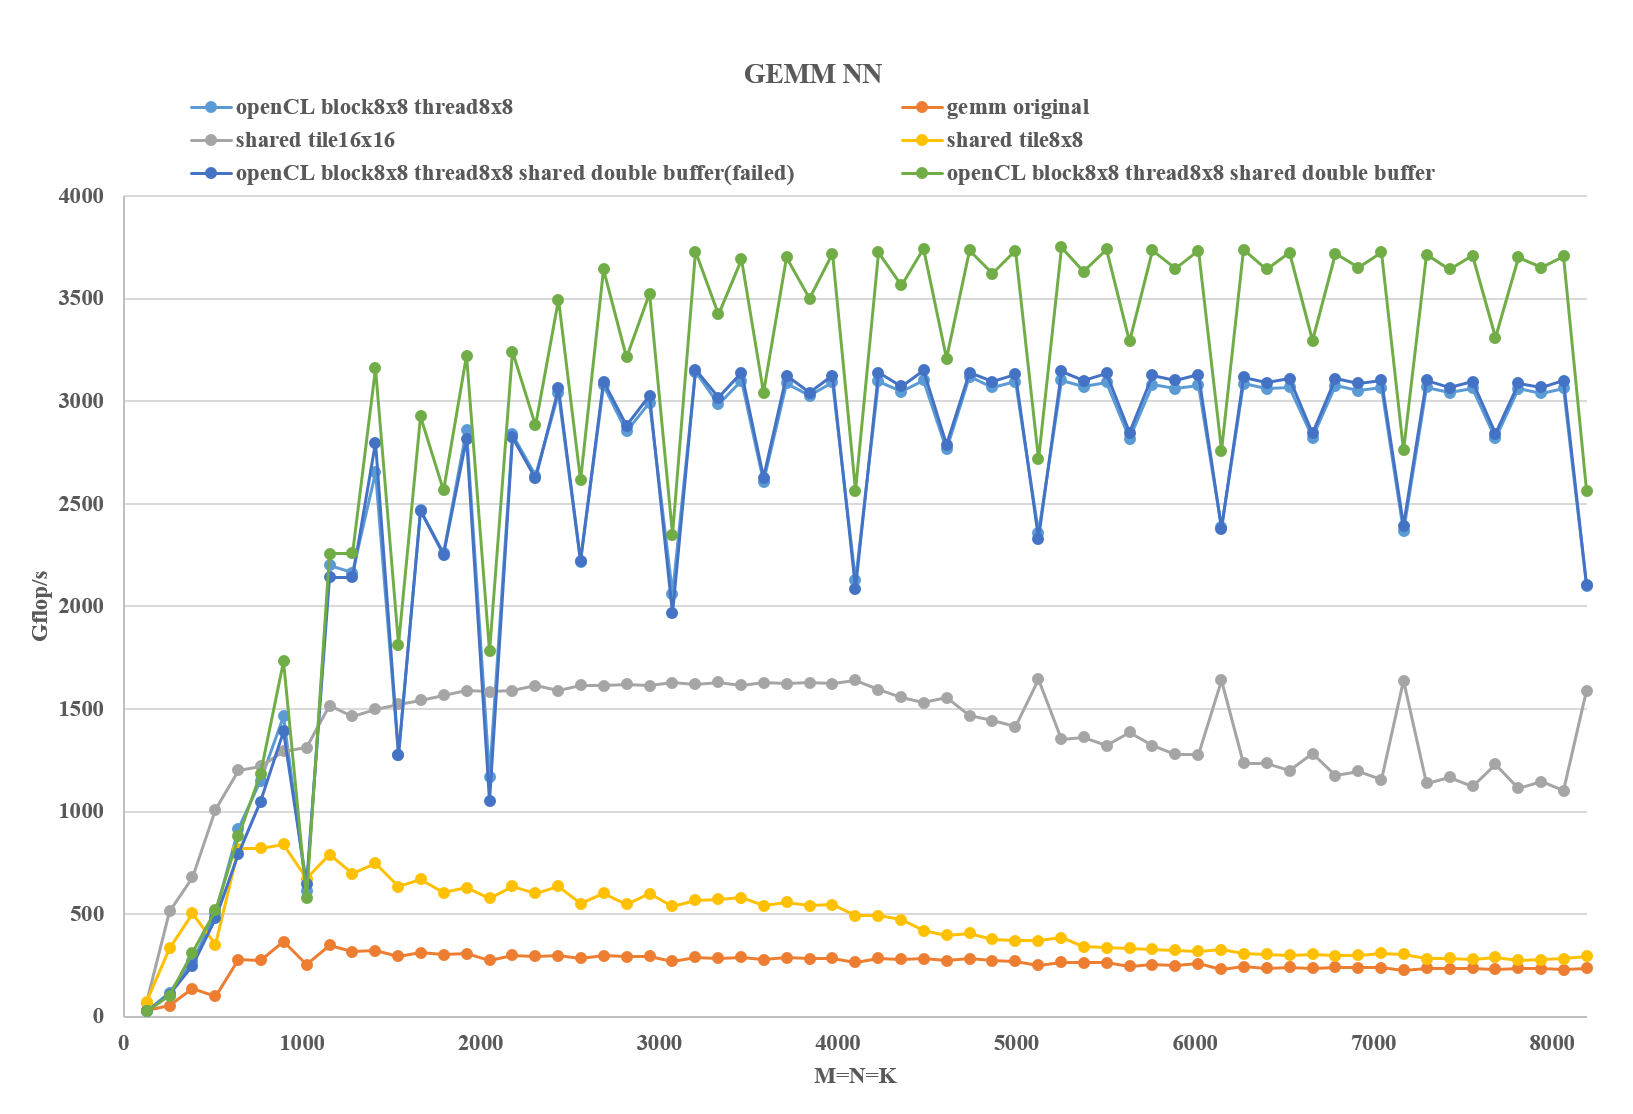
\includegraphics[width=0.80\textwidth]{opencl_gemm_1_1_replot}
	\bicaption{矩阵乘OpenCL实现性能比较}{Comparison of GEMM performance implemented by OpenCL}
	\label{fig:opencl_gemm_1_1_replot}
\end{figure}

从图\ref{fig:opencl_gemm_1_1_replot}可以看出,最简单的矩阵乘GPU实现其浮点效率最低(图\ref{fig:opencl_gemm_1_1_replot}中的gemm original曲线)。gemm original的实现没有使用shared memory,采用內积法每个线程计算一个输出。中间两条曲线表示使用shared memory,分块大小分别为8x8和16x16。由于矩阵乘在计算过程中有很多数据重用,利用数据重用的特点,将要计算的数据预先读入shared memory。在真正计算时从shared memory中取数据,可以减小数据读延迟。图\ref{fig:gemm_inner_product_tile}展示了使用shared memory分块的內积法矩阵乘。可以看出,计算C矩阵分块的同一行时,需要重复读A矩阵分块的同一行4个元素;同理,计算C矩阵分块的同一列时,要重复读B矩阵分块的同一列4个元素。全局内存读的次数减少4倍。分块大小为8时,全局内存读次数将减少8倍。所以在内存带宽受限时,提高shared memory分块大小可以减少全局内存读,降低内存带宽压力,提高计算性能。从图\ref{fig:opencl_gemm_1_1_replot}中可以看出16x16分块的性能高于8x8分块。

图\ref{fig:opencl_gemm_1_1_replot}中曲线openCL block8x8 thread8x8是原始的外积法矩阵乘实现。该矩阵乘的参数配置是,一个threadblock的线程数为8x8=64,在AMD GPU上即一个wavefront的大小。每个线程计算8x8的分块,因此一个threadblock计算64x64的输出。循环展开次数为8。写回结果时,直接从寄存器写回到全局内存。可见,外积法的矩阵乘性能从整体上要优于內积法。这是由于采用內积法可以并行地计算所有的乘法,但不能并行的计算加法。即使可以使用reduction来快速计算加法,但仍然会产生很多空闲的线程。这样,由于任务划分的不均衡,会使得计算性能大大降低。然而,如果用外积法来代替內积法,将会很大程度上缓解负载不均衡带来的性能损失。曲线openCL block8x8 thread8x8 shared double buffer表示在原始外积法实现的基础上进行了shared memory双缓冲的优化,性能得到进一步的提升。

\begin{figure}[htbp]
	\centering
	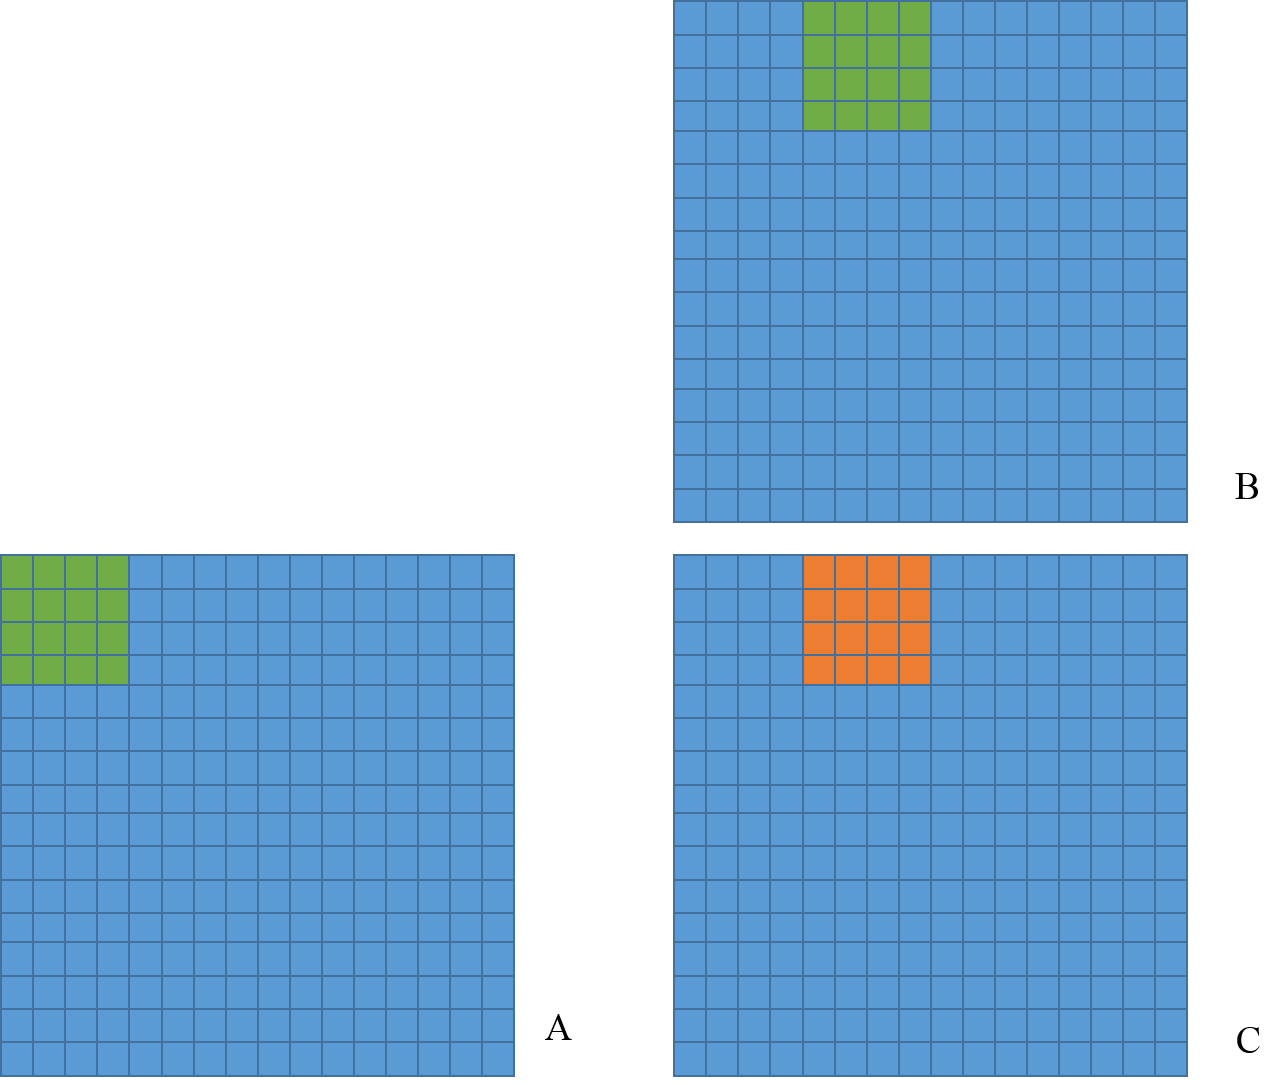
\includegraphics[width=0.60\textwidth]{gemm_inner_product_tile}
	\bicaption{內积法矩阵乘shared memory分块图示说明}{Illustration of inner-product GEMM with shared memory block}
	\label{fig:gemm_inner_product_tile}
\end{figure}

接下来进行外积法矩阵乘的shared memory bank冲突分析。图\ref{fig:shared_memory_bank_dist}展示了shared memory bank的分布情况。这里首先介绍一下AMD GPU shared memory的bank设计,shared memory有32的bank,每个bank的宽度为4字节。图\ref{fig:shared_memory_bank_dist}中绿色部分表示bank编号,蓝色部分表示一个block中A矩阵在shared memory中的分布情况,蓝色部分的同一列位于相同的bank。图中用其他颜色标注的部分,表示每个线程要读取的数据,例如(0,xxx)表示tid.x == 0,tid.y为0$\sim$7的线程要读取的8个元素。可以看出(0,xxx)线程和(4,xxx)线程都要读取bank0$\sim$bank7中的元素。图\ref{fig:bank0}展示了所有线程读bank0的情况。可以看出bank0的读取有4-way bank冲突。其他bank可类似分析。可以得知对于所有的bank,此时的shared memory有4-way bank冲突。

%bank冲突消除:


\begin{figure}[htbp]
	\centering
	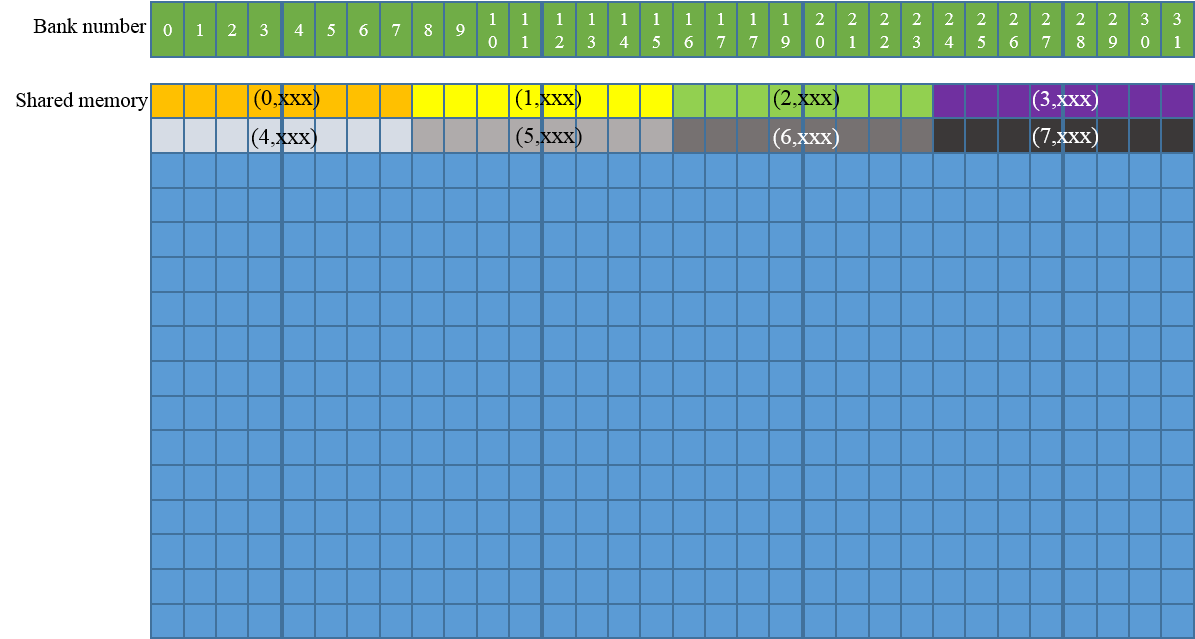
\includegraphics[width=0.80\textwidth]{shared_memory_bank_dist}
	\bicaption{shared memory bank分布}{Distribution of shared memory bank}
	\label{fig:shared_memory_bank_dist}
\end{figure}

\begin{figure}[htbp]
	\centering
	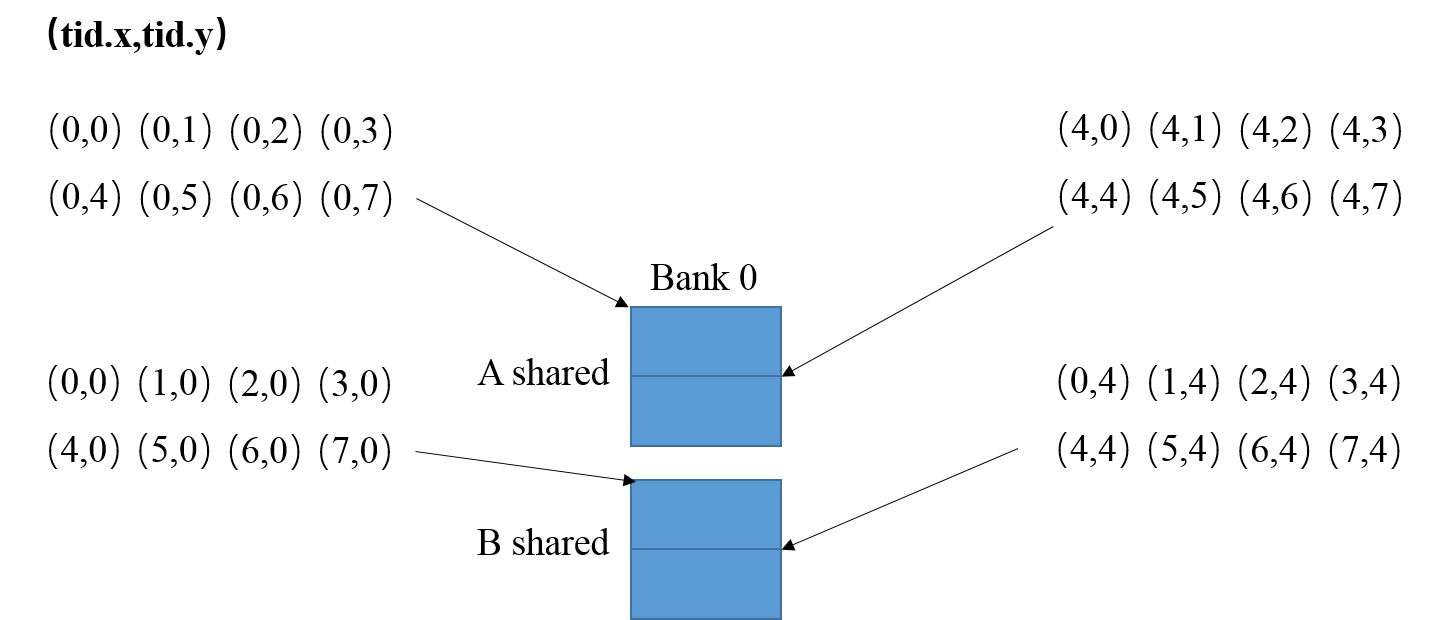
\includegraphics[width=0.80\textwidth]{bank0}
	\bicaption{4-way shared memory bank冲突}{4-way shared memory bank conflict}
	\label{fig:bank0}
\end{figure}

\subsection{优化内存访问}
汇编语言的访存优化和用高级语言(如CUDA,OpenCL)优化访存比较类似。一个wavefront(warp)中线程的全局访存请求可以合并成一到多个内存事务(memory transactions)。合并的方式和具体的GPU访存模式有关。为了高效的访问全局内存,通常我们安排一个wavefront中的线程访问全局内存中一段连续内存区域的数据。这样容易进行全局访存合并。在SGEMM程序的主循环中,主要的指令为v\_mac和ds\_read,为了提高v\_mac指令的百分比,减少ds\_read指令的数目就变得尤为关键。在前面的介绍中,讲到了可以通过使用DS\_READ\_B64或DS\_READ\_B128来减少DS\_READ指令数量。在shared memory中,线程读取A,B子矩阵也应该可以进行访存合并,我们安排每个线程可以读取连续的A,B子矩阵,一个wavefront中的线程可合并访问shared memory。同时,为了减少甚至消除shared memory的bank冲突和满足DS\_READ指令对齐的要求,在必要的时候,编程人员需要在shared memory中合理的进行填充。

\begin{figure}[htbp]
	\centering
	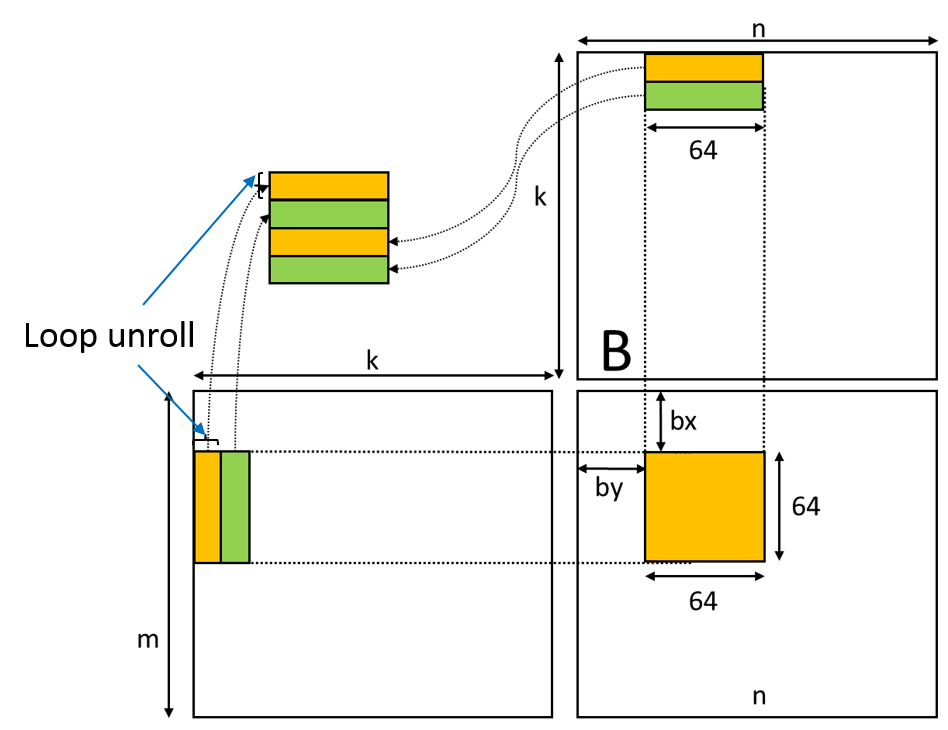
\includegraphics[width=0.50\textwidth]{loop_unroll_replot}
	\bicaption{循环展开图示}{Loop unroll}
	\label{fig:loop_unroll_replot}
\end{figure}
\subsection{循环展开}
通过循环展开(如图\ref{fig:loop_unroll_replot}),可以提高指令的通量。如下图中所示,沿着K方向做循环展开,这样在每次循环产生更多的浮点乘加操作,充分利用GPU上每个线程可拥有的寄存器个数。并且以循环展开作为前提,可以做后续的寄存器双缓冲,局部共享内存双缓冲等优化。通常都是做偶数次展开,这是为后面双缓冲要恰好是2的倍数做准备。在这里循环展开8次,考虑的因素有寄存器个数的限制,和局部共享内存容量的限制。循环展开的好处是能够减少很多冗余指令,减少分支判断指令的数目。对于GPU而言,执行分支判断指令只要用到标量部件就可以了,这极大浪费了GPU的向量计算单元,致使程序性能降低。

图\ref{fig:gemm_manual_unroll}展示了手工进行循环展开带来的性能提升。为了尽量避免OpenCL编译器的未知行为,编程人员可以进行手工循环展开。对于GPU而言,执行分支指令时大量的运算部件就处于空闲状态,这极大浪费了GPU大量的计算部件。手工循环展开的一个好处是可以减少分支指令的执行次数,给编程人员留出更多的优化空间。
\begin{figure}[htbp]
	\centering
	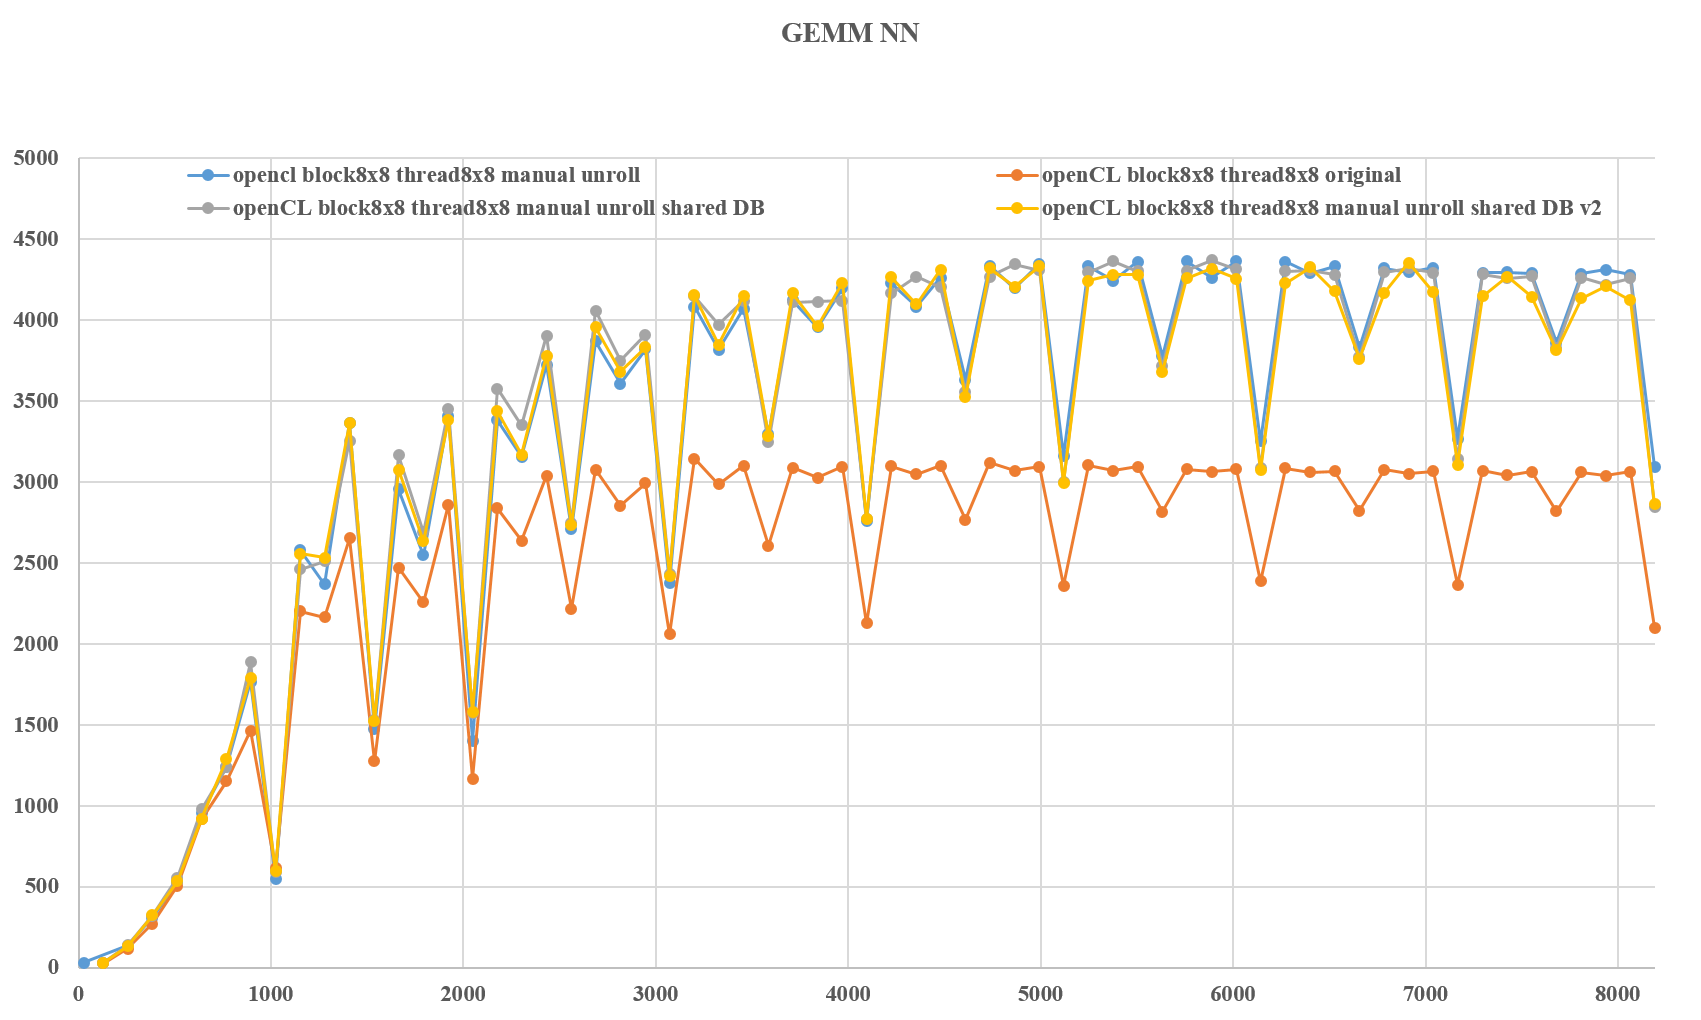
\includegraphics[width=0.80\textwidth]{gemm_manual_unroll}
	\bicaption{手工循环展开带来的性能提升}{Manual loop unroll}
	\label{fig:gemm_manual_unroll}
\end{figure}
\subsection{数据预取}
通过数据的预取可以减小计算时读取数据产生的等待延迟。从全局内存预取数据到共享内存,以增加一倍局部共享内存的代价来掩盖全局内存的访存延迟;从局部共享内存预取数据到寄存器,以增加一倍寄存器的代价来掩盖局部共享内存访存的延迟。

\subsection{shared memory双缓冲}
在前面的矩阵乘GPU算法描述中,讲述了shared memory的使用方法。首先将数据从全局内存读入寄存器,然后从寄存器写回到shared memory,最后再从shared memory读取数据到寄存器,并在寄存器中做计算。

为了更有效地利用shared memory,这里采用shared memory双缓冲。如算法\ref{alg:gemm_sharedmem_v1}所示,首先从全局内存预取数据到寄存器,然后从寄存器写回到shared memory。在从shared memory读取数据到寄存器并做计算之前,从全局内存预取下一次要计算的数据到寄存器。在OpenCL的实现中,shared memory双缓冲带来了$\sim$7.8\%的性能提升(如图\ref{fig:gemm_shared_double_buffer_replot})。
\begin{figure}[htbp]
	\centering
	\includegraphics[width=0.80\textwidth]{gemm_shared_double_buffer_replot}
	\bicaption{shared memory双缓冲带来的性能提升}{Shared memory double buffering brings performance improvements}
	\label{fig:gemm_shared_double_buffer_replot}
\end{figure}

\begin{algorithm}[htbp]
	\small
	\caption{GEMM algorithm with shared memory double buffer variant1}\label{alg:gemm_sharedmem_v1}
	\begin{algorithmic}[1]
		%\Procedure{Euclid}{$a,b$}\Comment{The g.c.d. of a and b}
		\State $A, B, C$\Comment{matrix A, B, C}
		\State $regA[task\_size],regB[task\_size],regC[task\_size]$\Comment{Allocate register for compute}
		\State $tileA[tile\_length*NUM\_UNROLL],tileB[tile\_length*NUM\_UNROLL]$\Comment{Shared memory double buffer}
		\State $tileA'[tile\_length*NUM\_UNROLL],tileB'[tile\_length*NUM\_UNROLL]$
		\State $loadA[tile\_length*NUM\_UNROLL/threadblock]$\Comment{Register for global memory load}
		\State $loadB[tile\_length*NUM\_UNROLL/threadblock]$
		\State $regC \gets 0$
		\State $loadA \gets A, loadB \gets B $\Comment{Pre load tile of A, B from global to register}
		\State barrier CLK\_GLOBAL\_MEM\_FENCE
		\For   {$i = 0$; $i < K/NUM\_UNROLL$; $++i$}
			\If    {$i \% 2 == 0$}
				\State $tileA \gets loadA, tileB \gets loadB$
				\State barrier CLK\_LOCAL\_MEM\_FENCE
				\State $loadA \gets A, loadB \gets B $\Comment{Load the next tile of A, B from global to register}
				\State barrier CLK\_GLOBAL\_MEM\_FENCE
					\For   {$k = 0$; $k<NUM\_UNROLL$;$++k$}\Comment{Loop Unroll}
						\State $regA \gets tileA, regB \gets tileB$
						\State $regC \gets regA \cdot regB + regC$
					\EndFor
			\Else  
				\State $tileA' \gets loadA, tileB' \gets loadB$
				\State barrier CLK\_LOCAL\_MEM\_FENCE
				\State $loadA \gets A, loadB \gets B $\Comment{Load the next tile of A, B from global to register}
				\State barrier CLK\_GLOBAL\_MEM\_FENCE
					\For   {$k = 0$; $k<NUM\_UNROLL$;$++k$}\Comment{Loop Unroll}
						\State $regA \gets tileA', regB \gets tileB'$
						\State $regC \gets regA \cdot regB + regC$
					\EndFor
			\EndIf
		\EndFor\label{gemmendfor}
		\State $C \gets regC$\Comment{Store C from registers to global memory}
		%\EndProcedure
	\end{algorithmic}
\end{algorithm}
两种shared memory双缓冲实现方式的的比较,第一种算法\ref{alg:gemm_sharedmem_v1}实现中,barrier CLK\_GLOBAL\_MEM\_FENCE语句放在全局内存读语句之后;第二种算法\ref{alg:gemm_sharedmem_v2}实现中,barrier CLK\_GLOBAL\_MEM\_FENCE语句放在寄存器写入数据到shared memory之前。从直观理解上第二种算法\ref{alg:gemm_sharedmem_v2}的性能应该优于第二种,因为第二种实现中将给全局内存到寄存器的数据读操作的延迟留出了更多的等待时间。但在AMD ROCm平台上实测的结果是第一种实现要好于第二种(图\ref{fig:gemm_shared_double_buffer_v2_replot}),第三种算法\ref{alg:gemm_sharedmem_v3}的整体性能要好于前两种算法,这里没有了if-else分支判断,产生了微弱的性能优势。从这里可以看出,编程人员有时对GPU编译器的行为无法做出预测,影响了更为细致的调优工作的开展。
\begin{figure}[htbp]
	\centering
	\includegraphics[width=0.80\textwidth]{gemm_shared_double_buffer_v2_replot}
	\bicaption{两种shared memory双缓冲实现的性能比较}{Performance comparison of two shared memory double buffering implementations}
	\label{fig:gemm_shared_double_buffer_v2_replot}
\end{figure}

\begin{algorithm}[htbp]
	\small
	\caption{GEMM algorithm with shared memory double buffer variant2}\label{alg:gemm_sharedmem_v2}
	\begin{algorithmic}[1]
		%\Procedure{Euclid}{$a,b$}\Comment{The g.c.d. of a and b}
		\State $A, B, C$\Comment{matrix A, B, C}
		\State $regA[task\_size],regB[task\_size],regC[task\_size]$\Comment{Allocate register for compute}
		\State $tileA[tile\_length*NUM\_UNROLL],tileB[tile\_length*NUM\_UNROLL]$\Comment{Shared memory double buffer}
		\State $tileA'[tile\_length*NUM\_UNROLL],tileB'[tile\_length*NUM\_UNROLL]$
		\State $loadA[tile\_length*NUM\_UNROLL/threadblock]$\Comment{Register for global memory load}
		\State $loadB[tile\_length*NUM\_UNROLL/threadblock]$
		\State $regC \gets 0$
		\State $loadA \gets A, loadB \gets B $\Comment{Pre load tile of A, B from global to register}
		\For   {$i = 0$; $i < K/NUM\_UNROLL$; $++i$}
		\If    {$i \% 2 == 0$}
		\State barrier CLK\_GLOBAL\_MEM\_FENCE
		\State $tileA \gets loadA, tileB \gets loadB$
		\State barrier CLK\_LOCAL\_MEM\_FENCE
		\State $loadA \gets A, loadB \gets B $\Comment{Load the next tile of A, B from global to register}
		\For   {$k = 0$; $k<NUM\_UNROLL$;$++k$}\Comment{Loop Unroll}
		\State $regA \gets tileA, regB \gets tileB$
		\State $regC \gets regA \cdot regB + regC$
		\EndFor
		\Else
		\State barrier CLK\_GLOBAL\_MEM\_FENCE  
		\State $tileA' \gets loadA, tileB' \gets loadB$
		\State barrier CLK\_LOCAL\_MEM\_FENCE
		\State $loadA \gets A, loadB \gets B $\Comment{Load the next tile of A, B from global to register}
		\State barrier CLK\_GLOBAL\_MEM\_FENCE
		\For   {$k = 0$; $k<NUM\_UNROLL$;$++k$}\Comment{Loop Unroll}
		\State $regA \gets tileA', regB \gets tileB'$
		\State $regC \gets regA \cdot regB + regC$
		\EndFor
		\EndIf
		\EndFor\label{gemmendfor}
		\State $C \gets regC$\Comment{Store C from registers to global memory}
		%\EndProcedure
	\end{algorithmic}
\end{algorithm}

\subsection{寄存器双缓冲}
如图\ref{fig:reg_double_buffer_replot}所示,可以在用寄存器A1,B1计算的同时,从局部共享内存取下一次要计算的数据到寄存器A0,B0。由于数据的预取,在进入循环前,已经将第一次要计算的数据读到了寄存器A0[0:7],B0[0:7]中。

每个线程使用A1,B1寄存器中的数据,做本次的8x8乘加操作;在线程做本次乘加操作的同时,从局部共享内存预取下一次的数据到寄存器A0,B0。通过寄存器双缓冲,可以用计算掩盖从局部共享内存读的延迟。沿着K方向循环展开8次,分成0,2,4,6 和 1,3,5,7。一半奇数,一半偶数。偶数次时,每个线程从shared memory预取8个a到寄存器A1[0:7],8个b到寄存器B1[0:7], 即预取下一次(奇数时)计算需要的8个a和8个b。奇数次时,每个线程从shared memory预取8个a到寄存器A0[0:7],8个b到寄存器B0[0:7], 即预取下一次(偶数时)计算需要的8个a和8个b。偶数次循环计算A0[0:7]*B0[0:7],奇数次循环计算 A1[0:7]*B1[0:7]。对每个线程来说,需要计算8x8个输出,共需要做64次乘加操作。从共享内存读,一次读4个连续元素,读8个a和8个b,需要4个共享内存读指令。这样就可以用寄存器的计算,来掩盖共享内存读的延迟。

\begin{figure}[htbp]
	\centering
	\includegraphics[width=0.50\textwidth]{reg_double_buffer_replot}
	\bicaption{寄存器双缓冲}{Register double buffer}
	\label{fig:reg_double_buffer_replot}
\end{figure}

\begin{algorithm}[htbp]
	\small
	\caption{GEMM algorithm with shared memory double buffer variant3}\label{alg:gemm_sharedmem_v3}
	\begin{algorithmic}[1]
		%\Procedure{Euclid}{$a,b$}\Comment{The g.c.d. of a and b}
		\State $A, B, C$\Comment{matrix A, B, C}
		\State $regA[task\_size],regB[task\_size],regC[task\_size]$\Comment{Allocate register for compute}
		\State $tileA[tile\_length*NUM\_UNROLL],tileB[tile\_length*NUM\_UNROLL]$\Comment{Shared memory double buffer}
		\State $tileA'[tile\_length*NUM\_UNROLL],tileB'[tile\_length*NUM\_UNROLL]$
		\State $loadA[tile\_length*NUM\_UNROLL/threadblock]$\Comment{Register for global memory load}
		\State $loadB[tile\_length*NUM\_UNROLL/threadblock]$
		\State $regC \gets 0$
		\State $loadA \gets A, loadB \gets B $\Comment{Pre load tile of A, B from global to register}
			\For   {$i = 0$; $i < K/NUM\_UNROLL$; $++i$}
				\State barrier CLK\_GLOBAL\_MEM\_FENCE
				\State $tileA \gets loadA, tileB \gets loadB$
				\State barrier CLK\_LOCAL\_MEM\_FENCE
				\State $loadA \gets A, loadB \gets B $\Comment{Load the next tile of A, B from global to register}
					\For   {$k = 0$; $k<NUM\_UNROLL$;$++k$}\Comment{Loop Unroll}
						\State $regA \gets tileA, regB \gets tileB$
						\State $regC \gets regA \cdot regB + regC$
					\EndFor
				\State $tileA \leftrightarrow tileA', tileB \leftrightarrow tileB'$\Comment{Swap double buffer}
			\EndFor\label{gemmendfor}
		\State $C \gets regC$\Comment{Store C from registers to global memory}
		%\EndProcedure
	\end{algorithmic}
\end{algorithm}

\subsection{线程负载均衡}
对每个线程来说,使用4个4x4,来代替8x8的计算方式,来使得一个block中的线程可以负载均衡(如图\ref{fig:load_balance_replot})。在进行shared memory bank冲突消除时,同时做到了线程的负载均衡。将一个threadblock的计算任务均等的划分成4份。所有线程都分别计算4份中的每一个中相应的元素。例如,0号线程分别计算4个分块的左上角的4x4的输出。通过这种方式,可以提高一个block的计算效率。
\begin{figure}[htbp]
	\centering
	\includegraphics[width=0.50\textwidth]{load_balance_replot}
	\bicaption{线程负载均衡}{Thread load balance}
	\label{fig:load_balance_replot}
\end{figure}


\subsection{消除shared memory bank冲突}
AMD GPU shared memory有32个bank。当不同的线程访问不同的bank时,线程可以同时读;当不同的线程访问同一个bank的同一个位置时,可以进行广播;当不同的线程访问同一个bank的不同位置时,会产生bank冲突,需要多个时钟周期来完成。所以,bank冲突会减小访存带宽,对性能影响很大。

在前面的6.3.1小结中,分析了外积法的原始实现中,有4-way shared memory bank冲突。通过观察可以发现,产生shared memory bank冲突的原因是在一个threadblock中,所有线程对shared memory的访问跨越了2个bank,导致不同的线程访问同一个的bank的不同entry这种情况发生。接下来,将展示如何通过分配线程的计算任务来消除shared memory bank冲突。消除shared memory bank冲突的方法是安排一个thread block中的所有线程对shared memory的一次访问限制在一个bank中。图\ref{fig:gemm_no_bank_conflict_replot}展示了通过消除shared memory bank冲突所带来的性能提升。从图\ref{fig:gemm_no_bank_conflict_replot}看出,通过消除bank冲突可以带来微弱的性能提升,这里的一个原因是这里的shared memory bank冲突消除是在原始的外积法矩阵乘的基础上实现的。此时矩阵乘瓶颈还在全局访存。没有用到shared memory双缓冲,因此提升的性能不多。

\begin{figure}[htbp]
	\centering
	\includegraphics[width=0.80\textwidth]{gemm_no_bank_conflict_replot}
	\bicaption{shared memory bank冲突消除带来的性能提升}{Performance improvements with shared memory bank conflict elimination}
	\label{fig:gemm_no_bank_conflict_replot}
\end{figure}


图\ref{fig:gemm_shared_db_no_bank_conflict_replot}展示了在外积法原始实现版本中分别加入shared memory双缓冲和bank冲突消除优化手法所带来的性能提升。
\begin{figure}[htbp]
	\centering
	\includegraphics[width=0.80\textwidth]{gemm_shared_db_no_bank_conflict_replot}
	\bicaption{shared memory 双缓冲,无bank冲突的性能表现}{GEMM performance with shared memory DB and bank conflict elimination}
	\label{fig:gemm_shared_db_no_bank_conflict_replot}
\end{figure}
图\ref{fig:bank_conflict_replot}中小方格中的数字表示一个block中的64个线程,将64个线程看成一个2维的线程数组tid.x 取值为0$\sim$7, tid.y取值为0$\sim$7。小方格中的数字对(tid.x,tid.y)对应的线程号为tid = tid.y * 8 + tid.x。可以看到,图\ref{fig:bank_conflict_replot}中同一行的线程读4个连续的bank,没有bank冲突;不同线程读相同的位置,会在同一行进行广播;图中同一列的线程读4个连续的bank没有bank冲突会在同一列进行广播。因此通过设计这种共享内存读的方式可以完全消除bank冲突。
\begin{figure}[htbp]
	\centering
	\includegraphics[width=0.70\textwidth]{bank_conflict_replot}
	\bicaption{shared memory bank冲突消除}{Shared memory bank conflict elimination}
	\label{fig:bank_conflict_replot}
\end{figure}


\subsection{指令重排}
通常编程人员尝试将不同类型的指令交错放置来使得一个CU上不同的功能部件可以均衡的利用起来,进而获得更高的指令通量。本文采用下面的指令重排方法。将全局内存数据预取指令和v\_mac,DS\_READ指令交错放置来获得更高的性能。图\ref{fig:none_f_mac_inst}展示了矩阵乘主循环中非v\_mac指令的位置。
\begin{figure}[htbp]
	\centering
	\includegraphics[width=1.0\textwidth]{none_f_mac_inst}
	\bicaption{非v\_mac指令的位置}{None v\_mac inst slot}
	\label{fig:none_f_mac_inst}
\end{figure}

%	
%\begin{table}[!htbp]
%	\bicaption{非v\_mac指令的位置}{Instruction position of the none v\_mac}
%	\label{tab:thread_data_move}
%	%\centering
%	\begin{center}
%		 \resizebox{\textwidth}{18mm}{ 
%		\begin{tabular}{|l|l|l|l|l|l|l|l|l|}
%			\hline
%			\diagbox {slot}{unroll} & $0$ & $1$ & $2$ & $3$ & $4$ & $5$ & $6$ & $7$\\ %添加斜线表头
%			\hline
%			$0$ & 4x ds\_read\_b128 & 4x ds\_read\_b128 & 4x ds\_read\_b128 & 4x ds\_read\_b128 & 4x ds\_read\_b128 & 4x ds\_read\_b128 & 4x ds\_read\_b128 & 4x ds\_read\_b128 \\
%			\hline
%			\multirow{3}*{$24$} & t\_buffer\_load\_xyzw  &  & s\_waitcnt vmcnt(3)& & t\_buffer\_load\_xyzw & & s\_waitcnt vmcnt(3) & \\
%			~                   &                        &  & ds\_write\_b128    & &                       & & ds\_write\_b128     & \\
%			~                   &                        &  &                    & &                       & & s\_add\_u32         & \\
%			\hline
%			%$24$ & t\_buffer\_load\_xyzw  &  & s\_waitcnt vmcnt(2)  ds\_write\_b128 & & t\_buffer\_load\_xyzw v\_add\_u32 trackA v\_add\_u32 trackB & & s\_waitcnt vmcnt(3) ds\_write\_b128 s\_cmp\_gt\_u32 & %\\
%			\hline
%		\end{tabular}}
%	\end{center}
%\end{table}
%	
%%\end{document}


\subsubsection{指令重排的几个原则}
(1) 从shared memory中预取数据到寄存器的指令:尽可能地早放置。

ds\_read\_b128指令用于从shared memory中预取数据到寄存器。循环展开8次,每次计算8x8个输出。总共8x8x8 = 512条v\_mac指令。一条ds\_read\_b128指令可以从shared memory中取4个浮点元素。计算8x8的输出需要8个A中对应元素和8个B中对应元素,因此需要(8+8)/4 = 4 条ds\_read\_b128指令。在计算本次8x8个v\_mac时,要预取下一个8x8个v\_mac所需的指令。为了给ds\_read\_b128指令从发射到结果返回留出足够多的时间,放置ds\_read\_b128指令的原则是尽可能地早发射ds\_read\_b128指令,所以在每次8x8个v\_mac最开始的位置之前插入4条ds\_read\_b128指令。

(2) 从全局内存读取数据到寄存器:尽可能地早放置。

t\_buffer\_load\_xyzw指令用于从全局内存预取数据到寄存器。一个block有64个线程,每个线程计算8x8个输出,总共可以计算64x64个输出。t\_buffer\_load\_xyzw指令一次可以从全局内存读取4个元素,计算64x64的输出,循环展开8次,需要8x64个A中对应元素和8x64个B中对应元素。因此每个线程需要(8x64+8x64)/(4x64) = 4条t\_buffer\_load\_xyzw指令。(3) 从寄存器写入数据到shared memory:和全局内存读指令间隔足够远。

为了数据重用,把从全局内存读到寄存的数据写入shared memory。使用ds\_read\_b128指令将数据从存寄存器写入shared memory。ds\_read\_b128指令要等对应的t\_buffer\_load\_xyzw指令结果返回,所以ds\_read\_b128指令和t\_buffer\_load\_xyzw要间隔得足够远。

从图\ref{fig:none_f_mac_inst}可以观察出在每个8x8的循环的起始位置插入4条ds\_read\_b128指令,这4条指令是为下一个8x8循环进行预取。在第0次展开的24和32的位置插入两条全局内存读指令t\_buffer\_load\_xyzw,这两条指令也是在进行数据预取。为了让全局内存读指令和共享内存写指令间隔的尽可能地远,在第6次展开的24和32位置插入共享内存写指令ds\_write\_b128。其中最为巧妙的是利用s\_waitcnt vmcnt()指令来精确地等待某一条全局内存读指令的完成。第6次展开的24位置s\_waitcnt vmcnt(3)指令表示3条全局访存指令还未完成,即按顺序发射了4条访存指令,其中第1条访存指令结果已经返回,剩下3条指令结果还未返回,这样就是在等待第1条指令结果返回然后继续执行,否则就等待。其他指令的位置可类似分析。同时相比于OpenCL,手工编写汇编可以去除冗余指令,在OpenCL中只能使用barrier指令来进行等待,手工编写汇编可以去除barrier指令使用更为准确的s\_waitcnt指令进行等待。


\section{矩阵乘性能测试}
通过实际测试(如图\ref{fig:hgemm_perf}),矩阵乘性能峰值可达$\sim$95\%。图\ref{fig:gemm_tuning_comp}展示了分别采用循环展开,shared memory双缓冲,bank冲突消除,寄存器双缓冲和指令重排所带来的一步步性能提升。对比了AMD官方库rocBLAS和Tensile,相比roclBLAS,最高有$\sim$20\%的性能提升,对比自动调优库Tensile生成的汇编矩阵乘有略微的性能优势,最多有3\%$\sim$5\%的性能提升。
\begin{figure}[htbp]
	\centering
	\includegraphics[width=0.80\textwidth]{hgemm_perf}
	\bicaption{汇编调优的矩阵乘性能展示}{GEMM performance}
	\label{fig:hgemm_perf}
\end{figure}
\begin{figure}[htbp]
	\centering
	\includegraphics[width=0.80\textwidth]{gemm_tuning_comp}
	\bicaption{矩阵乘性能变化趋势}{GEMM performance tuning}
	\label{fig:gemm_tuning_comp}
\end{figure}
这里需要说明的是在本次测试中使用的矩阵规模都是正方形,即M=N=K的情况,并且都是64的整数倍,对非64整数倍的矩阵尺寸没有进行边界处理。矩阵数据采用随机函数进行生成。其中循环展开,shared memory双缓冲和寄存器双缓冲带来了大部分的性能能提升,这得益于利用shared memory和寄存器隐藏了全局内存读延迟。

指令细粒度重排只有用汇编才可实现,OpenCL可以使用的同步指令只有barrier CLK\_GLOBAL\_MEM\_FENCE和barrier CLK\_LOCAL\_MEM\_FENCE这两种;而在汇编语言中,通过使用s\_waitcnt vmcnt()可以具体等待某一条访存指令的完成,同时,也没有OpenCL编译器所带来的无法预测的行为。通过利用前面讲到的指令重排的几个原则,进一步掩盖访存延迟,获得计算性能的提升。


\section{矩阵乘性能分析}
\subsection{矩阵乘潜在性能峰值}
在寄存器分块大小为8x8,block线程数为64的情况下。v\_mac峰值性能为512/(512+24+2) = 512/538 = 95.17\%。这里在计算上认为32条ds\_read\_b128有只有8条指令双发射。实际处理器的执行行为需要通过测试可以得知。
\begin{table}[htbp]
	\bicaption{矩阵乘主循环指令构成}{GEMM main loop instructions}
	\label{tab:fijiFFMA}
	\begin{center}
		\begin{tabular}{ | l | p{4cm} |}
			\hline
			Operation & Count \\ \hline
			v\_mac & 512  \\ \hline
			ds\_read\_b128 & total 32, 8 dual issue \\ \hline
			ds\_write\_b128 & 4 dual issue \\ \hline
			tbuffer\_load\_xyzw & 4 dual issue \\ \hline
			v\_add\_u32 & 2 \\ \hline
			s\_waitcnt vmcnt() & 4 dual issue \\ \hline
			s\_add\_u32 & 1 dual issue \\ \hline
			s\_cmp\_gt\_u32 & 1 dual issue \\ \hline
			s\_cbranch\_scc0 & 1 daul issue \\
			\hline
		\end{tabular}
	\end{center}	
\end{table}

如果在执行时,将每4条ds\_read\_b128指令合并,则32条ds\_read\_b128全部都双发射。此时的v\_mac峰值性能为512/(512+2) = 99.61\%(如表\ref{tab:fijiFFMA})。

\subsection{Roofline模型}
Roofline\citepns{williams2009roofline}模型是Williams和Patterson等人在2008年提出的一个可视化应用程序性能分析模型,用于分析多核计算机系统上的浮点计算程序性能。该模型为并行软件和多核计算机体系结构的设计提供了有用的指导。Roofline模型从计算量和访存量这两个方面来描述浮点计算程序和多核计算机体系结构的性能。当浮点部件未充分使用时,随着内存带宽的提升浮点计算性能跟着提升,此时的程序性能瓶颈为内存带宽受限;当浮点部件被完全使用时,随着内存带宽的提升浮点计算性能不再变化,此时的程序性能瓶颈为计算受限。
\begin{equation}
\label{eq:global_arith_intensity}
gmemAI = \frac{2 \times b_m \times b_m \times b_k}{4\times (b_m \times b_k + b_n\times b_k)} = \frac{Gflops}{bandwidth}
\end{equation}

\begin{figure}[htbp]
	\centering
	\includegraphics[width=1.0\textwidth]{roofline_global}
	\bicaption{全局内存的roofline模型}{Global memory roofline model}
	\label{fig:roofline_global}
\end{figure}

图\ref{fig:roofline_global}展示了AMD Fiji GPU的全局内存Roofline模型,黑色实线代表机器理论峰值,横坐标为计算和全局内存访存比例,纵坐标为机器理论浮点峰值。在矩阵乘的主循环中,每个线程块计算量为$2\times b_m \times b_n \times b_k$次浮点操作,访存量为$4\times (b_m \times b_k + b_n\times b_k)$个字节,因此每个线程块的计算和全局内存访存比例(Global memory arithmetic intensity)可由公式\ref{eq:global_arith_intensity}计算得出。

在我们实现的矩阵乘算法中,$b_m = b_n = 64$,$b_k = 8$。AMD Fiji GPU的最高浮点性能为8192 Gflop/s,对全局内存带宽的最低要求是512 GB/s。Fiji GPU可以提供的全局访存带宽为$Global_{bandwidth} = 2 \times f_{mem} \times W = 2 \times 500MHz \times 4096bit = 512GB/s$,可以满足矩阵乘算法对全局访存带宽的要求。可以看到$4\times 4$寄存器分块算法的计算访存比为8,其对应的浮点性能峰值为4096 Gflop/s,此时矩阵乘的性能严重受到全局内存访存带宽的限制;$8\times 8$寄存器分块算法正好处在Roofline模型的拐点处,矩阵乘不受全局内存访存带宽的限制。寄存器分块越大,计算和全局内存访存比例越大,越接近机器理论峰值。


\section{本章小结}
本章首先介绍了本次实验所使用的计算环境,然后分析了寄存器分块的大小和读数据指令的位宽对浮点通量的影响,接下来详细描述了矩阵乘调优的过程。分别展示了循环展开、shared memory双缓冲、bank冲突消除、寄存器双缓冲和指令重排这些优化方法所带来的一步步性能提升,并和AMD官方数学库rocBLAS和Tensile的矩阵乘性能进行了对比。其中循环展开,shared memory双缓冲和寄存器双缓冲带来了大部分的性能能提升,这得益于利用shared memory和寄存器隐藏了全局内存读延迟。指令细粒度重排只有用汇编编写才能实现,因为在OpenCL层面,可以使用的同步指令只有barrier CLK\_GLOBAL\_MEM\_FENCE和barrier CLK\_LOCAL\_MEM\_FENCE这两种;而在汇编语言中,通过使用s\_waitcnt vmcnt()可以具体等待某一条访存指令的完成,同时,也没有OpenCL编译器所带来的无法预测的行为。通过利用前面讲到的指令重排的几个原则,进一步掩盖访存延迟,获得计算性能的提升。最后通过统计主循环中每种指令的个数和单双发射的情况,进行了矩阵乘性能上界分析。


\chapter{结束语}\label{chap:Conclusion}

\section{本文工作总结}
本文研究对AMD GPU矩阵乘算法进行并行加速。 

本文首先分析了AMD GPU架构细节,分析了当前主流GPU矩阵乘的优化工作。总结了NVIDIA GPU矩阵乘的优化手法,将该手法结合AMD Fiji和Vega架构,设计了Fiji和Vega架构矩阵乘,并进行了调优工作。实现了AMD GPU高效的矩阵乘。

在开始做AMD GPU矩阵乘调优时,使用了AMD Fiji和Vega GPU。首先通过AMD官网找到Fiji和Vega GPU架构的ISA手册,阅读与分析ISA手册,开始对AMD GPU的架构有所了解。接下来开始测AMD的rocBLAS,MIOpenGEMM和Tensile等数学库的矩阵乘性能,并分析其中的GEMM kernerl。一开始的研究计划是同时考虑做自动调优和手工调优。在现有的AMD GPU开源数学中,有官方的rocBLAS库,也有第三方开源库如CLBlast\citepns{nugteren2017clblast}。CLBlast目前维护的比较好,其整体性能要略好于rocBLAS,是一个很好的工作。AMD GPU现有GEMM自动调优库有MIOpenGEMM和Tensile。从性能上,Tensile要好于MIOpenGEMM,Tensile可以将矩阵乘的性能通过自动调优接近91\%。缺点是Tensile生成kernel的时间要比MIOpenGEMM长很多。MIOpenGEMM目前集成在MIOpen卷积数学库中。Tensile集成在rocBLAS中。我用了较多时间阅读MIOpenGEMM和Tensile库的源码,分析其中的技术要点和设计原理。手工优化GEMM的方法主要来源于Junjie Lai在Fermi和Kepler GPU上的GEMM调优工作和GEMM性能上界分析以及Scott Gray针对Maxwell架构做的maxas SGEMM的工作。

本文通过分析AMD GPU 微架构细节,采用寄存器分块、双缓冲、bank冲突消除、指令重排等手工汇编优化的方法,在 AMD Fiji 和 Vega GPU 上实现的矩阵乘效率达到95\%。本文分析了AMD GPU矩阵乘的性能上界,可以知道我们当前实现的矩阵乘效率距离矩阵乘性能上界还有多远。这种分析方法具有通用性,可以将这种方法稍加修改就可以应用于其他GPU应用程序性能上界的分析。为我们的调优工作提供了指导方向。

\section{下一步工作}
本文的工作是基于AMD GPU的通用矩阵乘调优。采用手工汇编优化的手法,通过寄存器分块,寄存器双缓冲,shared memory双缓冲等,指令调度等手法一步步提高矩阵乘性能。采用手工汇编优化的优点是可以通过十分细粒度的指令调度将矩阵乘的性能尽可能调高;同时也有缺点,一方面进行手工优化需要深入理解AMD GPU的架构细节,理解AMD GPU的内存层次结构,指令的调度方式,寄存器,shared memory等资源的大小,另一方面也要有丰富的程序优化经验,和汇编程序编制和调试的编程基础。同时,如果AMD GPU架构发生变化时,我们就要重复这种调优工作。另一种做AMD GPU矩阵乘的方向是自动调优,通过benchmark的方法自动找出较优的矩阵乘kernel。自动调优可以自动生成针对不同架构的矩阵乘kernel。免去了手工重复调优的工作。但一般来说,手工优化的kernel性能会高于自动调优工具。

自动调优会涉及到编译领域的相关技术。编写代码模板,代码自动生成等。自动调优可提高kernel生成的速度,加快实际应用的部署,是一个具有研究价值的领域。

自动调优工具在设计和实现时,其实已经加入了一定的优化经验在里面。自动调优工具可以是有一份或多份代码模板,在编写模板是,就加了优化的经验,同时外加了对性能有重要影响的关键可变参数。通过尝试不同的参数组合,来生成一组kernel,测试这些kernel的性能,选出比较优的kernel作为实际中采用的kernel。对于设计良好的自动调优工具,其生成的矩阵乘性能已经十分接近手工优化的性能,可以满足大部分应用的需求。

所以,未来做自动调优工具将是优化程序性能的一个重要方向。



%---------------------------------------------------------------------------%
% main content
%-
%-> Appendix
%-
\cleardoublepage%
\appendix% initialize the environment
%%\chapter{中国科学院大学学位论文撰写要求}
%
%学位论文是研究生科研工作成果的集中体现,是评判学位申请者学术水平、授予其学位的主要依据,是科研领域重要的文献资料。根据《科学技术报告、学位论文和学术论文的编写格式》(GB/T 7713-1987)、《学位论文编写规则》(GB/T 7713.1-2006)和《文后参考文献著录规则》(GB7714—87)等国家有关标准,结合中国科学院大学(以下简称“国科大”)的实际情况,特制订本规定。
%
%\section{论文无附录者无需附录部分}
%
%\section{测试公式编号} \label{sec:testmath}
%
%\begin{equation} \label{eq:appedns}
%    \begin{cases}
%        \frac{\partial \rho}{\partial t} + \nabla\cdot(\rho\Vector{V}) = 0 \ \mathrm{times\ font\ test}\\
%        \frac{\partial (\rho\Vector{V})}{\partial t} + \nabla\cdot(\rho\Vector{V}\Vector{V}) = \nabla\cdot\Tensor{\sigma} \ \text{times font test}\\
%        \frac{\partial (\rho E)}{\partial t} + \nabla\cdot(\rho E\Vector{V}) = \nabla\cdot(k\nabla T) + \nabla\cdot(\Tensor{\sigma}\cdot\Vector{V})
%    \end{cases}
%\end{equation}
%\begin{equation}
%    \frac{\partial }{\partial t}\int\limits_{\Omega} u \, \mathrm{d}\Omega + \int\limits_{S} \unitVector{n}\cdot(u\Vector{V}) \, \mathrm{d}S = \dot{\phi}
%\end{equation}
%
%\section{测试生僻字}
%
%霜蟾盥薇曜灵霜颸妙鬘虚霩淩澌菀枯菡萏泬寥窅冥毰毸濩落霅霅便嬛岧峣瀺灂姽婳愔嫕飒纚棽俪緸冤莩甲摛藻卮言倥侗椒觞期颐夜阑彬蔚倥偬澄廓簪缨陟遐迤逦缥缃鹣鲽憯懔闺闼璀错媕婀噌吰澒洞阛闠覼缕玓瓑逡巡諓諓琭琭瀌瀌踽踽叆叇氤氲瓠犀流眄蹀躞赟嬛茕頔璎珞螓首蘅皋惏悷缱绻昶皴皱颟顸愀然菡萏卑陬纯懿犇麤掱暒 墌墍墎墏墐墒墒墓墔墕墖墘墖墚墛坠墝增墠墡墢墣墤墥墦墧墨墩墪樽墬墭堕墯墰墱墲坟墴墵垯墷墸墹墺墙墼墽垦墿壀壁壂壃壄壅壆坛壈壉壊垱壌壍埙壏壐壑壒压壔壕壖壗垒圹垆壛壜壝垄壠壡坜壣壤壥壦壧壨坝塆圭嫶嫷嫸嫹嫺娴嫼嫽嫾婳妫嬁嬂嬃嬄嬅嬆嬇娆嬉嬊娇嬍嬎嬏嬐嬑嬒嬓嬔嬕嬖嬗嬘嫱嬚嬛嬜嬞嬟嬠嫒嬢嬣嬥嬦嬧嬨嬩嫔嬫嬬奶嬬嬮嬯婴嬱嬲嬳嬴嬵嬶嬷婶嬹嬺嬻嬼嬽嬾嬿孀孁孂娘孄孅孆孇孆孈孉孊娈孋孊孍孎孏嫫婿媚嵭嵮嵯嵰嵱嵲嵳嵴嵵嵶嵷嵸嵹嵺嵻嵼嵽嵾嵿嶀嵝嶂嶃崭嶅嶆岖嶈嶉嶊嶋嶌嶍嶎嶏嶐嶑嶒嶓嵚嶕嶖嶘嶙嶚嶛嶜嶝嶞嶟峤嶡峣嶣嶤嶥嶦峄峃嶩嶪嶫嶬嶭崄嶯嶰嶱嶲嶳岙嶵嶶嶷嵘嶹岭嶻屿岳帋巀巁巂巃巄巅巆巇巈巉巊岿巌巍巎巏巐巑峦巓巅巕岩巗巘巙巚帠帡帢帣帤帨帩帪帬帯帰帱帲帴帵帷帹帺帻帼帽帾帿幁幂帏幄幅幆幇幈幉幊幋幌幍幎幏幐幑幒幓幖幙幚幛幜幝幞帜幠幡幢幤幥幦幧幨幩幪幭幮幯幰幱庍庎庑庖庘庛庝庠庡庢庣庤庥庨庩庪庬庮庯庰庱庲庳庴庵庹庺庻庼庽庿廀厕廃厩廅廆廇廋廌廍庼廏廐廑廒廔廕廖廗廘廙廛廜廞庑廤廥廦廧廨廭廮廯廰痈廲廵廸廹廻廼廽廿弁弅弆弇弉弖弙弚弜弝弞弡弢弣弤弨弩弪弫弬弭弮弰弲弪弴弶弸弻弼弽弿彖彗彘彚彛彜彝彞彟彴彵彶彷彸役彺彻彽彾佛徂徃徆徇徉后徍徎徏径徒従徔徕徖徙徚徛徜徝从徟徕御徢徣徤徥徦徧徨复循徫旁徭微徯徰徱徲徳徴徵徶德徸彻徺忁忂惔愔忇忈忉忔忕忖忚忛応忝忞忟忪挣挦挧挨挩挪挫挬挭挮挰掇授掉掊掋掍掎掐掑排掓掔掕挜掚挂掜掝掞掟掠采探掣掤掦措掫掬掭掮掯掰掱掲掳掴掵掶掸掹掺掻掼掽掾掿拣揁揂揃揅揄揆揇揈揉揊揋揌揍揎揑揓揔揕揖揗揘揙揤揥揦揧揨揫捂揰揱揲揳援揵揶揷揸揻揼揾揿搀搁搂搃搄搅搇搈搉搊搋搌搎搏搐搑搒摓摔摕摖摗摙摚摛掼摝摞摠摡斫斩斮斱斲斳斴斵斶斸旪旫旮旯晒晓晔晕晖晗晘晙晛晜晞晟晠晡晰晣晤晥晦晧晪晫晬晭晰晱晲晳晴晵晷晸晹晻晼晽晾晿暀暁暂暃暄暅暆暇晕晖暊暋暌暍暎暏暐暑暒暓暔暕暖暗旸暙暚暛暜暝暞暟暠暡暣暤暥暦暧暨暩暪暬暭暮暯暰昵暲暳暴暵暶暷暸暹暺暻暼暽暾暿曀曁曂曃晔曅曈曊曋曌曍曎曏曐曑曒曓曔曕曗曘曙曚曛曜曝曞曟旷曡曢曣曤曥曦曧昽曩曪曫晒曭曮曯椗椘椙椚椛検椝椞椟椠椡椢椣椤椥椦椧椨椩椪椫椬椭椮椯椰椱椲椳椴椵椶椷椸椹椺椻椼椽椾椿楀楁楂楃楅楆楇楈楉杨楋楌楍榴榵榶榷榸榹榺榻榼榽榾桤槀槁槂盘槄槅槆槇槈槉槊构槌枪槎槏槐槑槒杠槔槕槖槗滙滛滜滝滞滟滠滢滣滦滧滪滫沪滭滮滰滱渗滳滵滶滹滺浐滼滽漀漃漄漅漈漉溇漋漌漍漎漐漑澙熹漗漘漙沤漛漜漝漞漟漡漤漥漦漧漨漪渍漭漮漯漰漱漳漴溆漶漷漹漺漻漼漽漾浆潀颍潂潃潄潅潆潇潈潉潊潋潌潍潎潏潐潒潓洁潕潖潗潘沩潚潜潝潞潟潠潡潢潣润潥潦潧潨潩潪潫潬潭浔溃潱潲潳潴潵潶滗潸潹潺潻潼潽潾涠澁澄澃澅浇涝澈澉澊澋澌澍澎澏湃澐澑澒澓澔澕澖涧澘澙澚澛澜澝澞澟渑澢澣泽浍澯澰淀澲澳澴澵澶澷澸潇潆瀡瀢瀣瀤瀥潴泷濑瀩瀪瀫瀬瀭瀮瀯弥瀱潋瀳瀴瀵瀶瀷瀸瀹瀺瀻瀼瀽澜瀿灀灁瀺灂沣滠灅灆灇灈灉灊灋灌灍灎灏灐洒灒灓漓灖灗滩灙灚灛灜灏灞灟灠灡灢湾滦灥灦灧灨灪燝燞燠燡燢燣燤燥灿燧燨燩燪燫燮燯燰燱燲燳烩燵燵燸燹燺薰燽焘燿爀爁爂爃爄爅爇爈爉爊爋爌烁爎爏爑爒爓爔爕爖爗爘爙爚烂爜爝爞爟爠爡爢爣爤爥爦爧爨爩猽猾獀犸獂獆獇獈獉獊獋獌獍獏獐獑獒獓獔獕獖獗獘獙獚獛獜獝獞獟獠獡獢獣獤獥獦獧獩狯猃獬獭狝獯狞獱獳獴獶獹獽獾獿猡玁玂玃。
% appendix content
%-
%-> Backmatter: bibliography, glossary, index
%-
\backmatter% initialize the environment
\intotoc{\bibname}% add link to contents table and bookmark
\bibliography{Biblio/ref}% bibliography
\chapter[致谢]{致\quad 谢}\chaptermark{致\quad 谢}% syntax: \chapter[目录]{标题}\chaptermark{页眉}
\thispagestyle{noheaderstyle}% 如果需要移除当前页的页眉
%\pagestyle{noheaderstyle}% 如果需要移除整章的页眉

在我的硕士课题和论文即将完成之际,谨在此向攻读硕士学位期间关心和指导我的老师,以及一直以来支持和帮助我的家人、朋友和同学致以崇高的敬意和衷心的感谢!

首先,感谢我的导师马捷研究员和谭光明研究员!马老师平日工作十分繁忙,却从未因此忽视对学生的指导与关心。我更要感谢谭老师,在我整个研究生期间对我的研究工作的殷切指导。从选择课题到完成论文,谭老师始终都是耐心地指导,并给予不懈的支持。马老师和谭老师敏锐的洞察力、渊博的知识、严谨的治学态度、精益求精的敬业精神,无论我以后从事何种职业,都值得我学习!

感谢张春明老师、姚二林老师,有你们这样的良师益友,在我学习、工作、生活上给予关心、帮助,让我受益良多。感谢邵老师,作为我们的辅导员,在生活上处处为我们着想,解决我们遇到的问题。感谢秘书处的何玉晓和龙文艳老师,是你们细致入微的工作让我们能够安心进行科研工作。

感谢实验室的员工李旭师兄、张中海师兄,感谢李雪琦师兄、王元戎师兄、王炳琛师兄、曾平师兄和张秀霞,刘军红师姐,你们在科研工作和生活学习等方面都给予我很多宝贵的建议,让我少走很多弯路。感谢宋佳、曹旭、潘玉路、王彪、张云尧同学,能与你们一起度过宝贵的研究生时光,给了我很多难忘的回忆。感谢于献智、张晓扬师弟和高艳珍师妹,你们的活力和认真的态度无时无刻不在感染着我。

最后,我想感谢我的父母和家人对于我这么多年来的支持,你们让我更加乐观地面对生活中的一切,你们对我如此无私的付出,我会用一生去回报。感谢我的朋友,是你们在我承受巨大压力时帮我舒缓,在我遇到困难时伸出援手。感谢我生命中的每一个人!



\rightline{郝海波}
\rightline{2018年5月}

\cleardoublepage[plain]% 让文档总是结束于偶数页,可根据需要设定页眉页脚样式,如 [noheaderstyle]


%\chapter{作者简历及攻读学位期间发表的学术论文与研究成果}
\chapter{作者简介}
%\textbf{本科生无需此部分}。

%\section*{作者简历}
%\section*{作者简历}

%\subsection*{casthesis作者}

%吴凌云,福建省屏南县人,中国科学院数学与系统科学研究院博士研究生。
%姓名:郝海波\qquad 性别:男\qquad 出生日期:1991.08.22\qquad 籍贯:陕西渭南\\
%
%2015.9 – 2018.6\qquad\qquad 中国科学院计算技术研究所研究生\\
%2011.9 – 2015.6\qquad\qquad 西安电子科技大学本科生
\begin{flushleft}
	姓名:郝海波\qquad 性别:男\qquad 出生日期:1991.08.22\qquad 籍贯:陕西渭南\\
	\vspace{2ex}
	2015.9 – 2018.6\qquad\qquad 中国科学院计算技术研究所研究生\\
	2011.9 – 2015.6\qquad\qquad 西安电子科技大学本科生
\end{flushleft}
%2015.9 – 2018.6\qquad\qquad 中国科学院计算技术研究所研究生\\
%2011.9 – 2015.6\qquad\qquad 西安电子科技大学本科生

%\subsection*{ucasthesis作者}
%
%莫晃锐,湖南省湘潭县人,中国科学院力学研究所硕士研究生。
%
%\section*{已发表(或正式接受)的学术论文:}
%
%[1] ucasthesis: A LaTeX Thesis Template for the University of Chinese Academy of Sciences, 2014.
%
\section*{申请或已获得的专利:}

一种可利用AMD GPU汇编指令加速的单精度矩阵乘优化方法
%
%(无专利时此项不必列出)
%
\section*{攻读硕士学位期间参加的科研项目:}
E 级计算机关键技术验证系统


\section*{攻读硕士学位期间获奖荣誉情况:}
2018年中国科学院大学三好学生
%
%可以随意添加新的条目或是结构。

%\chapter[致谢]{致\quad 谢}\chaptermark{致\quad 谢}% syntax: \chapter[目录]{标题}\chaptermark{页眉}
%\thispagestyle{noheaderstyle}% 如果需要移除当前页的页眉
%%\pagestyle{noheaderstyle}% 如果需要移除整章的页眉
%
%感激casthesis作者吴凌云学长,gbt7714-bibtex-style
%开发者zepinglee,和ctex众多开发者们。若没有他们的辛勤付出和非凡工作,\LaTeX{}菜鸟的我是无法完成此国科大学位论文\LaTeX{}模板ucasthesis的。在\LaTeX{}中的一点一滴的成长源于开源社区的众多优秀资料和教程,在此对所有\LaTeX{}社区的贡献者表示感谢!
%
%ucasthesis国科大学位论文\LaTeX{}模板的最终成型离不开以霍明虹老师和丁云云老师为代表的国科大学位办公室老师们制定的官方指导文件和众多ucasthesis用户的热心测试和耐心反馈,在此对他们的认真付出表示感谢。特别对国科大的赵永明同学的众多有效反馈意见和建议表示感谢,对国科大本科部的陆晴老师和本科部学位办的丁云云老师的细致审核和建议表示感谢。谢谢大家的共同努力和支持,让ucasthesis为国科大学子使用\LaTeX{}撰写学位论文提供便利和高效这一目标成为可能。
%
%\cleardoublepage[plain]% 让文档总是结束于偶数页,可根据需要设定页眉页脚样式,如 [noheaderstyle]

% other information
\end{document}
%---------------------------------------------------------------------------%

